\newpage
\section{Random Numbers}
\subsection{Random Number Generators}
The security of stream ciphers hinges entirely on a \doublequotes{suitable} key stream $s_0,s_1,s_2,...$. Since randomness plays a major role, we will learn about three types of random number generators (RNG) that are important for us.

\subsubsection{True Random Number Generators (TRNG)}
True random number generators (TRNGs) are characterized by the fact that their output cannot be reproduced. For instance, if we flip a coin 100 times and record the resulting sequence of 100 bits, it will be virtually impossible for anyone to generate the same 100 bit sequence (the chance of success is $1/2^{100}$). TRNGs are based on physical processes. Examples include coin flipping, rolling of dice, semiconductor noise, clock jitter in digital circuits and radioactive decay. In cryptography, TRNGs are often needed for generating session keys, which are then distributed, and for other purposes.

\subsubsection{(Generalized) Pseudo Random Number Generators (PRNG)}
Pseudorandom number generators (PRNGs) generate sequences which are \textit{computed} from an initial seed value. Often they are computed recursively in the following way:
\begin{alignat*}{2}
    &s_0&&=\text{seed}\\
    &s_{i+1}&&=f(s_i), \hspace{0.25cm} i=0,1,...
\end{alignat*}
A generalization of this are generators of the form $s_{i+1}=f(s_i,s_{i-1},...,s_{i-t})$, where \textit{t} is a fixed integer.\\A popular example is the \textbf{linear congruential generator}:

\begin{empheq}[box=\fbox]{alignat*=2}
    &s_0&&=\text{seed}\\
    &s_{i+1}&&\equiv as_i+b\mymod m, \hspace{0.25cm} i=0,1,...
\end{empheq}
where \textit{a,b,m} are integer constants. Note that PRNGs are not random in a true sense because they can be computed and are thus completely deterministic. A widely used example is the \texttt{rand()} function used in ANSI C. It has the parameters:

\begin{alignat*}{2}
    &s_0&&=12345\\
    &s_{i+1}&&\equiv 1103515245s_i+12345\mymod 2^{31}, \hspace{0.25cm} i=0,1,...
\end{alignat*}

A common requirement of PRNGs is that they process good statistical properties, meaning their output approximates a sequence of true random numbers. There are many mathematical tests which can verify the statistical behavior of PRNG sequences. Note that there are many applications for pseudorandom numbers outside cryptography. For instance, many types of simulations or testing need random data as input. That is the reason why a PRNG is included in the ANSI C specification.

\subsubsection{Cryptographically Secure Pseudorandom Number Generators (CSPRNG)}
CSPRNGs are a special type of PRNGs which possess the following additional property: a CSPRNG is a PRNG which is \textbf{unpredictable}. Formally speaking, this means that given \textit{n} output bits of the key stream $s_i,s_{i+1},...,s_{i+n-1}$, where \textit{n} is some integer, it is computationally infeasible to compute the subsequent bits $s_{i+n},s_{i+n+1},...$. A more exact definition is that given \textit{n} consecutive bits of the key stream, there is no polynomial time algorithm that can predict the next bit $s_{n+1}$ with better than 50\% chance of success. Another property of CSPRNGs is that given the above sequence, it should be computationally infeasible to compute any preceding bits $s_{i-1},s_{i-1},...$. Note that the need for unpredictability of CSPRNGs is unique to cryptography. Almost all PRNGs that were designed without the clear purpose of being stream ciphers are not CSPRNGs.

\newpage
\subsection{Linear Feedback Shift Registers (LSFR)}
Practical stream ciphers use a stream of key bits $s_1,s_2,...$ that are generated by the key stream generator. An elegant way of realizing long pseudorandom sequences is to use linear feedback shift registers (LFSRs). LFSRs are easily implemented in hardware and many, but certainly not all, stream ciphers make use of LFSRs. Combinations of LFSRs can make secure stream ciphers.\\

An LFSR consists of clocked storage elements (\textit{flip-flops}) and a \textit{feedback path}. The number of storage elements gives us the \textbf{degree} of the LFSR. In other words, an LFSR with \textit{m} flip-flops is said to be of degree \textit{m}. The feedback network computes the input for the last flip-flop as a XOR-sum of certain flip-flops in the shift register.\\\\
\textit{Example)} We consider an LFSR of degree $m=3$ with flip-flops $FF_2,FF_1,FF_0$, and a feedback path as shown in the following figure:
\begin{center}
    \begin{tikzpicture}
          \draw (0,0) rectangle (1.5,1.5)  node[pos=0.5]{$s_2$} node at (0.75,1.75){$FF_2$};
          \draw (4,0) rectangle (5.5,1.5)  node[pos=0.5]{$s_1$} node at (4.75,1.75){$FF_1$};
          \draw (8,0) rectangle (9.5,1.5) node[pos=0.5]{$s_0$} node at (8.75,1.75){$FF_0$};
          \draw[-{Stealth[length=3mm, width=2mm]}] (1.5,0.75)--(4,0.75);
          \draw[-{Stealth[length=3mm, width=2mm]}] (5.5,0.75)--(8,0.75);
          \draw[-{Stealth[length=3mm, width=2mm]}] (9.5,0.75)--(12,0.75);
          \node at(12.75,0.75){$s_i...s_1s_0$};

          \draw[-{Stealth[length=3mm, width=2mm]}] (6.75,0.75)--(6.75,3);
          \node[XOR,scale=1.2] at(6.75,3.25){};

          \draw[-{Stealth[length=3mm, width=2mm]}] (10.75,0.75)--(10.75,3.25)--(7,3.25);

          \draw[-{Stealth[length=3mm, width=2mm]}] (6.5,3.25)--(-1.25,3.25)--(-1.25,0.75)--(0,0.75);

          \node at(-2,-1.5){CLK};
          \draw[dashed] (-1,-1.5)--(8.75,-1.5);
          \draw[-{Stealth[length=3mm, width=2mm]},dashed] (0.75,-1.5)--(0.75,0);
          \draw[-{Stealth[length=3mm, width=2mm]},dashed] (4.75,-1.5)--(4.75,0);
          \draw[-{Stealth[length=3mm, width=2mm]},dashed] (8.75,-1.5)--(8.75,0);
          
    \end{tikzpicture}
\end{center}
The internal state bits are denoted by $s_i$ and are shifted by one to the right with each clock tick. The rightmost state bit is also the current output bit. The leftmost state bit is computed in the feedback path, which is the XOR sum of some of the flip-flop values in the previous clock period. Since the XOR is a linear operation, such circuits are called linear feedback shift registers. If we assume an initial state of ($s_2=1, s_1=0, s_0=0$), the complete sequence of states of the LFSR is the following:
\begin{center}
    \begin{tabular}{|c|c|c|c|}
         \hline
         clk&$FF_2$&$FF_1$&$FF_0=s_i$\\
         \hline
         0&1&0&0\\
         1&0&1&0\\
         2&1&0&1\\
         3&1&1&0\\
         4&1&1&1\\
         5&0&1&1\\
         6&0&0&1\\
         7&1&0&0\\
         8&0&1&0\\
         ...&...&...&...\\
         \hline
    \end{tabular}
\end{center}
Note that the LSFR starts to repeat after clock cycle 6. This means the LSFR output has period of length 7 and has the form: $0010111\text{ }0010111\text{ }0010111\text{ }...$. There is a simple formula which determines the functioning of this LFSR. Let's look at how the output bits $s_i$ are computed, assuming the initial state bits $s_0,s_1,s_2$:
\begin{alignat*}{2}
    &s_3&&\equiv s_1+s_0\mymod2\\
    &s_4&&\equiv s_2+s_1\mymod2\\
    &s_5&&\equiv s_3+s_2\mymod2\\
    &   &&\hspace{0.2cm}\vdots\\
    &s_{i}&&\equiv s_{i-2}+s_{i-3}\mymod2
\end{alignat*}
where $i=3,4,5,...$

\newpage
\subsubsection{A Mathematical Description of LFSRs: the Fibonacci LFSR}
The general form of an LFSR of degree \textit{m} is embodied by the \textbf{Fibonacci LFSR}, shown in the figure below:
\begin{center}
    \begin{tikzpicture}
          \draw (0,0) rectangle (1.5,1.5)  node[pos=0.5]{$s_{m-1}$} node at (0.75,1.75){$FF_{m-1}$};
          \draw (4,0) rectangle (5.5,1.5)  node[pos=0.5]{$s_1$} node at (4.75,1.75){$FF_1$};
          \draw (8,0) rectangle (9.5,1.5) node[pos=0.5]{$s_0$} node at (8.75,1.75){$FF_0$};
          \draw (1.5,0.75)--(2.75,0.75) node at(3.125,0.75){$\cdots$};
          \draw[-{Stealth[length=3mm, width=2mm]}] (3.5,0.75)--(4,0.75);
          \draw[-{Stealth[length=3mm, width=2mm]}] (5.5,0.75)--(8,0.75);
          \draw[-{Stealth[length=3mm, width=2mm]}] (9.5,0.75)--(12,0.75);
          \node at(12.75,0.75){$s_i...s_1s_0$};

          \draw (2,0.75)--(2,2);
          \draw[-{Stealth[length=3mm, width=2mm]}] (2,2.5)--(2,3);
          \node[TIMES,scale=1.2] at(2,2.25){};
          \draw[-{Stealth[length=3mm, width=2mm]}] (2.75,2.25)--(2.25,2.25) node at(3.25,2.25){$p_{m-1}$};
          \node[XOR,scale=1.2] at(2,3.25){};
          
          \draw (6.75,0.75)--(6.75,2);
          \draw[-{Stealth[length=3mm, width=2mm]}] (6.75,2.5)--(6.75,3);
          \node[TIMES,scale=1.2] at(6.75,2.25){};
          \draw[-{Stealth[length=3mm, width=2mm]}] (7.5,2.25)--(7,2.25) node at(7.75,2.25){$p_1$};
          \node[XOR,scale=1.2] at(6.75,3.25){};

          \draw (10.75,0.75)--(10.75,2);
          \draw[-{Stealth[length=3mm, width=2mm]}] (10.75,2.5)--(10.75,3.25)--(7,3.25);
          \node[TIMES,scale=1.2] at(10.75,2.25){};
          \draw[-{Stealth[length=3mm, width=2mm]}] (11.5,2.25)--(11,2.25) node at(11.75,2.25){$p_0$};
          %\draw[-{Stealth[length=3mm, width=2mm]}] (10.75,0.75)--(10.75,3.25)--(7,3.25);

          \draw (6.5,3.25)--(3.5,3.25) node at(3.125,3.245){$\cdots$};
          \draw[-{Stealth[length=3mm, width=2mm]}] (2.75,3.25)--(2.25,3.25);
          \draw[-{Stealth[length=3mm, width=2mm]}] (1.75,3.25)--(-1.25,3.25)--(-1.25,0.75)--(0,0.75);

          \node at(-2,-1.5){CLK};
          \draw[dashed] (-1,-1.5)--(8.75,-1.5);
          \draw[-{Stealth[length=3mm, width=2mm]},dashed] (0.75,-1.5)--(0.75,0);
          \draw[-{Stealth[length=3mm, width=2mm]},dashed] (4.75,-1.5)--(4.75,0);
          \draw[-{Stealth[length=3mm, width=2mm]},dashed] (8.75,-1.5)--(8.75,0);
          
    \end{tikzpicture}
\end{center}
It shows \textit{m} flip-flops and \textit{m} possible feedback locations, all combined by the XOR operation. Whether a feedback path is active or not, is defined by the \textit{feedback coefficient} $p_0,p_1,...,p_{m-1}$:
\begin{itemize}
    \item if $p_i=1$ (closed switch), the feedback is active;
    \item if $p_i=0$ (open switch), the corresponding flip-flop output is not used for the feedback;
\end{itemize}
If we multiply the output of $FF_i$ by its coefficient $p_i$, the result is either the output value if $p_i=1$ or 0 if $p_i=0$. The values of the feedback coefficients are crucial for the ouput sequence produced by the LFSR.\\

Let's assume the LSFR is initially loaded with the values $s_0,...,s_{m-1}$. The next output bit of the LFSR $s_m$, which is also the input to the leftmost flip-flop, can be computed by the XOR-sum of the products of flip-flop outputs and corresponding feedback coefficients:
$$s_m\equiv s_{m-1}p_{m-1}+\cdots+s_1p_1+s_0p_0\mymod 2$$
The next LFSR output can be computed as:
$$s_{m+1}\equiv s_mp_{m-1}+\cdots+s_2p_1+s_1p_0\mymod 2$$
In general, the output sequence can be described as:
$$s_{m+i}\equiv\displaystyle\sum_{j=0}^{m-1}s_{j+i}\cdot p_j\mymod 2;\hspace{0.5cm}s_i,p_j\in\{0,1\};\hspace{0.25cm}i=0,1,2,...;$$
Clearly, the output values are given through a combination of some previous output values. LFSRs are sometimes referred to as \textit{linear recurrences}.\\

Due to the finite number of recurring states, the output sequence of an LFSR repeats periodically. Moreover, an LFSR can produce output sequences of different lengths, depending on the feedback coefficients. The following theorem gives us the maximum length of an LFSR as function of its degree:
\textit{The maximum sequence length generated by an LFSR of degree \textit{m} is $2^m-1$}. Since an \textit{m}-bit state vector ($p_0p_1...p_{m-1}$) can only assume $2^m-1$ nonzero states, the maximum sequence length before repetition is $2^m-1$. \textcolor{red}{Note that the all-zero state must be excluded. If an LFSR assumes this state, it will get \doublequotes{stuck} in it}. Note also that only certain configurations of the state vector yield maximum length LFSRs.\\\\
An LFSR with a feedback coefficient vector ($p_{m-1},...,p_1,p_0$) is represented by the polynomial:
$$P(x)=x^m+p_{m-1}x^{m-1}+\cdots+p_1x+p_0$$
This notation has several advantages! For instance, maximum-length LFSRs have what is called \textbf{primitive polynomials}. Primitive polynomials are a special type of irreducible polynomials which can relatively easily be computed. Hence, maximum-length LFSRs can easily be found. Note that there are many primitive polynomials for every given degree \textit{m}. For instance, there exist 69.273.666 different primitive polynomials of degree $m=31$.

\newpage
\subsubsection{Galois LFSRs}
It has a structure that can generate the same output stream as a Fibonacci LFSR but offset in time. In the Galois configuration, when the system is clocked:
\begin{itemize}
    \item if $p_i=0$, $s_{i-1}$ gets right shifted and stored unchanged into $FF_i$;
    \begin{itemize}
        \item special case: for $i=0$, $FF_0$ stores 0;
    \end{itemize}
    \item if $p_i=1$, $s_{i-1}$ gets right shifted and XORed with the output bit before being stored by $FF_i$;
    \begin{itemize}
        \item special case: for $i=0$, $FF_0$ stores the output bit;
    \end{itemize}
\end{itemize}
\begin{center}
    \begin{tikzpicture}
          \draw (0,0) rectangle (1.5,1.5)  node[pos=0.5]{$s_0$} node at (0.75,1.75){$FF_0$};
          \draw (4,0) rectangle (5.5,1.5)  node[pos=0.5]{$s_{m-2}$} node at (4.75,1.75){$FF_{m-2}$};
          \draw (8,0) rectangle (9.5,1.5) node[pos=0.5]{$s_{m-1}$} node at (8.75,1.75){$FF_{m-1}$};
          \draw[-{Stealth[length=3mm, width=2mm]}] (2.5,0.75)--(4,0.75) node at(2,0.75){$\cdots$};
          \draw[-{Stealth[length=3mm, width=2mm]}] (5.5,0.75)--(8,0.75);
          \draw[-{Stealth[length=3mm, width=2mm]}] (9.5,0.75)--(12,0.75);
          \node at(12.75,0.75){$s_i...s_1s_0$};

          \begin{scope}[shift={(1,0)}]
              \draw (2,0.75)--(2,2);
              \draw[-{Stealth[length=3mm, width=2mm]}] (2,3.25)--(2,2.5);
              \node[TIMES,scale=1.2] at(2,2.25){};
              \draw[-{Stealth[length=3mm, width=2mm]}] (2.75,2.25)--(2.25,2.25) node at(3.25,2.25){$p_{m-2}$};
              \node[XOR,scale=1.2] at(2,0.75){};
          \end{scope}
          
          \draw (6.75,0.75)--(6.75,2);
          \draw[-{Stealth[length=3mm, width=2mm]}] (6.75,3.25)--(6.75,2.5);
          \node[TIMES,scale=1.2] at(6.75,2.25){};
          \draw[-{Stealth[length=3mm, width=2mm]}] (7.5,2.25)--(7,2.25) node at(8,2.25){$p_{m-1}$};
          \node[XOR,scale=1.2] at(6.75,0.75){};

          \draw (10.75,0.75)--(10.75,3.25)--(2.5,3.25) node at(2,3.225){$\cdots$};
         
          \draw[-{Stealth[length=3mm, width=2mm]}] (1.5,3.25)--(-1.25,3.25)--(-1.25,2.5);
          \draw[-{Stealth[length=3mm, width=2mm]}] (-1.25,2)--(-1.25,0.75)--(0,0.75);
          \node[TIMES,scale=1.2] at(-1.25,2.25){};
          \draw[-{Stealth[length=3mm, width=2mm]}] (-0.5,2.25)--(-1,2.25) node at(-0.25,2.25){$p_0$};

          \node at(-2,-1.5){CLK};
          \draw[dashed] (-1,-1.5)--(8.75,-1.5);
          \draw[-{Stealth[length=3mm, width=2mm]},dashed] (0.75,-1.5)--(0.75,0);
          \draw[-{Stealth[length=3mm, width=2mm]},dashed] (4.75,-1.5)--(4.75,0);
          \draw[-{Stealth[length=3mm, width=2mm]},dashed] (8.75,-1.5)--(8.75,0);
          
    \end{tikzpicture}
\end{center}
The computation of the transition state is quite straightforward:
\begin{equation*}
    \textbf{s}'=
    \begin{cases}
      \text{shiftright}(\textbf{s})\ \ \ \ \ \ \ \ \ \ \text{if}\ s_{m-1}=0\\
      \text{shiftright}(\textbf{s})+\textbf{p}\ \ \ \ \hspace{0.05cm}\text{if}\ s_{m-1}=1
    \end{cases}
\end{equation*}
where $\textbf{s}=(s_0,s_1,...,s_{m-1})$ and $\textbf{p}=(p_0,p_1,...,p_{m-1})$. Remember that, according to the previously adopted notation, the + symbol is a XOR-sum (addition modulo 2). Moreover, the state vector can be represented by the polynomial:
$$s(x)=s_{m-1}x^{m-1}+s_{m-2}x^{m-2}+\cdots+s_1x+s_0$$
\textit{Example)}\\

Assuming $s(x)=1$ and $p(x)=x^2+x+1$, compute the next 3 transition states of the Galois LFSR:
$$\textbf{s}=(s_0,s_1)=(1\ 0);\hspace{0.5cm}\textbf{p}=(p_0,p_1)=(1\ 1);$$

Since $s_{m-1}=s_{1}=0$, the next transition state is computed as:
$$\textbf{s}'=\text{shiftright}(\textbf{s})=(0\ 1)$$

Now, since $s_{m-1}=s_{1}=1$, the next transition state is computed as:
$$\textbf{s}''=\text{shiftright}(\textbf{s}')+\textbf{p}=(0\ 0)+(1\ 1)=(1\ 1)$$

Now, since $s_{m-1}=s_{1}=1$, the next transition state is computed as:
$$\textbf{s}'''=\text{shiftright}(\textbf{s}'')+\textbf{p}=(0\ 1)+(1\ 1)=(1\ 0)$$

\newpage\hfill\break
The transition state could also be computed by performing a \hyperlink{multGF}{\textcolor{blue}{multiplication in $GF(2^m)$}} between the polynomials $x$ and $s(x)$, using $p(x)$ to reduce the result of the multiplication (only if the latter's degree is greater than $m-1$) and taking the remainder of the division as the new $s(x)$. Let's consider the same example as before and let's adopt this different (more time consuming, in my honest opinion) approach:\\\\
\textit{Example)} $s(x)=1$ and $p(x)=x^2+x+1$
$$s'(x)=x\cdot s(x)=x\consegue \textbf{s}'=(s_0,s_1)=(0\ 1);$$
Since the result of the multiplication is a polynomial whose degree is $\le m-1=1$ there's no need to perform the polynomial reduction by $p(x)$. Let's compute the next transition state then:
$$s''(x)=x\cdot s'(x)=x^2$$
Since the degree of the resulting polynomial is $>m-1=1$, let's apply the polynomial reduction by $p(x)$:
\begin{center}
    \begin{tabular}{ccc|l}
         $+x^2$&$+0x$&$+0$&$x^2+x+1$\\
         \cline{4-4}
         $+x^2$&$+x$&$+1$&1\\
         \cline{1-3}
         \texttt{//}&$+x$&$+1$&
    \end{tabular}
\end{center}
The remainder of the polynomial reduction is actually our next transition state:
$$s''(x)=x+1\consegue\textbf{s}''=(s_0,s_1)=(1\ 1);$$
Let's finally compute our next and last transition state:
$$s'''(x)=x\cdot s''(x)=x^2+x$$
We have to apply the polynomial reduction by $p(x)$ this time too:
\begin{center}
    \begin{tabular}{ccc|l}
         $+x^2$&$+x$&$+0$&$x^2+x+1$\\
         \cline{4-4}
         $+x^2$&$+x$&$+1$&1\\
         \cline{1-3}
         \texttt{//}&\texttt{//}&$+1$&
    \end{tabular}
\end{center}
In the end, the last transition state is:
$$s'''(x)=1\consegue \textbf{s}'''=(s_0,s_1)=(1\ 0);$$
\newpage
\subsection{Past exams exercises (RNG)}

\subsubsection{FacsimileCryptography 2020 ex.1}
Compute the bits $s_5,s_4,s_3,s_2$ of the stream generated by the LFSR whose polynomial is:
$$\chi_{\text L}(x)= x^2+x+1$$
and the first bits are $s_0=1, s_1=0$.
\subsubsection*{Solution}
First of all, let's \doublequotes{extract} the feedback coefficient vector from the LFSR polynomial:
$$(p_1,p_0)=(1,1)$$
Since the polynomial degree is $m=2$, the corresponding LFSR will have 2 flip-flops:
\begin{center}
    \begin{tikzpicture}
          \draw (4,0) rectangle (5.5,1.5)  node[pos=0.5]{$s_1$} node at (4.75,1.75){$FF_1$};
          \draw (8,0) rectangle (9.5,1.5) node[pos=0.5]{$s_0$} node at (8.75,1.75){$FF_0$};
          \draw[-{Stealth[length=3mm, width=2mm]}] (5.5,0.75)--(8,0.75);
          \draw[-{Stealth[length=3mm, width=2mm]}] (9.5,0.75)--(12,0.75);
          \node at(12.75,0.75){$s_i...s_1s_0$};
          
          \draw[-{Stealth[length=3mm, width=2mm]}] (6.75,0.75)--(6.75,3);
          %\draw (6.75,0.75)--(6.75,2);
          %\draw[-{Stealth[length=3mm, width=2mm]}] (6.75,2.5)--(6.75,3);
          %\node[TIMES,scale=1.2] at(6.75,2.25){};
          %\draw[-{Stealth[length=3mm, width=2mm]}] (7.5,2.25)--(7,2.25) node at(7.75,2.25){$p_1$};
          \node[XOR,scale=1.2] at(6.75,3.25){};

          \draw[-{Stealth[length=3mm, width=2mm]}] (10.75,0.75)--(10.75,3.25)--(7,3.25);
          %\draw (10.75,0.75)--(10.75,2);
          %\draw[-{Stealth[length=3mm, width=2mm]}] (10.75,2.5)--(10.75,3.25)--(7,3.25);
          %\node[TIMES,scale=1.2] at(10.75,2.25){};
          %\draw[-{Stealth[length=3mm, width=2mm]}] (11.5,2.25)--(11,2.25) node at(11.75,2.25){$p_0$};

          \node at(1,-1.5){CLK};
          \draw[dashed] (2,-1.5)--(8.75,-1.5);
          \draw[-{Stealth[length=3mm, width=2mm]},dashed] (4.75,-1.5)--(4.75,0);
          \draw[-{Stealth[length=3mm, width=2mm]},dashed] (8.75,-1.5)--(8.75,0);

          \draw[-{Stealth[length=3mm, width=2mm]}] (6.5,3.25)--(3,3.25)--(3,0.75)--(4,0.75);
          
    \end{tikzpicture}
\end{center}
So, we can easily compute the output bits by applying the general formula:
\begin{alignat*}{2}
    &s_2=\displaystyle\sum_{j=0}^1s_j\cdot p_j&&\equiv s_1p_1+s_0p_0\mymod2=1;\\
    &s_3=\displaystyle\sum_{j=0}^1s_{j+1}\cdot p_j&&\equiv s_2p_1+s_1p_0\mymod2=1;\\
    &s_4=\displaystyle\sum_{j=0}^1s_{j+2}\cdot p_j&&\equiv s_3p_1+s_2p_0\mymod2=0;\\
    &s_5=\displaystyle\sum_{j=0}^1s_{j+3}\cdot p_j&&\equiv s_4p_1+s_3p_0\mymod2=1;
\end{alignat*}
\textbf{Considerations}: since the degree of our LFSR is $m=2$, the maximum length of the output sequence will be $2^m-1=3$. As we've already discussed previously, not all configurations of the feedback coefficient vector \textbf{p} produce an output sequence with the maximum length. However, if \textbf{p} is an all-ones vector like in our case, we do obtain an output sequence with the maximum length! That means our output sequence will repeat itself after 3 iterations. As a matter of fact, it's quite useless to compute $s_3, s_4, s_5$ since we already know that our output sequence is $(s_0s_1s_2)=(101)$ and we can immediately conclude that $(s_3s_4s_5)=(s_0s_1s_2)=(101)$.\\
This holds just for Fibonacci LFSRs.

\newpage
\subsubsection*{Alternative solution}
Instead of applying the general formula of the LFSRs, we can \doublequotes{build} the Fibonacci LFSR linear map as:
$$
    \text{L}_{m\times m}=
    \begin{pmatrix}
        p_{m-1} & \rosso{1} & \rosso{0} & \rosso{0} & \rosso{\cdots} & \rosso{0}\\
        p_{m-2} & \rosso{0} & \rosso{1} & \rosso{0} & \rosso{\cdots} & \rosso{0}\\
        p_{m-3} & \rosso{0} & \rosso{0} & \rosso{1} & \rosso{\cdots} & \rosso{0}\\
        \vdots&\rosso{\vdots}&\rosso{\vdots}&\rosso{\vdots}&\rosso{\ddots}&\rosso{\vdots}\\
        p_1     & \rosso{0} & \rosso{0} & \rosso{0} & \rosso{\cdots} & \rosso{1}\\
        p_0     & \blu{0} & \blu{0} & \blu{0} & \blu{\cdots} & \blu{0}
    \end{pmatrix}
    =
    \begin{pmatrix}
        1 & \rosso{1}\\
        1 & \blu{0}
    \end{pmatrix}
$$
where:
\begin{itemize}
    \item the \rosso{red} submatrix is always the Identity Matrix $\idMatrix_{(m-1)\times(m-1)}$;
    \item the \blu{blue} subrow is always an all-zero row;
\end{itemize}
Then, we write the LFSR state vector as:
$$\textbf{s}=(s_{m-1},s_{m-2},...,s_1,s_0)=(s_1,s_0)=(0\ 1)$$
The transition state is given by the multiplication $\textbf{s}\cdot\text{L}$:
$$
    (s_2,s_1)=(s_1, s_0)\cdot
    \begin{pmatrix}
        1 & 1\\
        1 & 0
    \end{pmatrix}
    =(0\ 1)\cdot
    \begin{pmatrix}
        1 & 1\\
        1 & 0
    \end{pmatrix}
    =(1\ 0)
    \consegue s_2=1
$$
$$
    (s_3,s_2)=(s_2, s_1)\cdot
    \begin{pmatrix}
        1 & 1\\
        1 & 0
    \end{pmatrix}
    =(1\ 0)\cdot
    \begin{pmatrix}
        1 & 1\\
        1 & 0
    \end{pmatrix}
    =(1\ 1)
    \consegue s_3=1
$$
$$
    (s_4,s_3)=(s_3, s_2)\cdot
    \begin{pmatrix}
        1 & 1\\
        1 & 0
    \end{pmatrix}
    =(1\ 1)\cdot
    \begin{pmatrix}
        1 & 1\\
        1 & 0
    \end{pmatrix}
    =(0\ 1)
    \consegue s_4=0
$$
$$
    (s_5,s_4)=(s_4, s_3)\cdot
    \begin{pmatrix}
        1 & 1\\
        1 & 0
    \end{pmatrix}
    =(0\ 1)\cdot
    \begin{pmatrix}
        1 & 1\\
        1 & 0
    \end{pmatrix}
    =(1\ 0)
    \consegue s_5=1
$$
\textbf{WATCH OUT}: all computations are always done modulo 2.\\\\
Note that we could speed up the process by computing only $\textbf{s}\cdot\textbf{p}$:
$$
    s_2=(s_1, s_0)\cdot
    \begin{pmatrix}
        p_1\\
        p_0
    \end{pmatrix}=
    (0\ 1)\cdot
    \begin{pmatrix}
        1\\
        1
    \end{pmatrix}=1
$$
$$
    s_3=(s_2, s_1)\cdot
    \begin{pmatrix}
        p_1\\
        p_0
    \end{pmatrix}=
    (1\ 0)\cdot
    \begin{pmatrix}
        1\\
        1
    \end{pmatrix}=1
$$
$$
    s_4=(s_3, s_2)\cdot
    \begin{pmatrix}
        p_1\\
        p_0
    \end{pmatrix}=
    (1\ 1)\cdot
    \begin{pmatrix}
        1\\
        1
    \end{pmatrix}=0
$$
$$
    s_5=(s_4, s_3)\cdot
    \begin{pmatrix}
        p_1\\
        p_0
    \end{pmatrix}=
    (0\ 1)\cdot
    \begin{pmatrix}
        1\\
        1
    \end{pmatrix}=1
$$
We obviously must update the state vector \textbf{s} at each iteration of this procedure, in order to extract all the future output bits!
\newpage
\subsubsection{2020-07-21 ex.2 (linear PRNG)}
Seed $s_0=2$.\\
$s_1,s_2$... numbers generated  by a linear PRNG with $a=5, b=1\mymod 23$. What is $s_2$?
\subsubsection*{Solution}
In order to compute $s_2$ we must compute $s_1$ first:
$$s_1=5s_0+1\mymod 23=11$$
$$s_2=5s_1+1\mymod 23=10$$

\subsubsection{2021-07-16 ex.2 (Fibonacci LFSR)}
A \textit{n}-bit Fibonacci LFSR has \textit{n} flip-flops and produces an output stream $...s_2s_1s_0$.\\
If a sequence like $...01100001001...$ is observed in the output stream, then:
\begin{enumerate}
    \item[a)] $n=4$;
    \item[b)] $n=2$;
    \item[c)] $n=5$;
    \item[d)] $n=3$;
\end{enumerate}

\subsubsection*{Solution}
Since the all-zero state must be excluded, we can say for sure that $n>4$ because in the output stream there are 4 consecutive zeros. In other words, if we had 4 or less flip-flops, in that moment the LFSR would have assumed the prohibited all-zero state. Having said that, the only answer which satisfies our constraint is \nolinebreak(c).

\newpage
\section{Galois Fields (GFs)}
\subsection{Introduction to groups and fields}
\begin{framed}
\hfill\break\textbf{Definition} A \textbf{group} \textit{G} is a set of elements which can be combined, two by two, by means of an operation which we generically refer to as $\circ$. A group has the following properties:
\begin{itemize}
    \item The group operation $\circ$ is \textbf{closed}. That is, for all $a,b\in G$, it holds that:
    $$a\circ b=c\in G$$
    \item The group operation $\circ$ is \textbf{associative}. That is, for all $a,b,c\in G$, it holds that:
    $$a\circ(b\circ c)=(a\circ b)\circ c$$
    \item There is an element $\idElement\in G$, called the \textbf{neutral element}, such that, for all $a\in G$, it's true that:
    $$a\circ\idElement=\idElement\circ a=a$$
    \item For each $a\in G$ there exists an element $a^{-1}\in G$, called the \textbf{inverse} of \textit{a}, such that:
    $$a\circ a^{-1}=a^{-1}\circ a=\idElement$$
    \item A group \textit{G} is commutative if, furthermore, for all $a,b\in G$, it holds that:
    $$a\circ b=b\circ a$$
\end{itemize}
\end{framed}
Roughly speaking, a group is set with one operation and the corresponding inverse operation. If the operation is the addition(multiplication), the inverse operation is the subtraction(division).\\\\
\textit{Example)} The set of integers $\mathbb{Z}_m=\{0,1,...,m-1\}$ and the operation \doublequotes{addition modulo \textit{m}} form a group:
\begin{itemize}
    \item with the neutral element 0;
    \item where every element \textit{a} has an inverse $-a$ such that $a+(-a)=0\mymod m$;
\end{itemize}
Note that this set does not form a group with the operation \doublequotes{multiplication} because most elements \textit{a} do not have an inverse such that $aa^{-1}=1\mymod m$.\\\\
\begin{framed}
\hfill\break\textbf{Definition} A \textbf{field} \textit{F} is a set of elements with the following properties:
\begin{itemize}
    \item All elements of \textit{F} form an additive group with the group operation \doublequotes{+} and the neutral element \nolinebreak0;
    \item All elements of \textit{F}, except 0, form a multiplicative group with the group operation \doublequotes{$\times$} and the neutral element 1;
    \item When two group operations are mixed, the distributivity law holds, i.e., for all $a,b,c\in F$:$$a(b+c)=(ab)+(ac)$$
\end{itemize}
\end{framed}

\newpage
\subsection{Introduction to Galois Fields}
In cryptography, we are almost always interested in fields with a finite number of elements, which we call \textit{Finite Fields} or \textbf{\textit{Galois Fields}}. The number of elements in the field is called the \textbf{order} (or cardinality) of the field. Of fundamental importance is the following theorem:
\begin{framed}
    A field with order \textit{m} only exists if \textit{m} is a prime power, i.e., $m=p^n$, for some positive integer \textit{n} and a prime integer \textit{p}. \textit{p} is called the \textbf{characteristic} of the Galois Field.
\end{framed}
\hfill\break
This theorem implies that Galois Fields can only exist with a specific value of order. Some Galois Fields could have $81=3^4$ or even $256=2^8$ (since 3 and 2 are prime numbers) but there's no Galois Field with $12=2^2\cdot3$ elements.

\subsection{Prime Fields}
The most intuitive examples of Galois Fields are fields of prime order, i.e., fields with $n=1$. Elements of the field \gf{\textit{p}} can be represented by integers $\{0,1,...,p-1\}$. The two operations of the field are modular integer addition and integer multiplication modulo \textit{p}.\\\\
\textit{Example)} Let's consider the Galois Field $\gf{5}=\{0,1,2,3,4\}$. The following tables describe all possible operations within the field itself:
\begin{center}
    \begin{tabular}{c|ccccc}
         \multicolumn{6}{c}{\textbf{addition}}\\
         +&0&1&2&3&4\\
         \hline
         0&0&1&2&3&4\\
         1&1&2&3&4&0\\
         2&2&3&4&0&1\\
         3&3&4&0&1&2\\
         4&4&0&1&2&3
    \end{tabular}\qquad
    \begin{tabular}{c}
         \textbf{additive inverse}\\
         $-0=0$\\
         $-1=4$\\
         $-2=3$\\
         $-3=2$\\
         $-4=1$
    \end{tabular}\qquad
    \begin{tabular}{c|ccccc}
         \multicolumn{6}{c}{\textbf{multiplication}}\\
         $\times$&0&1&2&3&4\\
         \hline
         0&0&0&0&0&0\\
         1&0&1&2&3&4\\
         2&0&2&4&1&3\\
         3&0&3&1&4&2\\
         4&0&4&3&2&1
    \end{tabular}\qquad
    \begin{tabular}{c}
         \textbf{multiplicative inverse}\\
         $0^{-1}$ does not exist\\
         $1^{-1}=1$\\
         $2^{-1}=3$\\
         $3^{-1}=2$\\
         $4^{-1}=4$
    \end{tabular}
\end{center}
\begin{itemize}
    \item addition: $a+b=c\mymod5$;
    \item multiplication: $a\cdot b=c\mymod5$;
    \item additive inverse: $a+(-a)=0\mymod5$;
    \item multiplicative inverse: $a\cdot a^{-1}=1\mymod5$;
\end{itemize}
\textbf{WATCH OUT}: $-a$ and $a^{-1}$ are just symbols meant to identify, respectively, the additive inverse and the multiplicative inverse of \textit{a}!\\\\
e.g. the additive inverse of 3 ($-3$) is equal to 2 because $3+2=0\mymod5$\\
e.g. the multiplicative inverse of 3 $\left(3^{-1}\right)$ is equal to 2 because $3\cdot2=1\mymod5$\\\\
A very important prime field is \gf{2}, which is the smallest existing Galois Field. Let's have a look at the addition and multiplication tables for this field:
\begin{center}
    \begin{tabular}{c|cc}
         \multicolumn{3}{c}{\textbf{add}}\\
         +&0&1\\
         \hline
         0&0&1\\
         1&1&0
    \end{tabular}\qquad
    \begin{tabular}{c|cc}
         \multicolumn{3}{c}{\textbf{mult}}\\
         $\times$&0&1\\
         \hline
         0&0&0\\
         1&0&1
    \end{tabular}
\end{center}
As we can see, \gf{2} addition, i.e. modulo 2 addition, is equivalent to an XOR gate and \gf{2} multiplication is equivalent to the logical AND gate. The field \gf{2} is important for AES.

\newpage
\subsection{Extension Fields \gf{$2^m$}}
In AES the finite field contains 256 elements and is denoted as \gf{$2^8$}. This field was chosen because each of its elements can be represented by one byte. However, since the order of this field (256) is not prime, the additions and multiplications cannot be performed as additions and multiplications of integers modulo $2^8$ (like in Prime Fields). This class of fields \gf{$2^m$} with $m>1$ are called \textit{extension fields}.\\\\
In order to deal with them we need:
\begin{itemize}
    \item a different notation for field elements;
    \item different rules for performing arithmetic with such elements;
\end{itemize}
In extension fields elements are not represented as integers but as polynomials with coefficients in \gf{2}. The polynomials have a maximum degree of $m-1$, so that there are \textit{m} coefficients in total for every element. In the field \gf{$2^8$} (used by AES), each element $A\in\text{\gf{$2^8$}}$ is represented as:
$$A(x)=a_7x^7+\cdots+a_1x+a_0,\hspace{0.25cm} a_i\in\text{\gf{2}}=\{0,1\}.$$
Note that there are exactly $256=2^8$ such polynomials.\\\\
Every polynomial can simply be stored in digital form as an 8-bit vector:
$$A=(a_7,a_6,a_5,a_4,a_3,a_2,a_1,a_0)$$

\subsubsection{Addition and subtraction in \gf{$2^m$}}
We merely add or subtract coefficients with equal powers of \textit{x}. The coefficient additions or subtractions are done in the underlying field \gf{2}:
$$C(x)=A(x)+B(x)=\displaystyle\sum_{i=0}^{m-1}c_ix^i,\hspace{0.25cm}c_i\equiv a_i+b_i\mymod2$$
$$C(x)=A(x)-B(x)=\displaystyle\sum_{i=0}^{m-1}c_ix^i,\hspace{0.25cm}c_i\equiv a_i-b_i\mymod2$$
Note that addition and subtraction modulo 2 \underline{are the same operation}! Moreover, addition (subtraction) is equal to bitwise XOR. Let's have a look at the following example...\\\\
\textit{Example)} Let $A(x)=x^7+x^6+x^4+1$ and $B(x)=x^4+x^2+1$. Compute $C(x)=A(x)+B(x)$:
\begin{alignat*}{4}
    &A(x)=x^7+x^6+&&x^4+&&&&1\\
    &B(x)=        &&x^4+&&x^2+&&1\\
    &C(x)=x^7+x^6+&&&&x^2
\end{alignat*}
Note that if we computed the difference $A(x)-B(x)$ we would get the same result as for the sum.

\newpage
\hypertarget{multGF}{\subsubsection{Multiplication in \gf{$2^m$}}}
Multiplying two elements of \gf{$2^8$} is a bit longer than performing addition/subtraction. There are two steps to follow:
\begin{enumerate}
    \item Multiply the two elements using the standard polynomial multiplication rule:
    \begin{alignat*}{3}
        &A(x)\cdot &&B(x)&&=(a_{m-1}x^{m-1}+\cdots+a_0)\cdot(b_{m-1}x^{m-1}+\cdots+b_0)\\
        &          &&C'(x)&&=c'_{2(m-1)}x^{2(m-1)}+\cdots+c'_0
    \end{alignat*}
    Note that all coefficients $a_i,b_i,c_i\in\gf{2}$, and that coefficient arithmetic is performed in \gf{2};
    \item In general, the product polynomial $C(x)$ will have degree higher than $m-1$ and has to be reduced. So, $C(x)$ is divided by a certain polynomial, and we consider only the reminder after the polynomial division. We need \textbf{irreducible polynomials} for the module reduction. Irreducible polynomials are roughly comparable to prime numbers, i.e., their only factors are 1 and the polynomial itself.\\\\
    Let $A(x),B(x)\in\text{\gf{$2^m$}}$ and let
    $$P(x)=\displaystyle\sum_{i=0}^mp_ix^i,\hspace{0.25cm}p_i\in\text{\gf{2}}$$
    be an irreducible polynomial. Multiplication of the two elements $A(x),B(x)$ is performed as:
    $$C(x)=A(x)\cdot B(x)\mymod P(x)$$
\end{enumerate}
For AES, the irreducible polynomial
$$P(x)=x^8+x^4+x^3+x+1$$
is used. It's part of the AES specification.\\\\
\textit{Example)} We want to multiply $A(x)=x^3+x^2+1$ and $B(x)=x^2+x$ in the field \gf{$2^4$}.\\
The irreducible polynomial of this Galois Field is given as:
$$P(x)=x^4+x+1$$
The plain polynomial product is computed as:
\begin{alignat*}{2}
    &C'(x)=A(x)\cdot B(x)&&=(x^3+x^2+1)\cdot(x^2+x)\\
    &                    &&=x^5+x^4+x^4+x^3+x^2+x\\
    &                    &&=x^5+(2\mymod2)x^4+x^3+x^2+x\\
    &                    &&=x^5+x^3+x^2+x
\end{alignat*}
We can now reduce $C'(x)$ using the polynomial division method. However, sometimes it is easier to reduce each of the leading terms individually. In our case, let's just reduce $x^5$:
$$x^5\equiv x^2+x\mymod P(x)$$
So, by inserting the reduced expression for $x^5$ into the intermediate result $C'(x)$, we obtain:
\begin{alignat*}{3}
    &         &&C(x)&&\equiv(x^2+x)+x^3+x^2+x=x^3\\
    &A(x)\cdot&&B(x)&&\equiv x^3
\end{alignat*}
\textbf{WATCH OUT}: all coefficient additions so far have been performed in \gf{2}.

\newpage
\subsubsection{Inversion in \gf{$2^m$}}
For a given Galois Field \gf{$2^m$} and the corresponding irreducible reduction polynomial $P(x)$, the inverse $A^{-1}$ of a nonzero element $A\in\text{\gf{$2^m$}}$ is defined as:
$$A(x)\cdot A^{-1}(x)=1\mymod P(x)$$
For small fields (usually with $\le2^{16}$ elements) lookup tables which contain the precomputed inverses of all field elements are often used. As an alternative to using lookup tables, the main algorithm for computing multiplicative inverses is the Extended Euclidean Algorithm (EEA).

\hypertarget{polDiv}{\subsection{Appendix: polynomial division}}
Let's suppose we have to compute the polynomial division of $A(x)$ by $B(x)$, having that $\text{deg}_A\ge\text{deg}_B$:
$$A(x)=x^4+x^2+1$$
$$B(x)=x+1$$
Here's how to proceed:
\begin{enumerate}
    \item Complete $A(x)$ by adding the missing terms with coefficient 0:
    $$A(x)=x^4+0\cdot x^3+x^2+0\cdot x+1$$
    \item Divide the maximum degree term of $A(x)$ by the maximum degree term of $B(x)$:
    \begin{center}
        \begin{tabular}{ccccc|l}
             $+x^4$ & $+0 x^3$ & $+x^2$ & $+0 x$ & $+1$ & $x+1$ \\
             \cline{6-6}
                    &          &        &        &      & $x^3$
             
        \end{tabular}
    \end{center}
    \item Multiply the result you just obtained with $B(x)$ and write down the resulting polynomial by inverting the sign of all of its terms (\textcolor{red}{no need to change sign in $GF(2^m)$ because of the modulo 2 arithmetic}). After that, sum this polynomial with $A(x)$:
    \begin{center}
        \begin{tabular}{ccccc|l}
             $+x^4$ & $+0 x^3$ & $+x^2$ & $+0 x$ & $+1$ & $x+1$ \\
             \cline{6-6}
             $-x^4$ & $-x^3$   &        &        &      & $x^3$\\
             \cline{1-5}
             \texttt{//}     & $-x^3$   & $+x^2$ & $+0x$  & $+1$ &
        \end{tabular}
    \end{center}
    \item Repeat from step 1:
    \begin{center}
        \begin{tabular}{ccccc|l}
             $+x^4$ & $+0 x^3$ & $+x^2$ & $+0 x$ & $+1$ & $x+1$ \\
             \cline{6-6}
             $-x^4$ & $-x^3$   &        &        &      & $x^3-x^2+2x-2$\\
             \cline{1-5}
             \texttt{//}     & $-x^3$   & $+x^2$ & $+0x$  & $+1$ &\\
                    & $+x^3$ & $+x^2$   &        &      &\\
            \cline{2-5}
            & \texttt{//}    & $+2x^2$   & $+0x$   & $+1$ &\\
            &                & $-2x^2$   & $-2x$   &      &\\
            \cline{3-5}
            &       & \texttt{//} & $-2x$ & $+1$ &\\
            &       &             & $+2x$ & $+2$ &\\
            \cline{4-5}
            &       &             & \texttt{//} & $+3$ &
        \end{tabular}
    \end{center}
    \item Since we've obtained a polynomial (+3) whose degree is less than the degree of $B(x)$ we can stop here the division. We can conclude that:
    \begin{alignat*}{2}
        &A(x) &&= Q(x)\cdot B(x) + R(x)\\
        &A(x) &&= (x^3-x^2+2x-2)\cdot(x+1)+3
    \end{alignat*}
    where $Q(x)=x^3-x^2+2x-2$ is the quotient and $R(x)=3$ is the remainder of the polynomial division.
\end{enumerate}

\newpage


\newpage
\section{Extended Euclidean Algorithm (EEA)}
\subsection{Euclidean Algorithm explanation}
The (basic) Euclidean Algorithm itself is used for computing the greatest common divisor of two positive integers $r_0$ and $r_1$, denoted by gcd($r_0,r_1$), that is the largest positive number that divides both $r_0$ and $r_1$. The algorithm is based on the following equivalence:
$$\text{gcd}(r_0,r_1)=\text{gcd}(r_0-r_1,r_1)$$
where we assume that $r_0>r_1$.\\\\
\textit{Example)} Let $r_0=84$ and $r_1=30$. The gcd can be calculated as follows:
\begin{equation*}
    \begin{split}
        r_0-r_1&=54=2\cdot3\cdot3\cdot3\\
        r_1&=30=2\cdot3\cdot5
    \end{split}
\end{equation*}
The largest common factor between $r_0-r_1$ and $r_1$ is $2\cdot3=6=\text{gcd}(54,30)=\text{gcd}(84,30)$.\\\\
The equivalence above can be used iteratively:
$$\text{gcd}(r_0,r_1)=\text{gcd}(r_0-r_1,r_1)=\text{gcd}(r_0-2r_1,r_1)=\cdots=\text{gcd}(r_0-nr_1,r_1)$$
as long as $(r_0-nr_1)>0$. The algorithm uses the fewest number of steps if we choose the maximum value for \textit{n}. This is the case if we compute:
$$\text{gcd}(r_0,r_1)=\text{gcd}(r_1,r_0\mymod r_1)$$
where we've swapped the terms inside gcd() because $r_1>(r_0\mymod r_1)$.\\\\
\textit{Example)} Let $r_0=973$ and $r_1=301$. Then:
\begin{alignat*}{5}
    &\text{gcd}(973,301)&&=\text{gcd}(301,70) \qquad&&973&&=3\cdot301&&+70\\
    &\text{gcd}(301,70)&&=\text{gcd}(70,21)  \qquad&&301&&=4\cdot70&&+21\\
    &\text{gcd}(70,21)&&=\text{gcd}(21,7)  \qquad&&70&&=3\cdot21&&+7\\
    &\text{gcd}(21,7)&&=\text{gcd}(7,0)  \qquad&&21&&=3\cdot7&&+0
\end{alignat*}
The equivalences in the 2$^\text{nd}$ column have been written in the form:
$$a=q\cdot m+r\ifonlyif a \equiv r\mymod m$$
where $a\in\mathbb{Z}$, \textit{q} is the quotient, \textit{m} the modulus and \textit{r} the remainder.\\\\
So, in the end, we obtain: $$\text{gcd}(937,301)=\text{gcd}(7,0)=7$$\\
\textit{\textbf{Note}} that the algorithm stops at the \textit{i}-th iteration as soon as $r_i=0$.

\newpage
\subsection{EEA explanation}
The main application of the EEA is finding the modular inverse of a number, that is the multiplicative inverse $a^{-1}$ of $a\in\mathbb{Z}_m$:
$$a\cdot a^{-1}\equiv1\mymod m\ifonlyif a\cdot a^{-1}=q\cdot m + 1$$
The EEA applies the same steps of the Euclidean Algorithm to calculate $\text{gcd}(r_0,r_1)$ but, in addition, it computes a linear combination of the form:
$$\text{gcd}(r_0,r_1)=\textcolor{red}{s}\cdot r_0 + \textcolor{red}{t}\cdot r_1$$
where \textit{s} and \textit{t} are integer coefficients.\\\\
Let's consider the same example presented in the previous paragraph but, this time, let's calculate \textit{s} and \textit{t} too! Let's focus just on the right-side column of the previous example.\\\\
\textit{Example)} Let $r_0=973$ and $r_1=301$. Then:
\begin{alignat*}{8}
    &973&&=3\cdot301&&+70&&\consegue &&r_2=70&&=973&&-3\cdot301&&=\textcolor{red}{[1]}r_0+\textcolor{red}{[-3]}r_1\\
    &301&&=4\cdot70&&+21&&\consegue &&r_3=21&&=r_1&&-4\cdot r_2&&=r_1-4(r_0-3r_1)=\textcolor{red}{[-4]}r_0+\textcolor{red}{[13]}r_1\\
    &70&&=3\cdot21&&+7&&\consegue &&r_4=7&&=r_2&&-3\cdot r_3&&=(r_0-3r_1)-3(-4r_0+13r_1)=\textcolor{red}{[13]}r_0+\textcolor{red}{[-42]}r_1\\
    &21&&=3\cdot7&&+0
\end{alignat*}
We've successfully written $\text{gcd}(r_0,r_1)$ as a linear combination of $r_0$ and $r_1$. The correctness can be verified \nolinebreak by:
$$\text{gcd}(973,301)=\textcolor{red}{[13]}973+\textcolor{red}{[-42]}301=12649-12642=7$$
\textbf{\textit{Note}} that, at each iteration, we have:
\begin{center}
    \boxed{$$r_{i}=r_{i-2}-q_i\cdot r_{i-1}$$}
\end{center}
Why is all of this important? Well, let's assume we want to compute the inverse of $r_1\mymod r_0$, where $r_1<r_0$. \textcolor{red}{The modular inverse only exists if $\text{gcd}(r_0,r_1)=1$}. If we apply EEA, we obtain $\text{gcd}(r_0,r_1)=s\cdot r_0+t\cdot r_1=1$. By taking this equation modulo $r_0$, we obtain:
\begin{alignat*}{5}
    &s\cdot r_0&&+&&t\cdot r_1&&=1\\
    &s\cdot 0&&+&&t\cdot r_1&&\equiv1\mymod r_0\\
    & &&&&r_1\cdot t&&\equiv 1\mymod r_0
\end{alignat*}
that is exactly the definition of the inverse of $r_1$. That means \textit{t} itself is the inverse of $r_1$:
$$t=r_1^{-1}\mymod r_0$$
\textbf{\textit{Note}} that \textit{t} could also be a negative number! In that case, the modular inverse is: $$r_1^{-1}=t+r_0$$

\newpage
\hfill\break
\textit{Example)} Let's compute $12^{-1}\mymod67$ with the EEA:
\begin{alignat*}{5}
    &\text{gcd}(67,12)&&=\text{gcd}(12,7)\qquad&&67&&=5\cdot12&&+7\\
    &\text{gcd}(12,7)&&=\text{gcd}(7,5)\qquad&&12&&=1\cdot7&&+5\\
    &\text{gcd}(7,5)&&=\text{gcd}(5,2)\qquad&&7&&=1\cdot5&&+2\\
    &\text{gcd}(5,2)&&=\text{gcd}(2,1)\qquad&&5&&=2\cdot2&&+1\\
    &\text{gcd}(2,1)&&=1
\end{alignat*}
Since $\text{gcd}(67,12)=1$, we know for sure that the modular inverse of $12\mymod67$ does exist!\\\\Let's then determine \textit{t}:
\begin{alignat*}{3}
    &r_2&&=7=r_0-5r_1\\
    &r_3&&=5=r_1-r_2&&=-r_0+6r_1\\
    &r_4&&=2=r_2-r_3&&=2r_0-11r_1\\
    &r_5&&=1=r_3-2r_4&&=\textcolor{red}{[-5]}r_0+\textcolor{red}{[28]}r_1
\end{alignat*}
Now that we know $t=28$, let's verify that $12\cdot28\equiv1\mymod67$:
$$12\cdot28=336=5\cdot67+1$$
So, in the end, it's true that $28=12^{-1}\mymod67$ \checkmark

\subsection{EEA application in Galois Fields}
The EEA can be used completely analogously with polynomials instead of integers. If we want to compute an inverse in a Galois Field \gf{$2^m$}, the inputs to the algorithm are the field element $A(x)$ and the irreducible polynomial $P(x)$. The EEA computes the auxiliary polynomials $s(x)$ and $t(x)$, as well as gcd($P(x),A(x)$) such that:
$$s(x)P(x)+t(x)A(x)=\text{gcd}(P(x),A(x))=1$$
Note that since $P(x)$ is irreducible, the gcd is always equal to 1. If we take the equation above and reduce both sides modulo $P(x)$, it is straightforward to see that the auxiliary polynomial $t(x)$ is equal to the inverse of $A(x)$:
\begin{alignat*}{3}
    &s(x)0+t(x)&&A(x)&&\equiv 1\mymod P(x)\\
    &&&t(x)&&\equiv A^{-1}(x)\mymod P(x)
\end{alignat*}
\textit{Example)} Compute the inverse of $A(x)=x^2$ in \gf{$2^3$} with $P(x)=x^3+x+1$:
\begin{alignat*}{3}
    &x^3+x+1&&=[x]\cdot x^2+[x+1]\qquad &&r_2=r_0-q_2r_1=r_0-xr_1\\
    &x^2&&=[x-1](x+1)+[1]\qquad &&r_3=r_1-q_3r_2=r_1-(x-1)(r_0-xr_1)=\textcolor{red}{[1-x]}r_0+\textcolor{red}{[x^2-x+1]}r_1\\
    &x+1&&=[x+1]\cdot1+[0]\qquad&&\text{Termination since $r_4=0$}
\end{alignat*}
where, by using the same notation we've been using until now, we have that:
\begin{itemize}
    \item $r_0=P(x)$ and $r_1=A(x)$;
    \item $q_2=x$ and $r_2=x+1$;
    \item $q_3=x-1$ and $r_3=1$
\end{itemize}
So, we obtain $t(x)=x^2-x+1\equiv x^2+x+1\equiv A^{-1}(x)\mymod P(x)$. Note that polynomial coefficients are computed in \gf{2}, and since addition and subtraction are the same operations, we can always replace a negative coefficient (such as $-x$) with a positive one.

\newpage
\subsection{EEA by means of Gauss-Jordan method}
The Gauss-Jordan method is used to compute the inverse of a matrix $A$. However, it turns out to be a great method to compute the inverse of a number modulo $m$! Let's recall how the method works:
\begin{itemize}
    \item In order to compute $A^{-1}$ we must transform $A$ into an identity matrix $\idMatrix$ with the same dimensions of $A$. To do so, we're allowed to perform the following operations on $A$:
    \begin{itemize}
        \item Row swapping (not useful in our case);
        \item Replacement of a row with the sum of itself and the multiple of another row;
        \item Multiplication of a row by a non-zero constant (not useful in our case);
    \end{itemize}
\end{itemize}
So, let's see how the Gauss-Jordan method can be applied to our problem. We have to compute the inverse of $x$ modulo $m$, that is a number $x^{-1}$ such that:
$$x\cdot x^{-1}\equiv1\mymod m$$
We define the matrix $A$ and the identity matrix as:
$$
    A=\begin{pmatrix}
        x\\
        m
    \end{pmatrix}\hspace{1.5cm}
    \idMatrix=\begin{pmatrix}
        1\\
        0
    \end{pmatrix}
$$
Our goal is to transform $A$ into $\idMatrix$ by means of the operations listed above. Let's have a look at an example:\\\\
\textit{Example)} Compute the inverse of 29 modulo 45.\\\\
First of all, let's put $A$ and $\idMatrix$ next to each other:
$$\left(\begin{tabular}{c|c}
    29&1\\
    45&0
\end{tabular}\right)$$
Now, let's apply a series of operations to the rows of the matrix so that the first half of it becomes the identity matrix $\idMatrix$. We use the notation $r_i$ for the $i$-th row of the matrix.
\begin{align*}
    &\left(\begin{tabular}{c|c}
        29&1\\
        45&0
    \end{tabular}\right)\xrightarrow[]{r_2=r_2-r_1}
    \left(\begin{tabular}{c|c}
        29&1\\
        16&-1
    \end{tabular}\right)\xrightarrow[]{r_1=r_1-r_2}
    \left(\begin{tabular}{c|c}
        13&2\\
        16&-1
    \end{tabular}\right)\xrightarrow[]{r_2=r_2-r_1}\\\\\xrightarrow[]{r_2=r_2-r_1}
    &\left(\begin{tabular}{c|c}
        13&2\\
        3&-3
    \end{tabular}\right)\xrightarrow[]{r_1=r_1-4r_2}
    \left(\begin{tabular}{c|c}
        1&14\\
        3&-3
    \end{tabular}\right)\xrightarrow[]{r_2=r_2-3r_1}
    \left(\begin{tabular}{c|c}
        1&\textcolor{red}{14}\\
        0&-45
    \end{tabular}\right)
\end{align*}
The one in \textcolor{red}{red} is the result we're looking for:
$$29^{-1}\equiv14\mymod45$$


\newpage
\subsection{Past exams exercises (EEA)}
\subsubsection{2020-07-21 ex.3}
Find $x\in\mathbb{Z}_{401}$ such that:
\begin{equation*}
  \left\{
    \begin{aligned}
      & x\cdot262=1\mymod401 \\
      & 5\cdot x=375\mymod401
    \end{aligned}
  \right.
\end{equation*}
\subsubsection*{Solution}
The 1$^\text{st}$ equation can only be solved for $x=262^{-1}\mymod401$. Let's apply EEA ($r_0=401, r_1=262$):
\begin{alignat*}{5}
    &\text{gcd}(401,262)&&=\text{gcd}(262,139)\qquad&&401&&=1\cdot262&&+139\\
    &\text{gcd}(262,139)&&=\text{gcd}(139,123)\qquad&&262&&=1\cdot139&&+123\\
    &\text{gcd}(139,123)&&=\text{gcd}(123,16)\qquad&&139&&=1\cdot123&&+16\\
    &\text{gcd}(123,16)&&=\text{gcd}(16,11)\qquad&&123&&=7\cdot16&&+11\\
    &\text{gcd}(16,11)&&=\text{gcd}(11,5)\qquad&&16&&=1\cdot11&&+5\\
    &\text{gcd}(11,5)&&=\text{gcd}(5,1)\qquad&&11&&=2\cdot5&&+1\\
    &\text{gcd}(5,1)&&=1
\end{alignat*}
The modular inverse does exist:
\begin{alignat*}{4}
    &r_2&&=139&&=r_0-r_1\\
    &r_3&&=123&&=r_1-r_2&&=r_0+2r_1\\
    &r_4&&=16&&=r_2-r_3&&=-3r_1\\
    &r_5&&=11&&=r_3-7r_4&&=r_0+23r_1\\
    &r_6&&=5&&=r_4-r_5&&=-r_0-26r_1\\
    &r_7&&=1&&=r_5-2r_6&&=3r_0+\textcolor{red}{[75]}r_1
\end{alignat*}
and it's $t=75$:
$$75\cdot262=19650=49\cdot401+1\text{ \checkmark}$$
As we can see, the 2$^\text{nd}$ equation is satisfied too:
$$5\cdot75=375=0\cdot401+375\text{ \checkmark}$$

\subsubsection*{Solution with Gauss-Jordan method}
We just show the inverse computation:
\begin{align*}
    &\left(\begin{tabular}{c|c}
        262&1\\
        401&0
    \end{tabular}\right)\xrightarrow[]{r_2=r_2-r_1}
    \left(\begin{tabular}{c|c}
        262&1\\
        139&-1
    \end{tabular}\right)\xrightarrow[]{r_1=r_1-r_2}
    \left(\begin{tabular}{c|c}
        123&2\\
        139&-1
    \end{tabular}\right)\xrightarrow[]{r_2=r_2-r_1}\\\\\xrightarrow[]{r_2=r_2-r_1}
    &\left(\begin{tabular}{c|c}
        123&2\\
        16&-3
    \end{tabular}\right)\xrightarrow[]{r_1=r_1-7r_2}
    \left(\begin{tabular}{c|c}
        11&23\\
        16&-3
    \end{tabular}\right)\xrightarrow[]{r_2=r_2-r_1}
    \left(\begin{tabular}{c|c}
        11&23\\
        5&-26
    \end{tabular}\right)\xrightarrow[]{r_1=r_1-2r_2}\\\\\xrightarrow[]{r_1=r_1-2r_2}
    &\left(\begin{tabular}{c|c}
        1&75\\
        5&-26
    \end{tabular}\right)\xrightarrow[]{r_2=r_2-5r_1}
    \left(\begin{tabular}{c|c}
        1&\textcolor{red}{75}\\
        0&-401
    \end{tabular}\right)
\end{align*}

\newpage
\subsubsection{2021-07-02 ex.3 v.1}
Find $x\in\mathbb{Z}_{401}$ such that:
\begin{equation*}
  \left\{
    \begin{aligned}
      & x\cdot56=1\mymod401 \\
      & 5\cdot x=308\mymod401
    \end{aligned}
  \right.
\end{equation*}
\subsubsection*{Solution}
The 1$^\text{st}$ equation can only be solved for $x=56^{-1}\mymod401$. Let's apply EEA ($r_0=401, r_1=56$):
\begin{alignat*}{5}
    &\text{gcd}(401,56)&&=\text{gcd}(56,9)\qquad&&401&&=7\cdot56&&+9\\
    &\text{gcd}(56,9)&&=\text{gcd}(9,2)\qquad&&56&&=6\cdot9&&+2\\
    &\text{gcd}(9,2)&&=\text{gcd}(2,1)\qquad&&9&&=4\cdot2&&+1\\
    &\text{gcd}(2,1)&&=1    
\end{alignat*}
The modular inverse does exist:
\begin{alignat*}{4}
    &r_2&&=9&&=r_0-7r_1\\
    &r_3&&=2&&=r_1-6r_2&&=-6r_0+43r_1\\
    &r_4&&=1&&=r_2-4r_3&&=25r_0+\textcolor{red}{[-179]}r_1
\end{alignat*}
Since $t=-179<0$, the modular inverse is $56^{-1}=t+r_0=-179+401=222$:
$$222\cdot56=12432=31\cdot401+1\text{ \checkmark}$$
As we can see, the 2$^\text{nd}$ equation is satisfied too:
$$5\cdot222=1110=2\cdot401+308\text{ \checkmark}$$

\subsubsection*{Solution with Gauss-Jordan method}
We just show the inverse computation:
\begin{align*}
    &\left(\begin{tabular}{c|c}
        56&1\\
        401&0
    \end{tabular}\right)\xrightarrow[]{r_2=r_2-7r_1}
    \left(\begin{tabular}{c|c}
        56&1\\
        9&-7
    \end{tabular}\right)\xrightarrow[]{r_1=r_1-6r_2}
    \left(\begin{tabular}{c|c}
        2&43\\
        9&-7
    \end{tabular}\right)\xrightarrow[]{r_2=r_2-4r_1}\\\\\xrightarrow[]{r_2=r_2-4r_1}
    &\left(\begin{tabular}{c|c}
        2&43\\
        1&-179
    \end{tabular}\right)\xrightarrow[]{r_1=r_1-r_2}
    \left(\begin{tabular}{c|c}
        1&222\\
        1&-179
    \end{tabular}\right)\xrightarrow[]{r_2=r_2-r_1}
    \left(\begin{tabular}{c|c}
        1&\textcolor{red}{222}\\
        0&-401
    \end{tabular}\right)
\end{align*}

\newpage
\subsubsection{2021-07-02 ex.3 v.2}
Find $x\in\mathbb{Z}_{401}$ such that:
\begin{equation*}
  \left\{
    \begin{aligned}
      & x\cdot29=1\mymod401 \\
      & 5\cdot x=14\mymod401
    \end{aligned}
  \right.
\end{equation*}
\subsubsection*{Solution}
The 1$^\text{st}$ equation can only be solved for $x=29^{-1}\mymod401$. Let's apply EEA ($r_0=401, r_1=29$):
\begin{alignat*}{5}
    &\text{gcd}(401,29)&&=\text{gcd}(29,24)\qquad&&401&&=13\cdot29&&+24\\
    &\text{gcd}(29,24)&&=\text{gcd}(24,5)\qquad&&29&&=1\cdot24&&+5\\
    &\text{gcd}(24,5)&&=\text{gcd}(5,4)\qquad&&24&&=4\cdot5&&+4\\
    &\text{gcd}(5,4)&&=\text{gcd}(4,1)\qquad&&5&&=1\cdot4&&+1\\
    &\text{gcd}(4,1)&&=1
\end{alignat*}
The modular inverse does exist:
\begin{alignat*}{4}
    &r_2&&=24&&=r_0-13r_1\\
    &r_3&&=5&&=r_1-r_2&&=-r_0+14r_1\\
    &r_4&&=4&&=r_2-4r_3&&=5r_0-69r_1\\
    &r_5&&=1&&=r_3-r_4&&=-6r_0+\textcolor{red}{[83]}r_1
\end{alignat*}
and it's $t=83$:
$$83\cdot29=2407=6\cdot401+1\text{ \checkmark}$$
As we can see, the 2$^\text{nd}$ equation is satisfied too:
$$5\cdot83=415=1\cdot401+14\text{ \checkmark}$$

\subsubsection*{Solution with Gauss-Jordan method}
We just show the inverse computation:
\begin{align*}
    &\left(\begin{tabular}{c|c}
        29&1\\
        401&0
    \end{tabular}\right)\xrightarrow[]{r_2=r_2-13r_1}
    \left(\begin{tabular}{c|c}
        29&1\\
        24&-13
    \end{tabular}\right)\xrightarrow[]{r_1=r_1-r_2}
    \left(\begin{tabular}{c|c}
        5&14\\
        24&-13
    \end{tabular}\right)\xrightarrow[]{r_2=r_2-4r_1}\\\\\xrightarrow[]{r_2=r_2-4r_1}
    &\left(\begin{tabular}{c|c}
        5&14\\
        4&-69
    \end{tabular}\right)\xrightarrow[]{r_1=r_1-r_2}
    \left(\begin{tabular}{c|c}
        1&83\\
        4&-69
    \end{tabular}\right)\xrightarrow[]{r_2=r_2-4r_1}
    \left(\begin{tabular}{c|c}
        1&\textcolor{red}{83}\\
        0&-401
    \end{tabular}\right)
\end{align*}

\newpage
\subsection{Exercises from slides (EEA)}
\subsubsection{Exercise 6.2.2}
Set $N=16^{30}-1$. Compute $x$ such that $2x\equiv1\mymod N$.

\subsubsection*{Solution with Gauss-Jordan method}
First of all, let's express $N$ in a different way:
$$N=2^{120}-1$$
Now, let's apply the Gauss-Jordan method:
\begin{align*}
    &\left(\begin{tabular}{c|c}
        2&1\\
        $2^{120}-1$&0
    \end{tabular}\right)\xrightarrow[]{r_2=r_2-2^{119}r_1}
    \left(\begin{tabular}{c|c}
        2&1\\
        $-1$&$-2^{119}$
    \end{tabular}\right)\xrightarrow[]{r_1=r_1+r_2}\\\\\xrightarrow[]{r_1=r_1+r_2}
    &\left(\begin{tabular}{c|c}
        1&$1-2^{119}$\\
        $-1$&$-2^{119}$
    \end{tabular}\right)\xrightarrow[]{r_2=r_2+r_1}
    \left(\begin{tabular}{c|c}
        1&\textcolor{red}{$1-2^{119}$}\\
        0&$1-2^{120}$
    \end{tabular}\right)
\end{align*}
Since we've obtained a negative result, let's just add $N$ to it as many times as necessary in order to make it positive (just once, in this case):
$$res = 1-2^{119}+N=1-2^{119}+2^{120}-1=2^{120}-2^{119}=2\cdot2^{119}-2^{119}=2^{119}$$
In the end, we obtain:
$$x=2^{-1}\equiv2^{119}\mymod N$$

\newpage
\subsection{Past exams exercises (EEA in GFs)}
\subsubsection{2021-07-02 ex.2 v.1}
Let \gf{8} be the Galois Field defined by the polynomial $G(x)=x^3+x+1\in\mathbb{Z}_2[x]$. Let $a(x)\in\gf{8}$ be $a(x)=x+1$. What is the multiplicative inverse of $a(x)$?
\subsubsection*{Solution}
We start dividing $G(x)$ by $a(x)$ (1$^\text{st}$ iteration of the EEA):
\begin{center}
    \begin{tabular}{cccc|l}
         $+x^3$&$+0x^2$&$+x$&$+1$&$x+1$\\
         \cline{5-5}
         $-x^3$&$-x^2$&&&$x^2-x+2$\\
         \cline{1-4}
         \texttt{//}&$-x^2$&$+x$&$+1$&\\
         &$+x^2$&$+x$&&\\
         \cline{2-4}
         &\texttt{//}&$+2x$&$+1$&\\
         &&$-2x$&$-2$&\\
         \cline{3-4}
         &&\texttt{//}&$-1$&
    \end{tabular}
\end{center}
or, in short:
$$x^3+x+1=[x^2-x+2]\cdot(x+1)+[-1]$$
where $q_2=x^2-x+2$ and $r_2=-1$.\\\\
The 2$^\text{nd}$ iteration of the EEA already returns a reminder equal to 0:
$$x+1=[-x-1]\cdot(-1)+[0]$$
So, we've already obtained \textcolor{red}{$t(x)$} from the 1$^\text{st}$ iteration of the algorithm:
$$r_2=r_0-q_2r_1=G(x)-\textcolor{red}{[x^2-x+2]}a(x)$$
Since all polynomial coefficients are calculated in \gf{2}, $t(x)$ becomes:
$$t(x)=x^2+x\equiv a^{-1}(x)\mymod G(x)$$
\subsubsection*{Faster Solution}
The trick consists in computing polynomial coefficients in \gf{2} while performing the polynomial division! Since we're doing that, we can avoid inverting the sign of the coefficients which we obtain by multiplying $a(x)$ with the quotient addends (that was what we were doing when we recalled \hyperlink{polDiv}{\textcolor{blue}{polynomial divisions}}):
\begin{center}
    \begin{tabular}{cccc|l}
         $+x^3$&$+0x^2$&$+x$&$+1$&$x+1$\\
         \cline{5-5}
         $+x^3$&$+x^2$&&&$x^2+x$\\
         \cline{1-4}
         \texttt{//}&$+x^2$&$+x$&$+1$&\\
         &$+x^2$&$+x$&&\\
         \cline{2-4}
         &\texttt{//}&\texttt{//}&$+1$&
    \end{tabular}
\end{center}
Whenever the remainder of the polynomial division is either 1 or $-1$ we can stop the algorithm, since the next iteration will return a remainder equal to 0 for sure. Moreover, if we already obtain a remainder equal to 1 ($-1$) during the 1$^{\text{st}}$ iteration, we can conclude that the quotient of the division is the inverse of $a(x)$:
$$r_2=1=r_0-\textcolor{red}{[x^2+x]}r_1=G(x)-\textcolor{red}{[x^2+x]}a(x)$$

\newpage
\subsubsection{2021-07-02 ex.2 v.2}
Let \gf{8} be the Galois Field defined by the polynomial $G(x)=x^3+x+1\in\mathbb{Z}_2[x]$. Let $a(x)\in\gf{8}$ be $a(x)=x^2+x$. What is the multiplicative inverse of $a(x)$?
\subsubsection*{Solution}
Just like in the previous exercise:
\begin{center}
    \begin{tabular}{cccc|l}
         $+x^3$&$+0x^2$&$+x$&$+1$&$x^2+x$\\
         \cline{5-5}
         $+x^3$&$+x^2$&&&$x+1$\\
         \cline{1-4}
         \texttt{//}&$+x^2$&$+x$&$+1$&\\
         &$+x^2$&$+x$&&\\
         \cline{2-4}
         &\texttt{//}&\texttt{//}&$+1$&
    \end{tabular}
\end{center}
$$r_2=1=r_0-\textcolor{red}{[x+1]}r_1=G(x)-\textcolor{red}{[x+1]}a(x)$$

\newpage
\section{Chinese Reminder Theorem (CRT)}
\subsection{CRT explanation}
Let \textit{N} be an integer such that:
$$N=\prod_{i=1}^kn_i\inoltre n_i>1$$
where $n_1,...,n_k$ are pairwise coprime integers, that is $\text{gcd}(n_i,n_j)=1$ for $1\le i<k$, $1\le j<k$ and $i\ne j$.\\In other words, $n_i,...,n_k$ are pairwise coprime divisors of \textit{N} and they're called \textbf{moduli}.\\\\
Then, if $a_1,...,a_k$ are integers such that $0\le a_i<n_i \ \forall i$, there is one and only one integer \textit{x}, such that $0\le x<N$ and the remainder of the Euclidean division of \textit{x} by $n_i$ is $a_i$ for every \textit{i}.\\\\
So, the system of equations
\begin{equation*}
    \begin{cases}
        x\equiv a_1\mymod n_1\\
        \hspace{0.42cm}\vdots\\
        x\equiv a_i\mymod n_i
    \end{cases}
\end{equation*}
has a solution, and any pair of solutions $x_i,x_j$ are equivalent modulo \textit{N}, that is, $x_i\equiv x_j\mymod N$.\\\\
\textit{Example)} Suppose $N=24=3\cdot8$, where $n_1=3,\ n_2=8$. By choosing all possible values of $0\le x<N$, that are basically the elements of the ring $\mathbb{Z}_N \ \{0,...,23\}$, we can find all the corresponding tuples $(a_1,a_2)$ with $0\le a_1<n_1$ and $0\le a_2<n_2$ thanks to the formula:
$$x\equiv (a_1, a_2)=(x\mymod n_1,\ x\mymod n_2)$$
So, we can easily obtain the following map:
\begin{center}
    \begin{tabular}{|c|c|}
        \hline
        0&$(0,0)$\\
        1&$(1,1)$\\
        2&$(2,2)$\\
        3&$(0,3)$\\
        4&$(1,4)$\\
        5&$(2,5)$\\
        6&$(0,6)$\\
        7&$(1,7)$\\
        8&$(2,0)$\\
        9&$(0,1)$\\
        10&$(1,2)$\\
        11&$(2,3)$\\
        12&$(0,4)$\\
        13&$(1,5)$\\
        14&$(2,6)$\\
        15&$(0,7)$\\
        16&$(1,0)$\\
        17&$(2,1)$\\
        18&$(0,2)$\\
        19&$(1,3)$\\
        20&$(2,4)$\\
        21&$(0,5)$\\
        22&$(1,6)$\\
        23&$(2,7)$\\
        \hline
    \end{tabular}
\end{center}
The mapping $x\leftrightarrow(a_1,...,a_k)$ is bijective because it's possible to perform the inverse map operation starting from the $a_i$ tuples (by knowing $n_1,...,n_k$) even if that's not so straightforward.

\newpage
\hfill\break
Another formulation of the CRT is actually more interesting for us: if the $n_i$ are pairwise coprime, the map
$$x\mymod N\mapsto (x\mymod n_1,...,x\mymod n_k)$$
defines a \textbf{ring isomorphism}
$$\mathbb{Z}_N\approx\mathbb{Z}_{n_1}\times\cdots\times\mathbb{Z}_{n_k}$$
between the ring of integers modulo \textit{N} and the \textbf{direct product} of the rings of integers modulo the $n_i$. This means that for doing a sequence of arithmetic operations in $\mathbb{Z}_N$ one may do the same computation independently in each $\mathbb{Z}_{n_i}$ and then get the result by applying the isomorphism (from the right to the left). This may be much faster than the direct computation if \textit{N} and the number of operations are large.\\\\
In order to understand this statement, let's introduce the following concepts:
\begin{itemize}
    \item A \textbf{direct product of rings} is a ring that is formed by the Cartesian product of the underlying sets of several rings (possibly an infinity), equipped with componentwise operations:
    \begin{itemize}
        \item if we think of $\mathbb{R}$ as the ring of real numbers, then the direct product $\mathbb{R}\times\mathbb{R}$ has $\{(x,y):x,y\in\mathbb{R}\}$ as its underlying set. The ring structure consists of addition by $(a,b)+(c,d)=(a+c,b+d)$ and multiplication defined by $(a,b)(c,d)=(ac,bd)$;
    \end{itemize}
    Since direct products are defined \underline{up to an isomorphism}, one says colloquially that a ring is the product of some rings if it is isomorphic to the direct product of these rings:
    \begin{itemize}
        \item an important example is the ring of integers modulo \textit{N}, $\mathbb{Z}_N$. If \textit{N} is written as a product of prime powers $N=p_1^{n_1}p_2^{n_2}\cdots p_k^{n_k}$, where $p_i$ are distinct primes, then $\mathbb{Z}_N$ is naturally isomorphic to the product
        $$\mathbb{Z}_{p_1^{n_1}}\times\mathbb{Z}_{p_2^{n_2}}\times\cdots\times\mathbb{Z}_{p_k^{n_k}}.$$
        This follows from the CTR;
    \end{itemize}
    When a ring is isomorphic to the direct product of some other rings, it means that it's equivalent to (so it behaves like) that direct product!
    \item In ring theory, a \textbf{ring homomorphism} is a structure-preserving function between two rings. More explicitly, if \textit{R} and \textit{S} are rings, then a ring homomorphism is a function $f:R\rightarrow S$ such that \textit{f} is:
    \begin{itemize}
        \item addition preserving:$$f(a+b)=f(a)+f(b)\ \forall a,b\in R$$
        \item multiplication preserving:$$f(ab)=f(a)f(b)\ \forall a,b\in R$$
        \item unit (multiplicative identity) preserving:
        $$f(\idElement_R)=\idElement_S$$
    \end{itemize}
    Additive inverses and the additive identity are part of the structure too, but it is not necessary to require exactly that they too are respected, because these conditions are consequences of the three conditions above.\\\\
    If in addition \textit{f} is a bijection, then its inverse $f^{-1}$ is also a ring homomorphism. In this case, \textit{f} is called a \textbf{ring isomorphism}, and the rings \textit{R} and \textit{S} are called \textit{isomorphic}. From the standpoint of ring theory, isomorphic rings cannot be distinguished.
\end{itemize}

\newpage
\hfill\break
\textit{Example)} Supposing that $(a_1,a_2)=(2,7)$ and $(n_1,n_2)=(3,8)$, \textit{x} can be calculated by solving the following system of equations:
\begin{equation*}
    \begin{cases}
        x\equiv2\mymod3\\
        x\equiv7\mymod8
    \end{cases}
\end{equation*}
First of all, since 3 and 8 are coprime, we know for sure that the system has a solution. In order to find the smallest possible solution we must search within the ring $\mathbb{Z}_{3\times8}=\mathbb{Z}_{24}=\{0,...,23\}$.
\subsubsection*{Strategy 1: Systematic search (simple but could be time consuming)}
In order to do that, we can simply follow this strategy:
\begin{enumerate}
    \item Choose the modular equation with the greatest modulo \texttt{n}: $x\equiv7\mymod8$;
    \item Starting from the reminder of that equation \texttt{a}, try to verify all the other equations of the system by supposing \texttt{x=a} ($x=7$). At each \doublequotes{iteration}:
    \begin{itemize}
        \item if the current value of \texttt{x} solves the system $\rightarrow$ STOP;
        \item else \texttt{x+=n};
    \end{itemize}
    \item The first value which verifies all the equations is the system solution: $x=23$;
\end{enumerate}
In our case we would have to try just three different values of \textit{x} before finding the system solution: $\{7,15,23\}$. However, this could become much more time consuming depending from the number of the equations to be verified and the order (cardinality) of the ring $\mathbb{Z}_N=\{0,...,N-1\}$.\\\\
For example, let's suppose this time that our starting point is the following system of equations:
\begin{equation*}
    \begin{cases}
        x\equiv2\mymod3\\
        x\equiv7\mymod8\\
        x\equiv4\mymod5
    \end{cases}
\end{equation*}
Since all the possible pairs $(n_i,n_j)$ with $i\ne j$ are coprime, a solution does exist. Let's try to apply our previous strategy:
$$N=120\consegue\mathbb{Z}_N=\{0,...,119\}$$
Let's try already with the previous system solution (3 iterations), that is $x=23$. However, since ${23\equiv3\mymod5}$, 23 is not a solution of the system. Let's keep trying with other possible values:
$$x=\{7,15,23,31,39,47,55,63,71,79,87,95,103,111,119\}$$
We obtain that $x=119$ after 15 iterations. It is clear that doing this computations by hand is really time consuming! If we add also the equation $x\equiv6\mymod7$, we obtain $x=839$ after 105 iterations...\\\\
Even though we've always considered the worst cases, where $a_i=n_i-1$ and the algorithm requires the maximum number of iterations, this strategy on average takes too much time to be applied. As a matter of fact, the time complexity of this algorithm is exponential!

\subsubsection*{A little trick}
Assuming that the CRT hypothesis are verified:
\begin{itemize}
    \item if $a_i=0\ \forall i\rightarrow x=0$;
    \item if $a_i=b\ \forall i\rightarrow x=b$;
    \item if $a_i=n_i-1\ \forall i\rightarrow x=N-1$;
\end{itemize}

\newpage
\subsubsection*{Strategy 2: Using the ring isomorphism (faster thanks to EEA)}
This strategy takes advantage of the isomorphism:
$$\mathbb{Z}_N\approx\mathbb{Z}_{n_1}\times\cdots\times\mathbb{Z}_{n_k}$$
in order to operate on the single rings $\mathbb{Z}_{n_i}$ (which is generally easier, especially when \textit{N} is big) before reverting the transformation to obtain the result in $\mathbb{Z}_N$.\\\\
Let's assume $N=24$, so $\mathbb{Z}_{24}\approx\mathbb{Z}_3\times\mathbb{Z}_8$ and the mapping
$$x\mymod N\mapsto (x\mymod3, x\mymod8)=(a,b)$$
is the function \textit{f} which defines the isomorphism between $\mathbb{Z}_{24}$ and the direct product of the rings $\mathbb{Z}_3$ and $\mathbb{Z}_8$.\\\\
Starting from the general tuple $(a,b)$ we can make the following considerations thanks to the properties of the isomorphism:
$$f(a,b)=f\left(a(1,0)+b(0,1)\right)=f(a(1,0))+f(b(0,1))=a\cdot f(1,0)+b\cdot f(0,1)$$
Let's then compute $f(1,0)$ and $f(0,1)$. We introduce some \doublequotes{support variables} just to use a simpler notation:
\begin{equation*}
  y=f(1,0)\longrightarrow
  \begin{cases}
      y\equiv1\mymod3\\
      y\equiv0\mymod8
  \end{cases}\longrightarrow
  \begin{cases}
      8q\equiv1\mymod3\\
      y=8q
  \end{cases}
\end{equation*}
In order to compute \textit{y} we have to compute the inverse of 8 modulo 3, that is \textit{q}. To do that easily, we can generally use the Extended Euclidean Algorithm but in this case it's quite straightforward that $q=2$ and so $f(1,0)=8q=16$. We do the same for $f(0,1)$:
\begin{equation*}
  y=f(0,1)\longrightarrow
  \begin{cases}
      y\equiv0\mymod3\\
      y\equiv1\mymod8
  \end{cases}\longrightarrow
  \begin{cases}
      y=3q\\
      3q\equiv1\mymod8
  \end{cases}
\end{equation*}
Even in this case it's quite straightforward that $q=3$ and so $f(0,1)=3q=9$.\\\\
We can now compute the final result as:
$$f(a,b)=a\cdot f(1,0)+b\cdot f(0,1)=(16a+9b) \mymod N$$
We've obtained a formula to reverse the mapping defined by the function \textit{f}. Now, starting from whatever tuple $(a,b)$ such that \textit{a} and \textit{b} satisfy the CTR hypothesis ($0\le a<3$ and $0\le b<8$) we can easily calculate the corresponding value of $x$. For example, if we choose the tuple (1,3) we obtain:
$$x=f(1,3)=(16+27)\mymod N=43\mymod 24=19$$

\newpage
\hfill\break
Let's consider again the case with $N=840=3\cdot5\cdot7\cdot8$ which was really time consuming with the systematic search algorithm. In this case, let's compute:
$$f(a,b,c,d)=a\cdot f(1,0,0,0)+b\cdot f(0,1,0,0)+c\cdot f(0,0,1,0)+d\cdot f(0,0,0,1)$$
\begin{equation*}
  y=f(1,0,0,0)\longrightarrow
  \begin{cases}
      y\equiv1\mymod3\\
      y\equiv0\mymod5\\
      y\equiv0\mymod7\\
      y\equiv0\mymod8
  \end{cases}\longrightarrow
  \begin{cases}
      y\equiv1\mymod3\\
      y=5q_1\\
      y=7q_2\\
      y=8q_3
  \end{cases}\longrightarrow
  y=280
\end{equation*}
The only possible value(s) of \textit{y} which satisfies the last three equations is the m.c.m. (minimum common multiple) of the coprime factors 5,7,8 (and all its multiples) which is easily calculated by computing their product. So, we obtain $y=280$ which luckily verifies also the first equation (since $280=3\cdot93+1$).\\\\
Let's do the same for the other values:
\begin{equation*}
  y=f(0,1,0,0)\longrightarrow
  \begin{cases}
      y\equiv0\mymod3\\
      y\equiv1\mymod5\\
      y\equiv0\mymod7\\
      y\equiv0\mymod8
  \end{cases}\longrightarrow
  \begin{cases}
      y=3q_1\\
      y\equiv1\mymod5\\
      y=7q_2\\
      y=8q_3
  \end{cases}\longrightarrow
  y=168\cdot2=336
\end{equation*}
\begin{equation*}
  y=f(0,0,1,0)\longrightarrow
  \begin{cases}
      y\equiv0\mymod3\\
      y\equiv0\mymod5\\
      y\equiv1\mymod7\\
      y\equiv0\mymod8
  \end{cases}\longrightarrow
  \begin{cases}
      y=3q_1\\
      y=5q_2\\
      y\equiv1\mymod7\\
      y=8q_3
  \end{cases}\longrightarrow
  y=120
\end{equation*}
\begin{equation*}
  y=f(0,0,0,1)\longrightarrow
  \begin{cases}
      y\equiv0\mymod3\\
      y\equiv0\mymod5\\
      y\equiv0\mymod7\\
      y\equiv1\mymod8
  \end{cases}\longrightarrow
  \begin{cases}
      y=3q_1\\
      y=5q_2\\
      y=7q_3\\
      y\equiv1\mymod8
  \end{cases}\longrightarrow
  y=105
\end{equation*}
In the end we obtain:
$$f(a,b,c,d)=(280a+336b+120c+105d)\mymod N$$
$$f(2,4,6,7)=(560+1344+720+735)\mymod840=3359\mymod840=839$$

\newpage
\subsection{Past exams exercises (isomorphisms)}
\subsubsection{2020-07-03 ex.2 v.1/2022-06-27 ex.2}
Let $f:\mathbb{Z}_3\times\mathbb{Z}_5\mapsto\mathbb{Z}_{15}$ be the isomorphism of CRT. Calculate $f(a,b)$.
\subsubsection*{Solution}
As we've already seen in the previous examples, by using the isomorphisms properties, we obtain:
$$f(a,b)=a\cdot f(1,0) + b\cdot f(0,1)$$
\begin{equation*}
    y=f(1,0)\longrightarrow
    \begin{cases}
        y\equiv1\mymod3\\
        y\equiv0\mymod5
    \end{cases}
    \longrightarrow
    \begin{cases}
        5q\equiv1\mymod3\\
        y=5q
    \end{cases}
    \longrightarrow q=2\longrightarrow y=10
\end{equation*}
\begin{equation*}
    y=f(0,1)\longrightarrow
    \begin{cases}
        y\equiv0\mymod3\\
        y\equiv1\mymod5
    \end{cases}
    \longrightarrow
    \begin{cases}
        y=3q\\
        3q\equiv1\mymod5
    \end{cases}
    \longrightarrow q=2\longrightarrow y=6
\end{equation*}
So, we obtain:
$$f(a,b)=10a+6b$$

\subsubsection{2020-07-03 ex.2 v.2}
Let $f:\mathbb{Z}_5\times\mathbb{Z}_7\mapsto\mathbb{Z}_{35}$ be the isomorphism pf CRT. Calculate $f(a,b)$.
\subsubsection*{Solution}
Let's compute $f(1,0)$ and $f(0,1)$:
\begin{equation*}
    y=f(1,0)\longrightarrow
    \begin{cases}
        y\equiv1\mymod5\\
        y\equiv0\mymod7
    \end{cases}
    \longrightarrow
    \begin{cases}
        7q\equiv1\mymod5\\
        y=7q
    \end{cases}
    \longrightarrow q=3\longrightarrow y=21
\end{equation*}
\begin{equation*}
    y=f(0,1)\longrightarrow
    \begin{cases}
        y\equiv0\mymod5\\
        y\equiv1\mymod7
    \end{cases}
    \longrightarrow
    \begin{cases}
        y=5q\\
        5q\equiv1\mymod7
    \end{cases}
    \longrightarrow q=3\longrightarrow y=15
\end{equation*}
So, we obtain:
$$f(a,b)=21a+15b$$

\subsubsection{2021-07-16 ex.1}
Let $f:\mathbb{Z}_4\times\mathbb{Z}_5\mapsto\mathbb{Z}_{20}$ be the isomorphism pf CRT. Calculate $f(a,b)$.
\subsubsection*{Solution}
Let's compute $f(1,0)$ and $f(0,1)$:
\begin{equation*}
    y=f(1,0)\longrightarrow
    \begin{cases}
        y\equiv1\mymod4\\
        y\equiv0\mymod5
    \end{cases}
    \longrightarrow
    \begin{cases}
        5q\equiv1\mymod4\\
        y=5q
    \end{cases}
    \longrightarrow q=1\longrightarrow y=5
\end{equation*}
\begin{equation*}
    y=f(0,1)\longrightarrow
    \begin{cases}
        y\equiv0\mymod4\\
        y\equiv1\mymod5
    \end{cases}
    \longrightarrow
    \begin{cases}
        y=4q\\
        4q\equiv1\mymod5
    \end{cases}
    \longrightarrow q=4\longrightarrow y=16
\end{equation*}
So, we obtain:
$$f(a,b)=5a+16b$$

\newpage
\subsubsection{random.pdf ex.1 (CRT system)}
Solve the following system:
\begin{equation*}
    \begin{cases}
        x\equiv4\mymod11\\
        x\equiv3\mymod17\\
        x\equiv6\mymod18
    \end{cases}
\end{equation*}
\subsubsection*{Solution}
From the system we understand that $(a_1,a_2,a_3)=(4,3,6)$ and $N=11\cdot17\cdot8=3366$. We can then express the mapping function \textit{f} as:
$$f(a_1,a_2,a_3)=a_1\cdot f(1,0,0)+a_2\cdot f(0,1,0)+a_3\cdot f(0,0,1)$$
Let's compute $f(1,0,0)$, $f(0,1,0)$ and $f(0,0,1)$:
\begin{itemize}
    \item $f(1,0,0)$\\\\The last two equations of the system are solved for all multiples of $mcm(17,18)=306$. Note that 17 and 18 are coprime, so their minimum common multiple is just the product $17\cdot18=306$.\\\\
    The $1^{\text{st}}$ equation of the system can be solved if and only if the inverse $q=306^{-1}\mymod11$ does exist. Since $gcd(306, 11)=1$, i.e., 306 and 11 are coprime, we know for sure that the inverse does exist. We can easily compute that inverse with the EEA/Gauss-Jordan method.
    \begin{equation*}
        y=f(1,0,0)\longrightarrow
        \begin{cases}
            y\equiv1\mymod11\\
            y\equiv0\mymod17\\
            y\equiv0\mymod18
        \end{cases}\longrightarrow
        306\cdot q\equiv1\mymod11
        \longrightarrow y=5\cdot306=1530
    \end{equation*}
    \item $f(0,1,0)$\\\\In this case we have that $mcm(11,18)=198$ and $q=198^{-1}\mymod17=14$.
    \begin{equation*}
        y=f(0,1,0)\longrightarrow
        \begin{cases}
            y\equiv0\mymod11\\
            y\equiv1\mymod17\\
            y\equiv0\mymod18
        \end{cases}
        \longrightarrow y=14\cdot198=2772
    \end{equation*}
    \item $f(0,0,1)$\\\\In this case we have that $mcm(11,17)=187$ and $q=187^{-1}\mymod18=13$.
    \begin{equation*}
        y=f(0,0,1)\longrightarrow
        \begin{cases}
            y\equiv0\mymod11\\
            y\equiv0\mymod17\\
            y\equiv1\mymod18
        \end{cases}
        \longrightarrow y=13\cdot187=2431
    \end{equation*}
\end{itemize}
In the end, we obtain:
$$f(a_1,a_2,a_3)=a_1\cdot1530+a_2\cdot2772+a_3\cdot2431$$
So, by considering the input data $(a_1,a_2,a_3)=(4,3,6)$, we obtain:
$$x=f(4,3,6)=4\cdot1530+3\cdot2772+6\cdot2431=29022\equiv2094\mymod3366$$

\newpage
\section{Quadratic residues: solving $x^2\equiv r\mymod n$}
\subsection{Euler's Criterion}
Euler's criterion is a formula for determining whether an integer is a quadratic residue modulo a prime. Precisely:
\begin{framed}
\hfill\break\textbf{Euler's Criterion} Let \textit{p} be an \textbf{odd} prime and \textit{r} be an integer \textbf{coprime} to \textit{p}. Then:
\begin{equation*}
    r^{\tfrac{p-1}{2}}\equiv
    \begin{cases}
        \;\;\,1{\mymod p}&{\text{ if there is an integer }}x{\text{ such that }}r=x^{2}{\mymod p},\\
        -1{\mymod p}&{\text{ if there is no such integer.}}
    \end{cases}
\end{equation*}
\end{framed}\hfill\break
\textit{Example)} Finding primes for which \textit{r} is a residue:
\begin{itemize}
    \item[] Let $r=17$. For which primes \textit{p} is 17 a quadratic residue?\\\\
    We can test some primes manually by using Euler's Criterion:
    \begin{itemize}
        \item $p=3$
        $$\displaystyle 17^{\tfrac{3-1}{2}}=17\equiv 2\mymod3\equiv-1\mymod3$$
        17 is not a quadratic residue of 3;
        \item $p=13$
        $$\displaystyle 17^{\tfrac{13-1}{2}}=17^6\equiv4^6\mymod13=(16\cdot16\cdot16)\mymod13\equiv(3\cdot3\cdot3)\mymod13\equiv1\mymod13$$
        17 is a quadratic residue of 13;
    \end{itemize}
    If we keep calculating the values, we find that 17 is a quadratic residue of $\{13,19,...\}$ but is not a quadratic residue of $\{3,5,7,11,23,...\}$.
\end{itemize}
\textit{Example)} Finding residues given a prime modulus \textit{p}:
\begin{itemize}
    \item[] Which numbers are quadratic residues modulo 17?
    We can manually calculate them as:
    \begin{alignat*}{3}
        &1^2&&=1\\
        &2^2&&=4\\
        &3^2&&=9\\
        &4^2&&=16\\
        &5^2&&=25&&\equiv8\mymod17\\
        &6^2&&=36&&\equiv2\mymod17\\
        &7^2&&=49&&\equiv15\mymod17\\
        &8^2&&=64&&\equiv13\mymod17
    \end{alignat*}
    So, the set of the quadratic residues modulo 17 is $\{1,2,4,8,9,13,15,16\}$. Note that we did not need to calculate squares for the values 9 through 16, as they are all negatives of the previously squared values. As a matter of fact, the group of quadratic residues modulo \textit{p} is:
    $$G = \left\{1^2, 2^2, 3^2, ..., \left(\frac{p-1}{2}\right)^2\right\}\pmod{p}$$
\end{itemize}

\newpage
\subsection{Strategies to find quadratic residues}
\subsubsection{Using CTR to find quadratic residues}
Let's consider the isomorphic ring $\mathbb{Z}_{24}\approx\mathbb{Z}_3\times\mathbb{Z}_8$. As we've already seen, each element $x$ of $\mathbb{Z}_{24}$ is mapped to a tuple $(a,b)$. So, solving the equation
$$x^2\equiv1\mymod24$$
is the same thing as solving separately the following equations:
\begin{equation*}
    \begin{cases}
        a^2\equiv1\mymod3\\
        b^2\equiv1\mymod8
    \end{cases}
\end{equation*}
This is much more straightforward (if you already know the map $x\leftrightarrow(a,b)$):
$$a_1=1,\ a_2=2,\ b_1=1,\ b_2=7$$
and we obtain 4 possible solutions to our equation:
\begin{alignat*}{2}
    &(a_1,b_1)=(1,1)\mapsto x=1\\
    &(a_1,b_2)=(1,7)\mapsto x=7\\
    &(a_2,b_1)=(2,1)\mapsto x=17\\
    &(a_2,b_2)=(2,7)\mapsto x=23
\end{alignat*}

\subsubsection{General approach to find quadratic residues}
Let $x^2\equiv r\mymod n$
\begin{itemize}
    \item if $r=0$ a unique solution does exist, that is $x\equiv0\mymod n$;
    \item if $r>0$, use CRT to split the equation in many simpler $2^{\text{nd}}$ degree equations $x^2\equiv a \mymod p^k$ where \textit{p} is one of the prime factors of \textit{n} and $\text{gcd}(a,p)=1$. For each equation:
    \begin{itemize}
        \item if \textit{p} is odd, apply Euler's Criterion:
        \begin{alignat*}{2}
            & a^{\tfrac{p-1}{2}}\equiv -1\mymod p\consegue\text{no solutions (\textit{a} is not a quadratic residue modulus \textit{p})};\\
            & a^{\tfrac{p-1}{2}}\equiv\;\;\, 1\mymod p\consegue\text{two solutions } x_1,x_2;
        \end{alignat*}
        \item if $p=2$:
        \begin{itemize}
            \item if $k=1$ a unique solution does exist, that is $x\equiv1\mymod2$;
            \item if $k=2$ there are two solutions, but if and only if $a\equiv1\mymod4$, and these solutions are:
            \begin{alignat*}{2}
                &x_1\equiv1\mymod4\\
                &x_2\equiv3\mymod4
            \end{alignat*}
            \item if $k\ge3$ there are four solutions if $a\equiv1\mymod8$ and no solutions otherwise. Specifically for $k=3$, these solutions are \{1,3,5,7\}. If $k>3$ the solutions can be computed with the procedure below which starts with each of the solutions$\mymod2^3$ and produces solutions by induction for higher powers of 2:\\\\
            Suppose $x_k^2\equiv a\mymod2^k$ for $k\ge3$. By definition, this means $x_k^2-a$ is divisible by $2^k$. If $(x_k^2-a)/2^k$ is odd, let $i=1$. Otherwise, let $i=0$. Then
            $$x_{k+1}=x_k+i\cdot2^{k-1}$$
            is a solution to $x_{k+1}^2\equiv a\mymod2^{k+1}$.\\\\
            \textbf{Disclaimer}: I tried this method on $x^2\equiv1\mymod16$ but I didn't succeed. Here's the source:
            \begin{center}
                \textcolor{blue}{\url{https://www.johndcook.com/blog/quadratic_congruences/}}
            \end{center}
        \end{itemize}
    \end{itemize}
    \textcolor{red}{The number of solutions modulo \textit{n} is given by the product of the number of solutions obtained for each equation modulo $p^k$. Moreover, if $x$ is a quadratic residue also $-x$ is a quadratic residue!}
\end{itemize}

\newpage
\subsection{Past exams exercises (Quadratic residues and CRT)}
\subsubsection{2020-07-03 ex.1 v.1}
Let $p=11,\ q=19,\ n=pq=209$. How many solutions does the equation $x^2\equiv171\mymod209$ have?
\subsubsection*{Solution}
Let's follow the general approach previously described. Since $r=171>0$, let's use CRT to split the equation:
\begin{equation*}
    \begin{cases}
        x^2\equiv171\mymod11\\
        x^2\equiv171\mymod19
    \end{cases}\longrightarrow
    \begin{cases}
        x^2\equiv6\mymod11\\
        x^2\equiv0\mymod19
    \end{cases}
\end{equation*}
By looking at the $2^{\text{nd}}$ equation, we can already conclude that there's only one solution to it:
$$x\equiv0\mymod19$$
However, since this solution doesn't verify the $1^{\text{st}}$ equation of the system, we can say for sure that the equation $x^2\equiv171\mymod209$ has no solution.

\subsubsection{2020-07-03 ex.1 v.2}
Let $p=11,\ q=19,\ n=pq=209$. How many solutions does the equation $x^2\equiv130\mymod209$ have?
\subsubsection*{Solution}
As in the previous exercise, we use again CRT to split the equation:
\begin{equation*}
    \begin{cases}
        x^2\equiv130\mymod11\\
        x^2\equiv130\mymod19
    \end{cases}\longrightarrow
    \begin{cases}
        x^2\equiv9\mymod11\\
        x^2\equiv16\mymod19
    \end{cases}
\end{equation*}
Since 11 and 19 are both odd primes, let's apply Euler's Criterion to both equations:
$$9^{\tfrac{11-1}{2}}=9^5=\left(9^2\right)^2\cdot9\equiv4^2\cdot9=144\equiv1\mymod11$$
$$16^{\tfrac{19-1}{2}}=16^9=\left(16^2\right)^4\cdot16\equiv9^4\cdot16=81^2\cdot16\equiv5^2\cdot16\equiv6\cdot16=96\equiv1\mymod19$$
Euler's Criterion is satisfied for both equations! So, each equation has 2 solutions. We can conclude then that the equation $x^2\equiv130\mymod209$ has 4 solutions.

\subsubsection{January 2021 ex.2}
How many solutions does the equation $x^2\equiv173\mymod291$ have?
\subsubsection*{Solution}
By using CRT to split the equation, we obtain:
\begin{equation*}
    \begin{cases}
        x^2\equiv173\mymod3\\
        x^2\equiv173\mymod97
    \end{cases}\longrightarrow
    \begin{cases}
        x^2\equiv2\mymod3\\
        x^2\equiv76\mymod97
    \end{cases}
\end{equation*}
By applying Euler's Criterion to the $1^{\text{st}}$ equation
$$2^{\tfrac{3-1}{2}}=2\equiv-1\mymod3$$
we find that it has no solution. So, the equation $x^2\equiv173\mymod291$ doesn't have any solution as well.

% \newpage
% \subsection{Exercises from slides (Quadratic residues)}
% \subsubsection{Exercise 6.3.2}
% Find $x$ such that $x^2\equiv2082\mymod6121$.

% \subsubsection*{Solution}
% Since 6121 is a prime number, we can already apply Euler's criterion:
% $$2082^{\frac{6121-1}{2}}=2082^{3060}$$

\newpage
\section{RSA}
\subsection{Euler's Phi Function}
We consider the ring $\mathbb{Z}_m$, i.e., the set of integers $\{0,1,...,m-1\}$. We are interested in the problem of knowing how many numbers in this set are relatively prime to \textit{m}. This quantity is given by \textit{Euler's phi function}. We can guess that calculating the function by running through all the elements of the ring and computing their gcd with \textit{m} is extremely slow if the numbers are large.\\\\
There exists a relation to calculate it much more easily if we know the factorization of \textit{m}, which is given in the following theorem:
\begin{framed}
    \hfill\break\textbf{Euler's Phi Function} Let \textit{m} have the following canonical factorization
    $$m = p_1^{e_1}\cdot p_2^{e_2}\cdot\dotsc\cdot p_n^{e_n}$$
    where the $p_i$ are distinct prime numbers and $e_i$ are positive integers. Then:
    $$\Phi(m)=\prod^n_{i=1}(p_i^{e_i}-p_i^{e_{i-1}})$$
\end{framed}
Since the value of \textit{n}, i.e., the number of distinct prime factors, is always quite small even for large numbers \textbf{m}, evaluating the product symbol is computationally easy.\\

\textit{Example)} Let $m=240$. The factorization of 240 in the canonical form is
$$m=240=15\cdot15=2^4\cdot3\cdot5=p_1^{e_1}\cdot p_2^{e_2}\cdot p_3^{e_3}$$

There are three distinct prime factors, i.e., $n=3$. The value for Euler's phi function is then:
$$\Phi(m)=(2^4-2^3)(3^1-3^0)(5^1-5^0)=8\cdot2\cdot4=64$$

That means that 64 integers in the range $\{0,1,...,239\}$ are coprime to $m=240$.\\\\
It is important to stress that \underline{we need to know the factorization of \textit{m} in order to calculate Euler's phi function}\\\underline{quickly in this manner}. As we will see, this property is at the \textbf{heart of the RSA} public-key scheme.

\subsection{Fermat's Little Theorem}
\textit{Fermat's little theorem} is helpful for \textbf{primality testing}.
\begin{center}\begin{framed}
    \textbf{Fermat's Little Theorem}\\
    Let \textit{a} be an integer and \textit{p} be a prime, then:
    $$a^p\equiv a\mymod p$$
\end{framed}\end{center}
We note that arithmetic in finite fields \gf{$p$} is done modulo \textit{p}, and hence, the theorem holds for all integers \textit{a} which are elements of a finite field \gf{$p$}. The theorem can be stated in the form:
$$a^{p-1}\equiv1\mymod p$$
which is often useful in cryptography. One application is the computation of the inverse in a finite field. We can rewrite the equation as $a\cdot a^{p-2}\equiv1\mymod p$. This is exactly the definition of the multiplicative inverse. Thus, we immediately have a way for inverting an integer \textit{a} modulo a prime:
$$a^{-1}\equiv a^{p-2}\mymod p$$
We note that this inversion method holds only if \textit{p} is a prime.\\

\textit{Example)} Let $p=7$ and $a=2$. We can compute the inverse of \textit{a} as:
$$a^{p-2}=2^5=32\equiv 4\mymod7$$

This is easy to verify: $2\cdot4\equiv1\mymod7$.\\\\
Performing the exponentiation like in the previous example is usually slower than using the EEA. However, there are situations where it is advantageous to use Fermat's Little Theorem (e.g., smart cards or other devices which have a hardware accelerator for fast exponentiation).

\subsection{Euler's Theorem}
A generalization of Fermat's Little Theorem to any integer moduli, i.e., moduli that are not necessarily primes, is \textit{Euler's theorem}.
\begin{center}\begin{framed}
    \hfill\break\textbf{Euler's Theorem}\\
    Let \textit{a} and \textit{m} be integers with $\text{gcd}(\textit{a},\textit{m})=1$, then:
    $$a^{\Phi(m)}\equiv1\mymod m$$
\end{framed}\end{center}
Since it works modulo \textit{m}, it is applicable to integer rings $\mathbb{Z}_m$. We show now an example for Euler's theorem with small values.\\

\textit{Example)} Let $m=12$ and $a=5$. First, we computer Euler's phi function of \textit{m}:
$$\Phi(12)=\Phi(2^2\cdot3)=(2^2-2^1)(3^1-3^0)=4$$

Now we can verify Euler's theorem:
$$5^{\Phi(12)}=5^4=625\equiv1\mymod12$$
It is easy to show that Fermat's Little Theorem is a special case of Euler's theorem. If \textit{m} is prime, it holds that $\Phi(m)=(m^1-m^0)=m-1$. If we use this value for Euler's theorem, we obtain: $a^{\Phi(m)}=a^{m-1}\equiv1\mymod m$, which is exactly Fermat's Little Theorem.\\\\
Just like Fermat's Little Theorem, Euler's Theorem can be written as:
$$a\cdot a^{\Phi(m)-1}\equiv1\mymod m$$
$$a^{-1}\equiv a^{\Phi(m)-1}\mymod m$$

\newpage
\subsection{The RSA Cryptosystem}
\subsubsection{Introduction}
There are many applications for RSA, but in practice it is most often used for:
\begin{itemize}
    \item encryption of small pieces of data, especially for key transport;
    \item digital signatures, e.g., for digital certificates on the Internet;
\end{itemize}
RSA encryption is not meant to replace symmetric ciphers because it is several times slower than ciphers such as AES. The main use of the encryption feature is to securely exchange a key for a symmetric cipher. The underlying one-way function of RSA is the integer factorization problem: multiplying two large primes is computationally easy, but factoring the resulting product is very hard. Euler's theorem and Euler's phi function play important roles in RSA.

\subsubsection{Encryption and Decryption}
RSA enryption and decryption is done in the integer ring $\mathbb{Z}_n$. RSA encrypts plaintexts \textit{x}, where we consider the bit string representing \textit{x} to be an element in $\mathbb{Z}_n=\{0,1,...,n-1\}$. As a consequence, the binary value of the plaintext \textit{x} must be less than \textit{n}. The same holds for the ciphertext.
\begin{framed}
    \hfill\break\textbf{RSA Encryption} Given the public key $(n,e)=k_{pub}$ and the plaintext \textit{x}, the encryption function \nolinebreak is:
    $$y=e_{k_{pub}}(x)\equiv x^e\mymod n$$
    where $x,y\in\mathbb{Z}_n.$\\\\
    \textbf{RSA Decryption} Given the private key $d=k_{pr}$ and the ciphertext \textit{y}, the decryption function \nolinebreak is:
    $$x=d_{k_{pr}}(y)\equiv y^d\mymod n$$
    where $x,y\in\mathbb{Z}_n.$
\end{framed}
In practice, $x, y, n$ and \textit{d} are very long numbers, usually 1024 bit long or more. The value \textit{e} is sometimes referred to as encryption exponent or \textbf{public exponent}, and the private key \textit{d} is sometimes called decryption exponent or \textbf{private exponent}. If Alice wants to send an encrypted message to Bob, Alice, needs to have his public key $(n,e)$, and Bob decrypts with his private key \textit{d}.\\\\
We can already state a few requirements for the RSA cryptosystem:
\begin{itemize}
    \item since an attacker has access to the public key, it must be computationally infeasible to determine the private key \textit{d} given the public-key values \textit{e} and \textit{n};
    \item since \textit{x} is only unique up to the size of the modulus \textit{n}, we cannot encrypt more than \textit{l} bits with one RSA encryption, where \textit{l} is the bit length of \textit{n};
    \item it should be relatively easy to calculate $x^e\mymod n$, i.e., to encrypt, and $y^d\mymod n$, i.e., to decrypt. So, we need a method for fast exponentiation with very long numbers;
    \item for a given \textit{n}, there should be many private-key/public-key pairs, otherwise an attacker might be able to perform a brute-force attack (it turns out that this requirement is easy to satisfy);
\end{itemize}

\newpage
\subsubsection{Key Generation}
Depending on the public-key scheme, key generation can be quite complex. As a remark, we note that key generation is usually not an issue for block or stream ciphers. Here are the steps involved in computing the public and private-key for an RSA cryptosystem:
\begin{framed}
    \hfill\break\textbf{RSA Key Generation}\\\\
    Output:
    \begin{itemize}
        \item \textbf{public key}: $k_{pub}=(n,e)$
        \item \textbf{private key}: $k_{pr}=(d)$
    \end{itemize}
    Steps:
    \begin{enumerate}
        \item Choose two large primes \textit{p} and \textit{q};
        \item Compute $n=p\cdot q$;
        \item Compute $\Phi(n)=(p-1)(q-1)$;
        \item Select the public exponent $e\in\{1,2,...,\Phi(n)-1\}$ such that
        $$\text{gcd}(e,\Phi(n))=1$$
        \item Compute the private key \textit{d} such that
        $$d\cdot e\equiv1\mymod\Phi(n)$$
    \end{enumerate}
\end{framed}
The condition that $\text{gcd}(e,\Phi(n))=1$ ensures that the inverse of \textit{e} exists modulo $\Phi(n)$, so that there is always a private key \textit{d}. The computation of the keys \textit{d} and \textit{e} can be done at once using the extended Euclidean algorithm (EEA). In practice, one often starts by first selecting the public parameter \textit{e} in the range $0<e<\Phi(n)$. The value \textit{e} must satisfy the condition $\text{gcd}(e,\Phi(n))=1$. We apply the EEA with the input parameters \textit{n} and \textit{e} and obtain the relationship:
$$\text{gcd}(e,\Phi(n))=s\cdot\Phi(n)+t\cdot e$$
If $\text{gcd}(e,\Phi(n))=1$, we know that \textit{e} is a valid public key. Moreover we also know that the parameter \textit{t} computed by the EEA is the inverse of \textit{e}, and thus:
$$d=t\mymod\Phi(n)$$
In case that \textit{e} and $\Phi(n)$ aren't relatively prime, we simply select a new value for \textit{e} and repeat the process.\\Note that the coefficient \textit{s} of the EEA is not required for RSA and does not need to be computed.\\\\
What is interesting is that the message \textit{x} is first raised to the \textit{e}-th power during encryption and the result \textit{y} is raised to the \textit{d}-th power  in the decryption, and the result of this is again equal to the message \textit{x}. Expressed as an equation, this process is:
$$d_{k_{pr}}(y)=d_{k_{pr}}(e_{k_{pub}}(x))\equiv (x^e)^d\equiv x^{de}\equiv x\mymod n$$

\newpage
\subsubsection{Fast Exponentiation: The Square-and-Multiply Algorithm}
Public-key algorithms are based on arithmetic with very long numbers. Unless we pay close attention to how to realize the necessary computations, we can easily end up with schemes that are too slow for practical use. RSA encryption and decryption are both based on modular exponentiation. We restate both operations here for convenience:
$$y=e_{k_{pub}}(x)\equiv x^e\mymod n\text{ (encryption)}$$
$$x=d_{k_{pr}}(y)\equiv y^d\mymod n\text{ (decryption)}$$
One algorithm for fast exponentiation is the \textit{square-and-multiply algorithm}, which provides a systematic way for finding the sequence in which we have to perform squarings and multiplications by \textit{x} for computing \nolinebreak$x^H$.\\

\textit{Example)} We want to compute $x^{26}$. What is the sequence of squarings and multiplications which

minimizes the number of operations?
$$x\quadra x^2\moltiplica x^3\quadra x^6\quadra x^{12}\moltiplica x^{13}\quadra x^{26}$$

This approach takes a total of six operations! Let's see how is this achieved...
\begin{framed}
    \hfill\break\textbf{Square-and multiply algorithm} The algorithm is based on scanning the bit of the exponent from the left (the most significant bit) to the right (the least significant bit). In every iteration, i.e., for every exponentiation bit, the current result is squared. If and only if the currently scanned exponent bit has the value 1, a multiplication of the current result by \textit{x} is executed following the squaring.\\\\
\textit{Example)} We again consider the exponentiation $x^{26}$. The binary representation of the exponent \nolinebreak is:
$$26=11010_2=(h_4h_3h_2h_1)_2$$

The algorithm scans the exponent bits, starting from the MSB $h_4$ up to the LSB $h_0$.\\

The initialization value of \textit{x} for the algorithm is $x^0$:
\begin{itemize}
    \item[]\begin{enumerate}
        \item[0)] $h_4=1\rightarrow res_0=(x^0)^2\cdot x=x$
        \item[1)] $h_3=1\rightarrow res_1=(res_0)^2\cdot x = x^3$
        \item[2)] $h_2=0\rightarrow res_2=(res_1)^2=x^6$
        \item[3)] $h_1=1\rightarrow res_3=(res_2)^2\cdot x=x^{13}$
        \item[4)] $h_0=0\rightarrow res_4=(res_3)^2=x^{26}$
    \end{enumerate}
\end{itemize}
When performing exponentiation modulo \textit{n} with this algorithm, the modulo reduction must be applied after each multiplication and squaring operation in order to keep the intermediate results small.
\end{framed}
How many operations are required on average for an exponentiation with a 1024-bit exponent? Straightforward exponentiation takes $2^{1024}\approx10^{300}$ multiplications. That is completely impossible, no matter what computer resources we might have at hand  (the number of atoms in the visible universe is estimated to be around $2^{300}$, \texttt{LOL}). However, this algorithm requires (on average) only:
$$1.5\cdot1024=1536$$
squarings and multiplications. This is an impressive example for the difference of an algorithm with linear complexity (straightforward exponentiation) and logarithmic complexity (square-and-multiply algorithm). Remember, though, that each of the 1536 individual squarings and multiplications involves 1024-bit numbers.

\newpage
\subsubsection{Fast Encryption with Short Public Exponents}
A surprisingly simple and very powerful trick can be used when RSA operations with the public key \textit{e}, like encryption, are concerned. The public key \textit{e} can be chosen to be a very small value. In practice, the three values $e=3$, $e=17$ and $e=2^{16}+1=65537$ are of particular importance. The resulting complexities when using these public keys are given in the following table:
\begin{center}
    \begin{tabular}{|r|r|c|}
        \hline
        Public key \textit{e} & \textit{e} as binary string & \#MUL + \#SQ\\
        \hline
        3 & $11_2$ & 2\\
        17 & $1\ 0001_2$ & 5\\
        $65537$ & $1\ 0000\ 0000\ 0000\ 0001_2$ & 17\\
        \hline
    \end{tabular}
\end{center}
We note that all three exponents listed above have a low Hamming weight, i.e., number of ones in the binary representation. This results in a particularly low number of operations for performing an exponentiation. Interestingly, RSA is still secure if such short exponents are being used. Note that the private key \textit{d} still has in general the full bit length even though \textit{e} is short. An important consequence of the use of short public exponents is that encryption of a message and verification of an RSA signature is a very fast operation.\\\\
Unfortunately, there is no such easy way to accelerate RSA when the private key \textit{d} is involved, i.e., for decryption and signature generation. Hence, these two operations tend to be slow. Other public-key algorithms, in particular elliptic-curves, are often much faster for these two operations. The following section shows how we can achieve a more moderate speed-up when using the private exponent \textit{d}.\\\\
\textbf{WATCH OUT}: if $m$ is small, it is good practice to use $e=65537$ because of the \textit{low public exponent attack} which can be mounted to decrypt \underline{small messages}. If $e=3$ and $x$ is small, it's probable that the $(\text{mod }{n})$ operation won't be used even once during the encryption. If that's the case, $x$ could be simply recovered by computing $\sqrt[3]{y}$. If $m$ is big and the $(\text{mod }{n})$ operation is used at least once, we're good.

\subsubsection{Fast Decryption with the Chinese Remainder Theorem}
The private key must have a length of at least $0.3t$ bit, where \textit{t} is the bit length of the modulus \textit{n}. In practice, \textit{e} is often chosen short and \textit{d} has full bit length.\\\\
Our goal is to perform the exponentiation $y^d\mymod n$ efficiently. First we note that the party who possesses the private key also knows the primes \textit{p} and \textit{q}. The basic idea of the CRT is that rather than doing arithmetic with one \doublequotes{long} modulus \textit{n}, we do two individual exponentiations modulo the two \doublequotes{short} primes \textit{p} and \textit{q}. Like any transform, there are three steps: transforming into the CRT domain, computation in the CRT domain, and inverse transformation of the result. Those three steps are explained below:
\subsubsection*{Transformation of the Input into the CRT Domain}
We simply reduce the base element \textit{y} modulo the two factors \textit{p} and \textit{q} of the modulus \textit{n}, and obtain what is called the \textbf{modular representation} of \textit{y}:
$$y_p\equiv y\mymod p$$
$$y_q\equiv y\mymod q$$
\subsubsection*{Exponentiation in the CRT Domain}
With the reduced versions of \textit{y} we perform the following two exponentiations:
$$x_p=y_p^{d_p}\mymod p$$
$$x_q=y_q^{d_q}\mymod q$$
where the two new exponents are given by:
$$d_p\equiv d\mymod(p-1)$$
$$d_q\equiv d\mymod(q-1)$$

\newpage
\subsubsection*{Inverse Transformation into the Problem Domain}
The remaining step is now to assemble the final result \textit{x} from its modular representation $(x_p,x_q)$. This follows from the CRT and can be done as:
$$x\equiv [qc_p]x_p + [pc_q]x_q\mymod n$$
where the coefficients $c_p$ and $c_q$ are computed as:
$$c_p\equiv q^{-1}\mymod p,\hspace{0.5cm}c_q\equiv p^{-1}\mymod q$$
Since the primes change very infrequently for a given RSA implementation, the two expressions in brackets can be precomputed. After the precomputations, the entire reverse transformation is achieved with merely two modular multiplications and one modular addition.\\

\textit{Example)} Let the RSA parameters be given by:
\begin{alignat*}{2}
    &p=11 \hspace{0.5cm}&e=7\\
    &q=13 \hspace{0.5cm}&d\equiv e^{-1}\equiv103\mymod120\\
    &n=p\cdot q=143 \hspace{0.5cm}&
\end{alignat*}

We now compute an RSA decryption for the ciphertext $y=15$ using the CRT,

i.e., the value $y^d=15^{103}\mymod143$. In the first step, we compute the modular representation of \textit{y}:
$$y_p\equiv15\equiv4\mymod 11$$
$$y_q\equiv15\equiv2\mymod 13$$

In the second step, we perform the exponentiation in the transform domain with the short exponents.\\

These are:
$$d_p\equiv103\equiv3\mymod10$$
$$d_q\equiv103\equiv7\mymod12$$

Here are the exponentiations:
$$x_p\equiv y_p^{d_p}=4^3=64\equiv9\mymod11$$
$$x_q\equiv y_q^{d_q}=2^7=128\equiv11\mymod13$$

In the last step, we have to compute \textit{x} from its modular representation $(x_p,x_q)$.\\

For this, we need the coefficients:
$$c_p\equiv13^{-1}\equiv2^{-1}\equiv6\mymod11\hspace{0.5cm}c_q=11^{-1}\equiv6\mymod13$$

The plaintext \textit{x} follows now as:
\begin{align*}
    &x\equiv[qc_p]x_p+[pc_q]x_q\mymod n\\
    &x\equiv[13\cdot 6]9 + [11\cdot 6]11\mymod 143\\
    &x\equiv702+726=1428\equiv 141\mymod143
\end{align*}

If you want to verify the result, you can compute $y^d\mymod143$ using the square-and-multiply algorithm.\\\\
The \textbf{total speedup} obtained through the CRT is a factor of 4, which can be very valuable in practice. Since there are hardly any drawbacks involved, CRT-based exponentiations are used in many cryptographic products, e.g., for Web browser encryption, smart cards, banking applications, etc...

\newpage
\subsection{Past exams exercises (RSA)}
\subsubsection{2021-09-14 ex.3}
Given the RSA parameters $p=5$ and $q=11$, what is a valid combination for RSA?
\begin{enumerate}
    \item[a)]$e=12\hspace{0.5cm}M=6$
    \item[b)]$e=17\hspace{0.5cm}d=33\hspace{0.5cm}M=6\hspace{0.5cm}C=41$
    \item[c)]$e=11\hspace{0.5cm}d=11\hspace{0.5cm}M=6\hspace{0.5cm}C=16$
\end{enumerate}
where \textit{M} is the message (plaintext) and \textit{C} is the ciphertext.
\subsubsection*{Solution}
There's no other way for us to identify the correct answer to this problem other than \doublequotes{testing} all the given answers. Here a few checks we can perform (based on what we've explained in the previous paragraphs):
\begin{itemize}
    \item verify that $e\in\mathbb{Z}_{\Phi(n)}=\{1,2,...,\Phi(n)-1\}$ such that $\text{gcd}(e,\Phi(n))=1$ (\textit{e} is invertible);
    \begin{itemize}
        \item if so, verify that $d\cdot e\equiv1\mymod\Phi(n)$ (\textit{d} is the inverse of \textit{e} modulo $\Phi(n)$);
        \begin{itemize}
            \item if so, verify that $C=M^e\mymod n$ (\textit{C} is the ciphertext for \textit{M});
        \end{itemize}
    \end{itemize}
\end{itemize}
First of all, let's compute:
\begin{itemize}
    \item $n=p\cdot q=5\cdot11=55$;
    \item $\Phi(n)=(p-1)(q-1)=4\cdot10=40$;
\end{itemize}
Let's then test each answer:
\begin{itemize}
    \item answer (a):
    \begin{itemize}
        \item we can already \textcolor{red}{exclude answer (a)} because $\text{gcd}(e,\Phi(n))=2\ne1$;
    \end{itemize}
    \item answer (b):
    \begin{itemize}
        \item $\text{gcd}(e,\Phi(n))=1$; \checkmark
        \item $d\cdot e\equiv1\mymod\Phi(n) \longrightarrow 33\cdot17=561\equiv1\mymod40$; \checkmark
        \item $C=M^e\mymod n \longrightarrow C=6^{17}\mymod55$
        \begin{equation*}
            \begin{cases}
                C=6^{17}\equiv1^{17}=1\mymod5\\
                C=6^{17}=6\cdot36^8\equiv6\cdot3^8=2\cdot3^9=2\cdot27^3\equiv2\cdot5^3=10\cdot25\equiv10\cdot3=30\equiv8\mymod11
            \end{cases}
        \end{equation*}
        Since $C=41$ both the previous equations are verified and the system is solved. \checkmark\\\\
        So, \textit{C} is the ciphertext for \textit{M} and \textcolor{Green}{answer (b) is correct}!
    \end{itemize}
    \item answer (c):
    \begin{itemize}
        \item $\text{gcd}(e,\Phi(n))=1$; \checkmark
        \item $d\cdot e\equiv1\mymod\Phi(n)$: $11\cdot11=121\equiv1\mymod40$ \checkmark
        \item $C=M^e\mymod n$: $C=6^{11}\mymod55$
        \begin{equation*}
            \begin{cases}
                C=6^{11}\equiv1^{11}=1\mymod5\\
                C=6^{11}=6\cdot36^5\equiv6\cdot3^5=2\cdot27^2\equiv2\cdot5^2=50\equiv6\mymod11
            \end{cases}
        \end{equation*}
        Since $C=16\equiv5\not\equiv6\mymod11$ the second equation isn't verified and \textcolor{red}{answer (c) is wrong};
    \end{itemize}
\end{itemize}

\newpage
\subsubsection{FacsimileCryptography 2020 ex.3}
In RSA:
\begin{itemize}
    \item user \textit{A} keys are $\text{sk}_A = (p_A,q_A,d_A) = (5,11,23)$ and $\text{pk}_A = (n_A, e_A) = (55, 7)$;
    \item user \textit{B} keys are $\text{sk}_B = (p_B,q_B,d_B) = (3,7,5)$ and $\text{pk}_B = (n_B, e_B) = (21,5)$;
\end{itemize}
\textit{A} wants to send to \textit{B} the message \textit{M}. So, she sends the ciphertext $C = \text{Enc}_{\text{pk}_B}(M)$ and adds as her digital signature the pair $(\text{Enc}_{\text{pk}_B}(F),h(M))$ where $F = \text{Enc}_{\text{sk}_A}(h(M))$ and $h(x)$ is a fixed hash function.\\\\
Assuming $h(M)=18$ find the digital signature, i.e., the pair $(\text{Enc}_{\text{pk}_B}(F),h(M))$.
\subsubsection*{Solution}
In order to find the digital signature we must perform the same computations user \textit{A} did before sending the message to \textit{B}:
\begin{itemize}
    \item compute $F = \text{Enc}_{\text{sk}_A}(h(M))=\text{Enc}_{\text{sk}_A}(18)=18^{d_A}\mymod n_A=18^{23}\mymod55$;
    \item compute $\text{Enc}_{\text{pk}_B}(F)=(F)^{e_B}\mymod n_B=F^5\mymod21$;
\end{itemize}
One \doublequotes{fast} way to compute \textit{F} by hand could be using the square-and-multiply algorithm:
$$23=1\ 0111_2=h_4h_3h_2h_1h_0$$
Steps:
\begin{itemize}
    \item $h_4=1\hspace{0.5cm}res_0=18$
    \item $h_3=0\hspace{0.5cm}res_1=res_0^2=324\equiv-6\mymod55$
    \item $h_2=1\hspace{0.5cm}res_2=res_1^2\cdot18=\textcolor{blue}{36\cdot18}=4\cdot9\cdot2\cdot9=8\cdot81\equiv8\cdot26=2\cdot104\equiv\textcolor{blue}{2\cdot(-6)}\mymod55$
    \item $h_1=1\hspace{0.5cm}res_3=res_2^2\cdot18=\textcolor{red}{(2\cdot(-6))^2\cdot18}=4\cdot\textcolor{blue}{36\cdot18}\equiv4\cdot\textcolor{blue}{2\cdot(-6)}\mymod55$
    \item $h_0=1$
    \begin{align*}
        res_4=res_3^2\cdot18&=4^2\cdot\textcolor{red}{(2\cdot(-6))^2\cdot18}\equiv\\
        &\equiv4^2\cdot4\cdot2\cdot(-6)=-16\cdot48\equiv\\
        &\equiv-16\cdot(-7)=2\cdot8\cdot7=\\
        &=2\cdot56\equiv2\mymod55
    \end{align*}
\end{itemize}
Notice how we've re-used the results obtained during previous steps (marked with the same color) in order to speed up the computations!\\\\
So, we've obtained $F\equiv2\mymod55$, from which we can compute:
$$\text{Enc}_{\text{pk}_B}(F)=F^5\mymod21=32\mymod21\equiv11\mymod21$$
In the end, the digital signature is:
$$(\text{Enc}_{\text{pk}_B}(F),h(M))=(11,18)$$

\newpage
\subsection{Exercises from slides (RSA)}
\subsubsection{Exercise 9.2.11}
Consider an RSA cryptosystem with $p=11$, $q=23$ and $e=3$.\\Encipher $M=(111001)_2$ and find the secret key $k_{pr}=(\Phi(n),d)$. Decipher $C=(11010101)_2$.

\subsubsection*{Solution}
First of all, let's convert $M$ and $C$ from binary to decimal:
$$M=57\ \ \ \ C=85$$
Let's perform the steps for the key generation:
\begin{enumerate}
    \item $n=p\cdot q=11\cdot23=253$;
    \item $\Phi(n)=(p-1)(q-1)=220$;
    \item Let's choose one of the short public exponents: $e=3$.\\\\
    Let's test the condition $\text{gcd}(e,\Phi(n))=1$ by applying the EEA:
    \begin{alignat*}{2}
        &\text{gcd}(220,3)&&=\text{gcd}(3,1)\hspace{1cm}220=73\cdot3+1\\
        &\text{gcd}(3,1)&&=1\text{ \checkmark}
    \end{alignat*}
    As we can see, the condition is satisfied and we can proceed by computing the inverse of $e$:
    $$r_2=1=220-73\cdot3=\textcolor{red}{[1]}r_0+\textcolor{red}{[-73]}r_1$$
    $$e^{-1}=3^{-1}\equiv-73\equiv147\mymod220$$
    \item $d= e^{-1}\equiv147\mymod220$
\end{enumerate}
So, the secret key is:
$$k_{pr}=(\Phi(n), d)=(220,147)$$
Now, let's encrypt $M$:
$$C_M\equiv M^e\mymod n\equiv57^3\mymod253$$
$$C_M=57^3\equiv3249\cdot57\equiv213\cdot57=12141\equiv250\mymod253$$
For completeness, we can verify that everything went smoothly by decrypting the ciphertext:
$$M=C_M^d\mymod n\equiv250^{147}\mymod253$$
\begin{align*}
    M&=250^{147}\equiv-3^{147}=\\
    &=-\left(3^5\right)^{29}\cdot3^2=-243^{29}\cdot3^2\equiv\\
    &\equiv-(-10)^{29}\cdot3^2=10^{29}\cdot3^2=\\
    &=\left(10^3\right)^9\cdot10^2\cdot3^2\equiv-12^9\cdot10^2\cdot3^2=\\
    &=-4^9\cdot3^9\cdot10^2\cdot3^2=-4^9\cdot3^5\cdot3^5\cdot10^2\cdot3\equiv\\
    &\equiv-4^9\cdot(-10)\cdot(-10)\cdot10^2\cdot3=-4^9\cdot10^3\cdot10\cdot3\equiv\\
    &\equiv-4^9\cdot(-12)\cdot10\cdot3=4^{10}\cdot10\cdot3^2=2^{10}\cdot2^{10}\cdot10\cdot3^2\equiv\\
    &\equiv12\cdot12\cdot10\cdot3^2=12\cdot1080\equiv12\cdot68=816\equiv57\mymod253\text{ \checkmark}
\end{align*}
The same reasoning goes for decrypting $C$:
$$M_C\equiv85^{147}\mymod253\equiv...\equiv101\mymod253$$

\newpage
\section{Diffie-Hellman Key Exchange (DHKE)}
\subsection{Introduction to the DHKE}
The \textit{Diffie-Hellman key exchange (DHKE)} was the first asymmetric scheme published in the open literature. It provides a practical solution to the key distribution problem, i.e., it enables two parties to derive a common secret key by communicating over an insecure channel. This fundamental key agreement technique is implemented in many cryptographic protocols like SSH, TLS and IPsec. The basic idea behind the DHKE is that exponentiation in $\mathbb{Z}_p^*$, with $p$ prime, is a one-way function and that exponentiation is commutative:
$$k\equiv(\alpha^x)^y\equiv(\alpha^y)^x\mymod p$$
The value $k$ is the joint secret which can be used as the session key between the two parties.

\subsection{DHKE Protocol Explanation}
Let's consider two parties, Alice and Bob, who would like to establish a shared secret key. There is possibly a trusted third party that properly chooses the public parameters which are needed for the key exchange. However, it is also possible that Alice or Bob generate the public parameters. Strictly speaking, the DHKE consists of two protocols, the set-up protocol and the main protocol, which performs the actual key exchange. The set-up protocol consists of the following steps:
\begin{framed}
    \hfill\break\textbf{Diffie-Hellman Set-up}
    \begin{enumerate}
        \item Choose a large prime \textit{p};
        \item Choose an integer $\alpha\in\{2,3,...,p-2\}$;
        \item Publish $p$ and $\alpha$;
    \end{enumerate}
\end{framed}
These two values are sometimes referred to as \textit{domain parameters}. If Alice and Bob both know the public parameters $p$ and $\alpha$, they can generate a joint secret key $k$ with the following key-exchange protocol:
\begin{framed}
    \hfill\break\textbf{Diffie-Hellman Key Exchange}
    \begin{center}
        \begin{tabular}{c@{\hskip 3cm}c}
            \textbf{Alice}&\textbf{Bob}\\
            choose $a=k_{prA}\in\{2,3,...,p-2\}$&choose $b=k_{prB}\in\{2,3,...,p-2\}$\\
            compute $A=k_{pubA}\equiv\alpha^a\mymod p$&compute $B=k_{pubB}\equiv\alpha^b\mymod p$
        \end{tabular}
        \begin{tikzpicture}
            \draw[->] (0,0)--(4,0);
            \node at (2,0.25){$_A$};
            \draw[->] (4,-0.75)--(0,-0.75);
            \node at (2,-0.5){$_B$};
        \end{tikzpicture}
    \end{center}
    \hspace{2cm}compute $k_{AB}\equiv B^a\mymod p$\hspace{4.25cm}compute $k_{AB}\equiv A^b\mymod p$
\end{framed}
Now Alice and Bob both share the session key $k_{AB}\equiv\alpha^{ab}\mymod p$. The key can be used to establish a secure communication between the parties, e.g., by using $k_{AB}$ as key for a symmetric algorithm like AES.\\\\
The computational aspects of DHKE are quite similar to those of RSA. During the set-up phase, we generate $p$ using a probabilistic prime-finding algorithm. $p$ should have a similar length as the RSA modulus $n$, i.e., 1024 bit or beyond, in order to provide strong security. The integer $\alpha$ needs to have a special property: it should be a generator (a topic which we discuss in the following sections). The session key $k_{AB}$ has the same bit length as $p$. If we want to use it as a symmetric key for algorithms such as AES, we can simply take the 128 most significant bits. Alternatively, a hash function is sometimes applied to $k_{AB}$ and the output is then used as a symmetric key.

\newpage
\hfill\break
During the actual protocol, we first have to choose the private keys $a$ and $b$. They should stem from a true random generator in order to prevent an attacker from guessing them. For computing the public keys A and B as well as for computing the session key, both parties can make use of the square-and-multiply algorithm. The public keys are typically precomputed. The main computation that needs to be done for a key exchange is thus the exponentiation for the session key.

\subsection{Exercises from slides (DHKE)}
\subsubsection{Exercise 9.1.6}
Consider DH key agreement with modulus $p$ of 1024 bit and $g$ a generator of a subgroup of order $\approx2^{160}$.
\begin{itemize}
    \item[i)] What is the maximum value that the private keys should have?
    \item[ii)] How long does the computation of the session key take on average if one modular multiplication takes $700\ \mu s$, and one modular squaring $400\ \mu s$? Assume that the public keys have already been computed.
\end{itemize}

\subsubsection*{Solution}
\begin{itemize}
    \item[i)] As we've already seen in the main protocol, the maximum value of private keys is $p-2$. Since $p$ has a length of 1024 bit, its maximum value is $p_{max}=2^{1024}-1$. So, the maximum value that the private keys should have is:
    $$max=p_{max}-2=2^{1024}-3$$
    \item[ii)] The computation of the session key consists of an exponentiation with a 1024-bit exponent (the private key). Considering the application of the square-and-multiply algorithm and assuming a uniform distribution of the exponent bit values, i.e., 512 bit equal to 1 and 512 bit equal to 0, we know that we need to perform:
    \begin{itemize}
        \item 1024 squarings $\longrightarrow409.6\ ms$
        \item 512 multiplications $\longrightarrow358.4\ ms$
    \end{itemize}
    So, on average, we would need:
    $$t=409.6+358.4=768\ ms$$
\end{itemize}

\newpage
\section{Cyclic Groups and Elgamal Encryption Scheme}
\subsection{Introduction to Finite Groups and Cyclic Groups}
In cryptography we are almost always concerned with finite structures. For instance, for AES we needed a finite field. We provide now the straight forward definition of a finite group:
\begin{framed}
    \hfill\break \textbf{Definition} Finite Group\\
    \textit{A group $G,\circ$ is finite if it has a finite number of elements. We denote the cardinality or} \textbf{order} \textit{of the group G by $|G|$}.
\end{framed}
\hfill\break
Examples of finite groups are:
\begin{itemize}
    \item $(\mathbb{Z}_n,+)$ - \textbf{additive group}: the cardinality of $\mathbb{Z}_n$ is $|\mathbb{Z}_n|=n$ since $\mathbb{Z}_n=\{0,1,2,...,n-1\}$;
    \item $(\mathbb{Z}_n^*,\cdot)$ - \textbf{multiplicative group}: remember that $\mathbb{Z}_n^*$ is defined as the set of positive integers smaller than \textit{n} which are relatively prime to \textit{n}. Thus, the cardinality of $\mathbb{Z}_n^*$ equals Euler's phi function evaluated for \textit{n}, i.e., $|\mathbb{Z}_n^*|=\Phi(n)$. For instance, the group $\mathbb{Z}_9^*$ has a cardinality of $\Phi(9)=3^2-3^1=6$;
\end{itemize}
The reminder of this section deals with a special type of groups, namely cyclic groups, which are the basis for discrete logarithm-based cryptosystems. We start with the following definition:
\begin{framed}
    \hfill\break\textbf{Definition} Order of an element\\
    \textit{The order} $\text{ord}(a)$ \textit{of an element a of a group $(G,\circ)$ is the smallest positive integer k such that}
    $$a^k=\underbrace{a\circ a\circ...\circ a}_{k\text{ times}}=\idElement$$
    \textit{where} $\idElement$ \textit{is the identity element of G} (0 \textit{for additive groups and} 1 \textit{for multiplicative groups}).
\end{framed}
\hfill\break\textit{Example)} We try to determine the order of $a=3$ in the group $\mathbb{Z}_{11}^*$. For this, we keep computing powers of \textit{a} until we obtain the identity element $\idElement=1$ (because this is a multiplicative group).
\begin{alignat*}{2}
    &a^1=3\\
    &a^2=a\cdot a &&= 3\cdot3=9\\
    &a^3=a^2\cdot a &&= 9\cdot3=27 \equiv 5\mymod 11\\
    &a^4=a^3\cdot a &&= 5\cdot3=15 \equiv 4\mymod 11\\
    &a^5=a^4\cdot a &&= 4\cdot3=12 \equiv 1\mymod 11
\end{alignat*}
From the last line it follows that $\text{ord}(3)=5$.\\\\
It is very interesting to look at what happens if we keep multiplying the result by \textit{a}: from this point on, the powers of \textit{a} run through the sequence $\{3,9,5,4,1\}$ indefinitely. This cyclic behaviour gives rise to the following definition:
\begin{framed}
    \hfill\break\textbf{Definition} Cyclic Group\\
    \textit{A group G which contains an element $\alpha$ with maximum order} $\text{ord}(\alpha)=|G|$ \textit{is said to be cyclic. Elements with maximum order are called primitive elements or} \textbf{generators}. 
\end{framed}
\hfill\break
An element $\alpha$ of a group \textit{G} with maximum order is called a generator since every element \textit{a} of \textit{G} can be written as a power $\alpha^i=a$ of this element for some \textit{i}, i.e., $\alpha$ generates the entire group.

\newpage
\hfill\break
\textit{Example)} We want to check whether $a=2$ happens to be a generator of $\mathbb{Z}_{11}^*=\{1,2,3,4,5,6,7,8,9,10\}$. Note that the cardinality of the group is $|\mathbb{Z}_{11}^*|=10$. Let's look at all the elements that are generated by powers of the element $a=2$:
\begin{alignat*}{4}
    &a &&=2\hspace{3cm}&&a^6&&\equiv9\mymod11\\
    &a^2 &&=4 &&a^7&&\equiv7\mymod11\\
    &a^3 &&=8 &&a^8&&\equiv3\mymod11\\
    &a^4 &&\equiv5\mymod11 &&a^9&&\equiv6\mymod11\\
    &a^5 &&\equiv10\mymod11 &&a^{10}&&\equiv1\mymod11
\end{alignat*}
From the last result it follows that
$$\text{ord}(a)=10=|\mathbb{Z}_{11}^*|.$$
This implies that $a=2$ is a generator and $\mathbb{Z}_{11}^*$ is cyclic.\\\\
We now want to verify whether the powers of $a=2$ actually generate all elements of the group $\mathbb{Z}_{11}^*$. Let's look again at all the elements that are generated by powers of 2:
\begin{center}
    \begin{tabular}{c|cccccccccc}
        \textit{i}&1&2&3&4&5&6&7&8&9&10\\
        \hline
        $a^i$&2&4&8&5&10&9&7&3&6&1 
    \end{tabular}
\end{center}
By looking at the bottom row, we see that the powers $2^i$ in fact generate all elements of the group $\mathbb{Z}_{11}^*$. We note that the order in which they are generated looks quite arbitrary. This seemingly random relationship between the exponent \textit{i} and the group elements is the basis for cryptosystems such as the Diffie-Hellman key exchange.\\\\
Cyclic groups have interesting properties. The most important ones for cryptographic applications are given in the following theorems:
\begin{center}
    \begin{framed}
        \textbf{Theorem} \textit{For every prime p, $(\mathbb{Z}_p^*,\cdot)$ is a commutative finite cyclic group.}
    \end{framed}
\end{center}

Remember that \textit{commutative groups} are groups where the result of applying the group operation to two elements does not depend on the order in which such elements are written. The theorem above states that the multiplicative group of every prime field is cyclic. In order to understand the practical relevance of this theorem, consider that almost every Web browser has a cryptosystem over $\mathbb{Z}_p^*$ built in.
\begin{framed}
    \hfill\break\textbf{Theorem} \textit{Let G be a finite cyclic group. Then, for every $a\in G$ it holds that:}
    \begin{itemize}
        \item $a^{|G|}=\idElement$;
        \item $\text{ord}(a)$ \textit{divides $|G|$};
    \end{itemize}
\end{framed}
The first property is a generalization of Fermat's Little Theorem for all cyclic groups. The second property is very used in practice. It says that in a cyclic group only element orders which divide the group cardinality exist.

\newpage
\begin{framed}
    \hfill\break\textbf{Theorem} \textit{Let G be a finite cyclic group. Then it holds that:}
    \begin{itemize}
        \item \textit{The number of generators of G is $\Phi(|G|)$};
        \item \textit{If $|G|$ is prime, then all elements} $a\not=\idElement\in G$ \textit{are generators};
    \end{itemize}
\end{framed}
The second property follows from the previous theorem. If the group cardinality is prime, the only possible elements orders are 1 and the cardinality itself. Since only the element 1 can have an order of 1, all other elements have order \textit{p}.

\subsubsection{Subgroups}
In this section we consider subsets of cyclic groups which are groups themselves. Such sets are referred to as \textit{subgroups}. In order to check whether a subset \textit{H} of a group \textit{G} is a subgroup, one can verify if all the properties of our group definition also hold for \textit{H}. In the case of cyclic groups, there is an easy way to generate subgroups which follows from this theorem:
\begin{framed}
    \hfill\break\textbf{Theorem} \textit{\textbf{Cyclic Subgroup Theorem}}\\
    \textit{Let $(G,\circ)$ be a cyclic group. Then every element $a\in G$ with} $\text{ord}(a)=s$ \textit{is the generator of a cyclic subgroup with s elements.}
\end{framed}
\hfill\break
An important special case are subgroups of prime order. If this groups' cardinality is denoted by \textit{q}, all non-one elements have order \textit{q} according to the last theorem introduced in the previous paragraph. From the Cyclic Subgroup Theorem we know that each element $a\in G$ of a group \textit{G} generates some subgroup \textit{H}. Since for every $a\in G$, it holds that $\text{ord}(a)$ divides $|G|$ (follows from the second theorem introduced in the previous paragraph), the following theorem follows:
\begin{center}
    \begin{framed}
        \textbf{Theorem} Lagrange's theorem\\
        \textit{Let H be a subgroup of G. Then $|H|$ divides $|G|$}.
    \end{framed}
\end{center}
\textit{Example)} The cyclic group $\mathbb{Z}_{11}^*$ has cardinality $|\mathbb{Z}_{11}^*|=10=1\cdot2\cdot5$. Thus, it follows that the subgroups of $\mathbb{Z}_{11}^*$ have cardinalities 1,2,5 and 10 ($\mathbb{Z}_{11}^*$ itself) since these are all possible divisors of 10. All subgroups \textit{H} of $\mathbb{Z}_{11}^*$ and their generators $\alpha$ are given below:
\begin{center}
    \begin{tabular}{cll}
        subgroup&elements&generators\\
        \hline
        $H_1$&\{1\}&$\alpha=1$\\
        $H_2$&\{1,10\}&$\alpha=10$\\
        $H_3$&\{1,3,4,5,9\}&$\alpha=3,4,5,9$
    \end{tabular}
\end{center}
The following final theorem of this section fully characterizes the subgroups of a finite cyclic group:
\begin{framed}
    \hfill\break\textbf{Theorem}\\
    \textit{Let $G$ be a finite cyclic group of order $n$ and let $\alpha$ be a generator of $G$. Then, for every integer $k$ that divides $n$, there exists exactly one cyclic subgroup $H$ of $G$ of order $k$. This subgroup is generated by $\alpha^{n/k}$. $H$ consists exactly of the elements $a\in G$ which satisfy the condition $a^k=1$. There are no other subgroups.}
\end{framed}
This theorem gives us a construction method for a subgroup from a given cyclic group. The only thing we need is a generator $\alpha$ and the group cardinality $n$. One can now simply compute $\alpha^{n/k}$ and obtains a generator of the subgroup with $k$ elements.

\newpage
\subsection{The Elgamal Encryption Scheme}
The \textit{Elgamal encryption scheme}, proposed by Taher Elgamal in 1985, can be viewed as an extension of the DHKE protocol. We consider the Elgamal encryption scheme over the group $\mathbb{Z}_p^*$, where $p$ is a prime. However, it can be applied to other cyclic groups too in which the DL and DH problems are intractable, for instance, in the multiplicative group of a Galois field $\gf{2^m}$.

\subsubsection{From Diffie-Hellman Key Exchange to Elgamal Encryption}
In order to understand the Elgamal scheme, it is very helpful to see how it follows almost immediately from the DHKE. We consider two parties, Alice and Bob. If Alice wants to send an encrypted message $x$ to Bob, both parties first perform a Diffie-Hellman key exchange to derive a shared key $k_M$. For this we assume that a large prime $p$ and a generator $\alpha$ have been generated. Now, the new idea is that Alice uses this key as a multiplicative mask to encrypt $x$ as $y\equiv x\cdot k_M\mymod p$.
\begin{framed}
    \begin{center}
        \textbf{Principle of Elgamal Encryption}\vspace{0.25cm}
        \begin{tabular}{c@{\hskip 10cm}c}
            \textbf{Alice}&\textbf{Bob}
        \end{tabular}
    \end{center}
    
    {\hskip 10.5cm}1. choose $d=k_{prB}\in\{2,...,p-2\}$
    
    {\hskip 10.5cm}2. compute $\beta=k_{pubB}\equiv\alpha^d\mymod p$

    \begin{center}\begin{tikzpicture}
        \draw[->] (4,-0.75)--(0,-0.75);
        \node at (2,-0.5){$_\beta$};
    \end{tikzpicture}\end{center}
    
    3. choose $i=k_{prA}\in\{2,...,p-2\}$
    
    4. compute $k_E=k_{pubA}\equiv\alpha^i\mymod p$
    
    \begin{center}\begin{tikzpicture}
        \draw[->] (0,-0.75)--(4,-0.75);
        \node at (2,-0.5){$_{k_E}$};
    \end{tikzpicture}\end{center}
    
    5. compute $k_M\equiv\beta^i\mymod p${\hskip 5.9cm}5. compute $k_M\equiv k_E^d\mymod p$
    
    6. encrypt message $x\in\mathbb{Z}_p^*$:\vspace{0.1cm}
    
    {\hskip 0.9cm}$y\equiv x\cdot k_M\mymod p$

    \begin{center}\begin{tikzpicture}
        \draw[->] (0,-0.75)--(4,-0.75);
        \node at (2,-0.5){$_y$};
    \end{tikzpicture}\end{center}
    
    {\hskip 10.55cm}7. decrypt $x\equiv y\cdot k_M^{-1}\mymod p$
    
\end{framed}
\hfill\break The protocol consists of two phases:
\begin{enumerate}
    \item The classical DHKE (steps 1-5):
    \begin{itemize}
        \item Bob computes his private key $d$ and public key $\beta$. \textcolor{Green}{This key pair does not change};
        \item Alice, however, has to generate a \textcolor{red}{new public-private key pair for the encryption of every message}. Her private key is denoted by $i$ and her public key by $k_E$, which stands for \doublequotes{ephemeral key} (existing only temporarily). \textcolor{red}{Reusing the same $k_E$ would allow an attacker to break the scheme};
        \item The joint key is denoted by $k_M$ because it is used for masking the plaintext;
    \end{itemize}
    \item The message encryption and decryption (steps 6 and 7, respectively):
    \begin{itemize}
        \item For the encryption, Alice multiplies the plaintext $x$ by the masking key $k_M$ in $\mathbb{Z}_p^*$;
        \item Bob reverses the encryption by multiplying the ciphertext $y$ with the inverse mask $k_M^{-1}$;
    \end{itemize}
\end{enumerate}

\newpage
\subsection{Past exams exercises (Groups)}
\subsubsection{2023-07-03 ex. 2}
Compute the order of $5\in\mathbb{Z}_{47}^*$.

\subsubsection*{Solution}
Using a \doublequotes{brute force} approach would be time consuming. So, let's notice that, since $\mathbb{Z}_{47}^*$ is in the form $\mathbb{Z}_p^*$ with $p$ prime, it holds that it's a commutative finite cyclic group. So, it holds that $ord(5)$ divides $|\mathbb{Z}_{47}^*|=46$. This reduces our search field to the following set:
$$ord(5)\in\{1, 2, 23, 46\}$$
We can immediately exclude 1 and 2, because:
$$5^1\equiv5\not\equiv1\mymod47$$
$$5^2\equiv25\not\equiv1\mymod47$$
We know for sure that:
$$5^{46}\equiv1\mymod47$$
because in a cyclic group $G_m$ it holds that $a^{|G|}\equiv1\mymod m,\ a\in G_m$.\\\\
So, the only thing that's left for us to check is: $5^{23}\isEquivOrNot1\mymod47$
\begin{itemize}
    \item if yes, then $ord(5)=23$;
    \item if no, then $ord(5)=46$;
\end{itemize}
because the order of an element $a$ is the \textbf{lowest} exponent $e$ such that $a^e\equiv1\mymod m$.\\\\
Let's compute:
\begin{align*}
    5^{23}&=\left(5^3\right)^7\cdot5^2=125^7\cdot5^2\equiv\\
    &\equiv31^7\cdot5^2=\left(31^2\right)^3\cdot31\cdot5^2=961^3\cdot31\cdot5^2\equiv\\
    &\equiv21^3\cdot31\cdot5^2 =21^3\cdot775=9261\cdot775=2\cdot23\equiv46\mymod47
\end{align*}
Since $5^{23}\equiv46\not\equiv1\mymod47$:
$$ord(5)=46$$

\newpage
\subsection{Exercises from slides (Groups)}
\subsubsection{Exercise 6.1.14}
Find $x\in\mathbb{Z}_{44}$ of order 3.

\subsubsection*{Solution}
Since we're expecting $x$ to have $ord(x)=3$, we're expecting it to generate a subgroup of $\mathbb{Z}_{44}$ with exactly 3 elements. Let's call this subgroup $H$, with $|H|=3$. From Lagrange's theorem we know that the cardinality of each subgroup of a group $G$ divides $|G|$. In our case, that means that the subgroups of $\mathbb{Z}_{44}$ have the following cardinalities:
$$|H_i|\in\{1, 2, 4, 11, 22, 44\}$$
since these are all the divisors of 44. By excluding the \textit{trivial subgroup}, i.e., the subgroup with just the identity element $\idElement=0$ (it's 0 because $\mathbb{Z}_{44}$ is an additive group), and the subgroup with 44 elements, that is $\mathbb{Z}_{44}$ itself, we're left with 4 possible subgroups with cardinalities:
$$|H_i|\in\{2,4,11,22\}$$
As we can see, there's no subgroup with cardinality equal to 3. Hence, \textcolor{red}{no element $x\in\mathbb{Z}_{44}$ with $ord(x)=3$ can exist}. As a matter of fact, these are all the elements of $\mathbb{Z}_{44}$ for which the order is defined:
\begin{alignat*}{4}
    ord(1)&=44\hspace{1.5cm}&&ord(12)=11\hspace{1.5cm}&&ord(23)=44\hspace{1.5cm}&&ord(34)=22\\
    ord(2)&=22&&ord(13)=44&&ord(24)=11&&ord(35)=44\\
    ord(3)&=44&&ord(14)=22&&ord(25)=44&&ord(36)=11\\
    ord(4)&=11&&ord(15)=44&&ord(26)=22&&ord(37)=44\\
    ord(5)&=44&&ord(16)=11&&ord(27)=44&&ord(38)=22\\
    ord(6)&=22&&ord(17)=44&&ord(28)=11&&ord(39)=44\\
    ord(7)&=44&&ord(18)=22&&ord(29)=44&&ord(40)=11\\
    ord(8)&=11&&ord(19)=44&&ord(30)=22&&ord(41)=44\\
    ord(9)&=44&&ord(20)=11&&ord(31)=44&&ord(42)=22\\
    ord(10)&=22&&ord(21)=44&&ord(32)=11&&ord(43)=44\\
    ord(11)&=4&&ord(22)=2&&ord(33)=44
\end{alignat*}
Remember that, since $\mathbb{Z}_{44}$ is an additive group, the group operation is the addition $+$ modulo 44. In other words, the order of an element $a\in\mathbb{Z}_{44}$ is the smallest positive integer $k$ such that:
$$\underbrace{a+a+\cdots+a}_{k\text{ times}}=k\cdot a\equiv\idElement\equiv0\mymod44$$

\newpage
\subsection{Exercises from slides (Elgamal Cipher)}
\subsubsection{Exercise 9.2.4}
Consider an Elgamal Cipher with $p = 83$ and $g = 4$. Encipher $m = (11101)_2$ with $A = 37$.\\
\textbf{Note}: the slides actually use a different notation: $g=\alpha$, $m=x$, $A=d$.
\subsubsection*{Solution}
First of all, let's convert $x$ from binary to decimal:
$$x=(11101)_2=29$$
In order to encrypt $x$ we need to compute the masking key first:
\begin{enumerate}
    \item Compute $\beta\equiv\alpha^d\mymod p$:
    \begin{align*}
        \beta&=4^{37}=\left(4^4\right)^9\cdot4=256^9\cdot4\equiv\\
        &\equiv7^9\cdot4=\left(7^3\right)^3\cdot4=343^3\cdot4\equiv\\
        &\equiv11^3\cdot4=121\cdot11\cdot4\equiv\\
        &\equiv38\cdot11\cdot4=418\cdot4\equiv\\
        &\equiv3\cdot4\equiv12\mymod83
    \end{align*}
    \item Choose random $i\in\{2,...,p-2\}$:
    $$i=5$$
    \item Compute $k_M\equiv\beta^i\mymod p$:    $$k_M=12^5=\left(12^2\right)^2\cdot12=144^2\cdot12\equiv61^2\cdot12=3721\cdot12\equiv69\cdot12=828\equiv81\mymod83$$
    \item Compute $y\equiv x\cdot k_M\mymod p$:
    $$y=29\cdot81=2349\equiv25\mymod83$$
\end{enumerate}
For completeness, let's perform also the decryption:
\begin{enumerate}
    \item The sender computes $k_E\equiv\alpha^i\mymod p$:
    $$k_E=4^5=1024\equiv28\mymod83$$
    \item The receiver computes $k_M\equiv k_E^d\mymod p$:
    \begin{align*}
        k_M&=28^{37}=4^{37}\cdot7^{37}\equiv12\cdot7^{37}=\left(7^4\right)^9\cdot 7\cdot12=2401^9\cdot84\equiv\\
        &\equiv77^9\equiv\left(-6\right)^9=-6^9=-216^3\equiv\\
        &\equiv-50^3=-1\cdot125000\equiv -1\cdot 2\equiv\\
        &\equiv82\cdot2=164\equiv81\mymod83
    \end{align*}
    Note that the receiver has computed the same value of $k_M$;
    \item The receiver computes $x\equiv y\cdot k_M^{-1}\mymod p$:
    $$x=25\cdot81^{-1}\equiv25\cdot41=1025\equiv29\mymod83\text{ \checkmark}$$
    The inverse $81^{-1}\mymod83$ computation with the EEA has been skipped.
\end{enumerate}

\newpage
\section{Digital Signature Algorithm (DSA)}
\subsection{The Elgamal Digital Signature Scheme}
The Elgamal signature scheme is based on the difficulty of computing discrete logarithms.

\subsubsection{Key generation}
There is a set-up phase during which the keys are computed. We construct a discrete logarithm problem as follows:
\begin{framed}
    \hfill\break\textbf{Key Generation for Elgamal Digital Signature}
    \begin{enumerate}
        \item Choose a large prime \textit{p};
        \item Choose a generator $\alpha$ of $\mathbb{Z}_p^*$ or a subgroup of $\mathbb{Z}_p^*$;
        \item Choose a random integer $d\in\{2,3,...,p-2\}$;
        \item Compute $\beta=\alpha^d\mymod p$;
    \end{enumerate}
\end{framed}
The public key is now formed by $k_{pub}=(p,\alpha,\beta)$, and the private key by $k_{pr}=d$.

\subsubsection{Signature and verification}
Using the private key and the parameters of the public key, the signature
$$\text{sig}_{k_{pr}}(x,k_E)=(r,s)$$
for a message \textit{x} is computed during the signing process. Note that the signature consists of two integers \textit{r} and \textit{s}. The signing consists of two main steps: choosing a random value $k_E$, which forms an ephemeral private key, and computing the actual signature of \textit{x}:
\begin{framed}
    \hfill\break\textbf{Elgamal Signature Generation}
    \begin{enumerate}
        \item Choose a random ephemeral key $k_E\in\{0,1,2,...,p-2\}$ such that $\text{gcd}(k_E,p-1)=1$;
        \item Compute the signature parameters:
        \begin{align*}
            &r\equiv\alpha^{k_E}\mymod p,\\
            &s\equiv(x-d\cdot r)k_E^{-1}\mymod p-1.
        \end{align*}
    \end{enumerate}
\end{framed}
On the receiving side, the signature is verified as $\text{ver}_{k_{pub}}(x, (r,s))$ using a verification function which receives as input parameters the public key (of the signer), the signature and the message:
\begin{framed}
    \hfill\break\textbf{Elgamal signature verification}
    \begin{enumerate}
        \item Compute the value
        $$t\equiv\beta^r\cdot r^s\mymod p$$
        \item The verification follows from:
        \begin{equation*}
            t\begin{cases}
                \equiv\alpha^x\mymod p\longrightarrow\text{valid signature}\\
                \not\equiv\alpha^x\mymod p\longrightarrow\text{invalid signature}
            \end{cases}
        \end{equation*}
    \end{enumerate}
\end{framed}

\newpage
\subsubsection{Computational aspects}
Because the security of the signature scheme relies on the discrete logarithm problem:
\begin{itemize}
    \item \textit{p} should have length of at least 1024 bits;
    \item the private key should be generated by a true random number generator;
    \item the public key requires one exponentiation using the square-and-multiply algorithm;
\end{itemize}
The signature consists of the pair $(r,s)$. Both have roughly the same bit length as \textit{p}, so that the total length of the package $(x,(r,s))$ is about three times as long as only the message \textit{x}. Computing \textit{r} requires an exponentiation modulo \textit{p}, which can be achieved with the square-and-multiply algorithm. The main operation when computing \textit{s} is the inversion of $k_E$. This can be done using the Extended Euclidean Algorithm.

\subsection{DSA}
The native Elgamal signature algorithm described in this section is rarely used in practice. Instead, a much more popular variant is used, known as the \textit{Digital Signature Algorithm (DSA)}. Its main advantages over the Elgamal signature scheme are that the signature is only 320-bit long and that some of the attacks that can threaten the Elgamal scheme are not applicable.

\subsubsection{Algorithm explanation}
We introduce here the DSA standard with a bit length of 1024 bits (longer lengths are also possible in the standard).

\subsubsection*{Key Generation}
The keys for DSA are computed as follows:
\begin{framed}
    \hfill\break\textbf{Key Generation for DSA}
    \begin{enumerate}
        \item Generate a prime \textit{p} with $2^{1023}<p<2^{1024}$;
        \item Find a prime divisor \textit{q} of $p-1$ with $2^{159}<q<2^{160}$;
        \item Find an element $\alpha\in\mathbb{Z}^*_p$ with $ord(\alpha)=q$, i.e., $\alpha$ generates the subgroup with $q$ elements;
        \item Choose a random integer \textit{d} with $0<d<q$;
        \item Compute $\beta\equiv\alpha^d\mymod p$;
        \item The keys are now:
        \begin{align*}
            k_{pub}&=(p,q,\alpha,\beta)\\
            k_{pr}&=d
        \end{align*}
    \end{enumerate}
\end{framed}
The central idea of DSA is that there are two cyclic groups involved. One is the large cyclic group $\mathbb{Z}_p^*$, whose order has bit length of 1024 bits. The second one is in the 160-bit subgroup of $\mathbb{Z}_p^*$. This set-up yields shorter signatures, as we see in the following.\\\\
In addition to the 1024-bit prime \textit{p} and a 160-bit prime \textit{q}, there are two other bit length combinations possible for the primes \textit{p} and \textit{q}. If one of the other bit lengths is required, only steps 1 and 2 of the key generation phase have to be adjusted accordingly.

\newpage
\hfill\break
According to the latest version of the standard, the following combinations are allowed:
\begin{center}
    \begin{tabular}{|c|c|c|}
        \hline
        \textit{p}&\textit{q}&Signature\\
        \hline
        1024&160&320\\
        2048&224&448\\
        3072&256&512\\
        \hline
    \end{tabular}
\end{center}

\subsubsection*{Signature and Verification}
As in the Elgamal scheme, the DSA signature scheme consists of a pair of integers $(r,s)$. Since each of the two parameters is only 160-bit long, the total signature length is 320 bit. Using the public and private key, the signature for a message \textit{x} is computed as follows:
\begin{framed}
    \hfill\break\textbf{DSA Signature Generation}
    \begin{enumerate}
        \item Choose an integer as random ephemeral key $k_E$ with $0<k_E<q$;
        \item Compute $r\equiv(\alpha^{k_E}\mymod p)\mymod q$;
        \item Compute $s\equiv(SHA(x)+d\cdot r)k_E^{-1}\mymod q$;
        \item The signature of the message $x$ with the secret key $d$ is:
        $$sig_d(x,k_E)=(r,s)$$
    \end{enumerate}
\end{framed}
According to the standard, the message \textit{x} has to be hashed using the hash function SHA-1 in order to compute \textit{s}. SHA-1 compresses \textit{x} and computes a 160-bit fingerprint. The signature verification process is as follows:
\begin{framed}
    \hfill\break\textbf{DSA Signature Verification}
    \begin{enumerate}
        \item Compute auxiliary value $w\equiv s^{-1}\mymod q$;
        \item Compute auxiliary value $u_1\equiv w\cdot SHA(x)\mymod q$;
        \item Compute auxiliary value $u_2\equiv w\cdot r\mymod q$;
        \item Compute $v\equiv(\alpha^{u_1}\cdot \beta^{u_2}\mymod p)\mymod q$;
        \item The verification $ver_{k_{pub}}(x,(r,s))$ follows from:
        \begin{equation*}
            v\begin{cases}
                \equiv r\mymod q\longrightarrow\text{valid signature}\\
                \not\equiv r\mymod q \longrightarrow\text{invalid signature}
            \end{cases}
        \end{equation*}
    \end{enumerate}
\end{framed}

\newpage
\hfill\break
\textit{Example)} Bob wants to send a message $x$ to Alice that is to be signed with the DSA. Suppose the hash value of $x$ is $h(x)=26$. Then, the signature and verification process is as follows:
\begin{center}
\begin{framed}
    \begin{tabular}{c@{\hskip 10cm}c}
        \textbf{Alice}&\textbf{Bob}
    \end{tabular}
    \begin{tabular}{l@{\hskip 10cm}l}
        &key generation:\\
        &choose $p=59$;\\
        &choose $q=29$;\\
        &choose $\alpha=3$;\\
        &choose private key $d=7$;\\
        &compute $\beta=\alpha^d\equiv4\mymod59$;
    \end{tabular}
    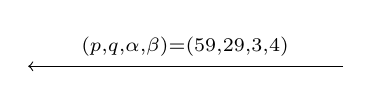
\begin{tikzpicture}
        \draw[->] (4,-0.75)--(0,-0.75);
        \node at (2,-0.5){$_{(p,q,\alpha,\beta)=(59,29,3,4)}$};
    \end{tikzpicture}
    \begin{tabular}{l@{\hskip 11cm}l}
        &signature generation:\\
        &compute hash of message $h(x)=26$;\\
        &choose ephemeral key $k_E=10$;\\
        &$r=(3^{10}\mymod59)\equiv20\mymod29$;\\
        &$s=(26+7\cdot20)\cdot3\equiv5\mymod29$;
    \end{tabular}
    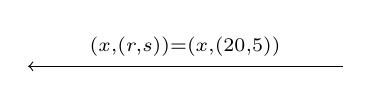
\begin{tikzpicture}
        \draw[->] (4,-0.75)--(0,-0.75);
        \node at (2,-0.5){$_{(x,(r,s))=(x,(20,5))}$};
    \end{tikzpicture}\\
    \begin{tabular}{l@{\hskip 11cm}l}
        signature verification:&\\
        $w=5^{-1}\equiv6\mymod29$&\\
        $u_1=6\cdot26\equiv11\mymod29$&\\
        $u_2=6\cdot20\equiv4\mymod29$&\\
        $v=(3^{11}\cdot4^4\mymod59)\mymod29=20$&\\
        $v\equiv r\mymod29\Longrightarrow\text{valid signature}$&
    \end{tabular}
\end{framed}
\end{center}

\subsubsection{Computational aspects}
The most demanding part is the key-generation phase. However, this phase only has to be executed once at set-up time.

\subsubsection*{Key Generation}
The challenge in the key-generation phase is to find a cyclic group $\mathbb{Z}_p^*$ with a bit length of 1024, and which has a prime subgroup in the range of $2^{160}$. This condition is fulfilled if $p-1$ has a prime factor \textit{q} of 160 bits. The general approach to generating such parameters is to first find the 160-bit prime \textit{q} and then to construct the larger prime \textit{p} from it.

\subsubsection*{Signing}
During signing we compute the parameters \textit{r} and \textit{s}. Computing \textit{r} involves first evaluation $\alpha^{k_E}\mymod p$ using the square-and-multiply algorithm. Since $k_E$ has only 160 bits, about 240 squarings and multiplications are required on average, even though the arithmetic is done with 1024-bit numbers. The result, which has also a length of 1024 bits, is then reduced to 160 bits by the operation$\pmod q$. Computing \textit{s} involves only 160-bit numbers. The most costly step is the inversion of $k_E$.

\subsubsection*{Verification}
Computing the auxiliary parameters \textit{w}, $u_1$ and $u_2$ only involves 160-bit operands, which makes verification relatively fast.

\newpage
\subsection{Past Exams Exercises (DSA)}
\subsubsection{2020-07-03 ex. 3}
Alice generates a secret key $\text{SK}_{\text{A}}=d=4$ and wants to generate a DS. Given that the prime numbers are $p=11$ and $q=5$, what is the public key?

\subsubsection*{Solution}
As we've previously mentioned, the public key in the DSA is defined as $k_{pub}=(p,q,\alpha,\beta)$. Since we already know $p$ and $q$, we must find $\alpha$ such that $\text{ord}(\alpha)=q$. Remember that:
\begin{itemize}
    \item we're working in $\mathbb{Z}_p^*=\mathbb{Z}_{11}^*=\{1,2,...,10\}$;
    \item the subgroup generated by $\alpha$ has cardinality equal to $q=5$;
\end{itemize}
In order to find $\alpha$ we must find the element of $\mathbb{Z}_{11}^*$ that generates the subgroup. So, we must look for that element $\alpha\in \mathbb{Z}_{11}^*$ such that $\alpha^5=\idElement$ and $\alpha\not=\idElement$. Let's test all elements starting from 2:
\begin{align*}
    &2^5=32\equiv10\mymod11\\
    &3^5=3^3\cdot3^2\equiv5\cdot9\equiv1\mymod11\\
    &...
\end{align*}
So, 3 is a generator of the subgroup. We can indeed verify that:
\begin{align*}
    &3^1=3\\
    &3^2\equiv9\mymod11\\
    &3^3\equiv5\mymod11\\
    &3^4\equiv4\mymod11\\
    &3^5\equiv1\mymod11
\end{align*}
So the subgroup is $H=\{1,3,4,5,9\}$.\\\\
We can now compute $\beta$ as:
$$\beta\equiv\alpha^d\mymod p\longrightarrow\beta=3^4\equiv 4\mymod 11$$
In the end, the public key is:
$$k_{pub}=(11,5,3,4)$$

\newpage
\subsubsection{2021-09-14 ex. 4}
DSA algorithm. Given $p=11$, $q=5$ and $d=4$,  what is the public key?
\begin{itemize}
    \item[a)] (11,5,9,5);
    \item[b)] (11,5,3,5);
    \item[c)] (11,5,7,3);
    \item[d)] (11,5,2,4);
    \item[e)] (11,5,4,2);
\end{itemize}

\subsubsection*{Solution}
The fastest way to solve the exercise is to test the given values of $\alpha$ and $\beta$ to see if both the following conditions are satisfied:
\begin{itemize}
    \item $\alpha^5\equiv1\mymod11$;
    \item $\beta\equiv\alpha^d\mymod11$;
\end{itemize}
Let's test the conditions:
\begin{itemize}
    \item[a)] $9^5=9^2\cdot9^2\cdot9\equiv4\cdot4\cdot9\equiv5\cdot9=45\equiv1\mymod11$ \textcolor{Green}{\checkmark}\\
    $9^4=9^2\cdot9^2\equiv4\cdot4\equiv5\mymod11$ \textcolor{Green}{\checkmark}
    \item[b)] $3^5=3^3\cdot3^2\equiv5\cdot9\equiv1\mymod11$ \checkmark\\
    $3^4=3^3\cdot3\equiv5\cdot3\equiv4\not\equiv5\mymod11$
    \item[c)] $7^5=7^2\cdot7^2\cdot7\equiv5\cdot5\cdot7\equiv3\cdot7\equiv10\not\equiv1\mymod11$
    \item[d)] $2^5=32\equiv10\not\equiv1\mymod11$
    \item[e)] $4^5=4^2\cdot4^2\cdot4\equiv5\cdot5\cdot4\equiv3\cdot4\equiv1\not\equiv2\mymod11$
\end{itemize}
So, the right answer is (a).

\newpage
\subsection{Exercises from slides (DSA)}
\subsubsection{Exercise 10.4.6}
Set $p=59$, $q=29$, $\alpha=3$, $d=7$, $\beta=\alpha^d\mymod59$. Assuming that $SHA(x)=26$ compute the DSA $sig(r,s)$.

\subsubsection*{Solution}
Let's compute $r$ first. Let's choose a random value for the ephemeral key: $0<k_E=21<q$
\begin{align*}
    r&\equiv(\alpha^{k_E}\mymod p)\mymod q=\\
    &=(3^{21}\mymod59)\mymod29=\\
    &=\left[(3^4)^5\cdot3\mymod59\right]\mymod29=\\
    &=\left(81^5\cdot3\mymod59\right)\mymod29\equiv\\
    &\equiv\left(22^5\cdot3\mymod59\right)\mymod29=\\
    &=\left(22^2\cdot22^2\cdot22\cdot3\mymod59\right)\mymod29\equiv\\
    &\equiv(12\cdot12\cdot22\cdot3\mymod59)\mymod29=\\
    &=(144\cdot66\mymod59)\mymod29\equiv\\
    &\equiv(26\cdot7\mymod59)\mymod29\equiv\\
    &\equiv(5\mymod59)\mymod29\equiv\\
    &\equiv5\mymod29
\end{align*}
Now, let's compute $s$:
\begin{align*}
    s&\equiv(SHA(x)+d\cdot r)k_E^{-1}\mymod q=\\
    &=(26+7\cdot5)21^{-1}\mymod29=\\
    &=61\cdot21^{-1}\mymod29\equiv\\
    &\equiv3\cdot18\mymod29=\\
    &=25\mymod29
\end{align*}
Note that the inverse $21^{-1}\mymod29$ can be calculated with the EEA as explained in the dedicated chapter.\\\\
In the end, the signature is:
$$sig=(5,25)$$
For completeness, let's perform the verification of the signature:
\begin{itemize}
    \item Computation of the hash of the message (already provided by the text): $SHA(x)=26$;
    \item Auxiliary values computation:
    \begin{alignat*}{3}
        w&\equiv s^{-1}\mymod q&&\longrightarrow w&&=25^{-1}\equiv7\mymod29\\
        u_1&\equiv w\cdot SHA(x)\mymod q&&\longrightarrow u_1&&=7\cdot26=182\equiv8\mymod29\\
        u_2&\equiv w\cdot r\mymod q&&\longrightarrow u_2&&=7\cdot5=35\equiv6\mymod29
    \end{alignat*}
    \item Final computation + verification:
    \begin{align*}
        v&\equiv(\alpha^{u_1}\cdot\beta^{u_2}\mymod p)\mymod q\equiv\\
        &\equiv(3^8\cdot3^{42}\mymod 59)\mymod29=(3^{50}\mymod59)\mymod29\equiv\\
        &\equiv (5\mymod59)\mymod29\equiv5\mymod29\equiv r\text{ \textcolor{Green}\checkmark}
    \end{align*}
\end{itemize}

\newpage
\section{Elliptic Curve Cryptography (ECC)}
ECC provides the same level of security as RSA or Discrete Logarithm (DL) systems with considerably shorter operands (approximately 160-256 bit vs. 1024-3072 bit). ECC is based on the generalized discrete logarithm problem. ECC has performance advantages (fewer computations) and bandwidth advantages (shorter signatures and keys) over RSA and DL schemes. However, RSA operations which involve short public keys are still much faster than ECC operations.

\subsection{The Generalized Discrete Logarithm Problem (GDLP)}
\begin{framed}
    \hfill\break\textbf{Definition} Discrete Logarithm Problem (DLP) in $\mathbb{Z}_p^*$\\
    \textit{Given the finite cyclic group $\mathbb{Z}_p^*$ of order $p-1$ and a generator $\alpha\in\mathbb{Z}_p^*$ and another element $\beta\in\mathbb{Z}_p^*$, the DLP is the problem of determining the integer $1\le x\le p-1$ such that:}
    $$\alpha^x\equiv \beta\mymod p$$
\end{framed}
\begin{framed}
    \hfill\break\textbf{Definition} Generalized Discrete Logarithm Problem\\
    \textit{Given a finite cyclic group $G$ with the group operation $\circ$ and cardinality $n$. We consider a generator $\alpha\in G$ and another element $\beta\in G$. The GDLP is finding the integer $x$, where $1\le x\le n$, such that:}
    $$\beta=\underbrace{\alpha\circ\alpha\circ...\circ\alpha}_{x\text{ times}}=\alpha^x$$
\end{framed}

\subsection{Definition of Elliptic Curves}
Since ECC is based on the GDLP, we need to find a cyclic group on which we can build our cryptosystem. Of course, the mere existence of a cyclic group is not sufficient, as the DL problem in this group must also be computationally hard.\\\\
An Elliptic Curve is a special type of polynomial equation. For cryptographic use, we need to consider the curve not over the real numbers but over a finite field. The most popular choice is Galois fields $GF(p)$, where all arithmetic is performed modulo a prime \textit{p}.
\begin{framed}
    \hfill\break\textbf{Definition} Elliptic Curve\\
    \textit{The elliptic curve over} $\mathbb{Z}_p$, $p>3$, \textit{is the set of all pairs $(x,y)\in\mathbb{Z}_p$ which fulfill}
    $$y^2\equiv x^3+a\cdot x+b\mymod p$$
    \textit{together with an imaginary} \textbf{point of infinity \textit{O}}\textit{, where}
    $$a,b\in\mathbb{Z}_p$$
    \textit{and the condition $4\cdot a^3+27\cdot b^2\not=0\mymod p$.}
\end{framed}
The definition requires that the curve is nonsingular, i.e., the plot has no self-intersections or vertices, which is achieved if the discriminant of the curve $-16(4a^3+27b^2)$ is nonzero. For cryptographic use we are interested in studying the curve over a prime field as in the definition. However, if we plot such an elliptic curve over $\mathbb{Z}_p$, we do not get anything remotely resembling a curve. However, nothing prevents us from taking an elliptic curve equation and plotting it over the set of real numbers.

\newpage
\hfill\break
The first step for finding a group is identifying a set of elements for the group:
\begin{itemize}
    \item the group elements are basically the points that fulfill the Elliptic Curve equation:$$y^2\equiv x^3+a\cdot x+b\mymod p$$
\end{itemize}
Now we must define a new set of group operations with such elements...

\subsection{Group Operations on Elliptic Curves}
Let's denote the group operation with the addition symbol \doublequotes{+}. \doublequotes{Addition} means that given two points and their coordinates, say $P_1=(x_1,y_1)$ and $P_2=(x_2,y_2)$, we have to compute the coordinates of a third point $Q$ such that:
$$P_1+P_2=Q$$
$$(x_1,y_1)+(x_2,y_2)=(x_3,y_3)$$
Keep in mind that the \doublequotes{+} symbol doesn't refer to the classic addition operation we're used to, as we're defining a new kind of operation (the group operation).

\subsubsection{Point Addition and Point Doubling}
There is a nice geometric interpretation of the addition operation if we consider a curve defined over the real numbers. For this interpretation, we have to distinguish two cases: the addition of two distinct points (named \doublequotes{point addition}) and the addition of one point to itself (named \doublequotes{point doubling}):
\begin{itemize}
    \item \textbf{Point Addition} This is the case where we compute $Q=P_1+P_2$ and $P_1\not=P_2$. The construction works as follows: draw a line through $P_1$ and $P_2$ and obtain a third point of intersection between the elliptic curve and the line. Mirror this third intersection point along the \textit{x}-axis. This mirrored point is, by definition, the point $Q$;
    \item \textbf{Point Doubling} This is the case where we compute $P_1+P_2$ but $P_1=P_2$. Hence, we can write $Q=P+P=2P$. We need a slightly different construction here. We draw the tangent line through $P$ and obtain a second point of intersection along the \textit{x}-axis. This mirrored point is the result $Q$ of doubling;
\end{itemize}
\begin{figure}[H]
    \centering
    \includegraphics[scale=0.75]{EC/1.png}
\end{figure}
If points on the elliptic curve are \textit{added} in this very way, the set of points also fulfill most conditions necessary for a group, that is, closure, associativity, existence of an identity element and existence of an inverse. Of course, in a cryptosystem we cannot perform geometric constructions. However, by applying simple coordinate geometry, we can express both of the geometric constructions from above through analytic expressions. These formulae only involve the four basic algebraic operations.

\newpage
\hfill\break
These operations can be performed in any field, not only over the field of the real numbers. In particular, we can take the curve equation from above, but we now consider it over Galois fields $GF(p)$ rather than over the real numbers. This yields the following analytical expressions for the group operation.
\begin{framed}
    \hfill\break\textbf{Elliptic Curve Point Addition and Point Doubling}
    \begin{align*}
        &x_3=s^2-x_1-x_2\mymod p\\
        &y_3=s(x_1-x_3)-y_1\mymod p
    \end{align*}
    where
    \begin{equation*}
        s=\begin{cases}
            \dfrac{y_2-y_1}{x_2-x_1}\mymod p; \text{ if $P_1\not=P_2$ (point addition)}\\\\
            \dfrac{3x_1^2+a}{2y_1}\mymod p; \text{ if $P_1=P_2$ (point doubling)}
        \end{cases}
    \end{equation*}
\end{framed}
Note that the parameter $s$ is the slope of the line through $P_1$ and $P_2$ in the case of point addition, or the slope of the tangent through $P$ in the case of point doubling.

\subsubsection{Identity element}
Even though we defined the operations above, we're not done yet. One thing that is still missing is an identity (or neutral) element \textit{\textbf{O}} such that:
$$P+\text{\textbf{\textit{O}}}=P$$
for all points $P$ on the elliptic curve. It turns out that there isn't any point $(x,y)$ that fulfills the condition. Instead we define an \textit{abstract point at infinity} as the neutral element \textbf{\textit{O}}. This point at infinity can be visualized as a point that is located either towards $+\infty$ or towards $-\infty$ along the \textit{y}-axis.

\subsubsection{Inverse element}
We can now also define the inverse $-P$ of any group element $P$ as:
$$P+(-P)=\text{\textbf{\textit{O}}}$$
The question is how do we find $-P$? If we apply the tangent-and-chord method from above, it turns out that the inverse of the point $P=(x_p,y_p)$ is the point $-P=(x_p,-y_p)$, i.e., the point that is reflected along the \textit{x}-axis. Note that finding the inverse of a point $P=(x_p,y_p)$ is now trivial. We simply take the negative of its $y$ coordinate. In the case of elliptic curves over a Galois field $GF(p)$, this is easily achieved since $-y_p\equiv p-y_p\mymod p$, hence:
$$-P=(x_p,p-y_p)$$

\newpage
\hfill\break
Now that we have defined all group properties for elliptic curves, we can look at an example:\\

\textit{Example)} We consider a curve over the field $\mathbb{Z}_{17}$:
$$E:y^2\equiv x^3+2x+2\mymod 17$$

We want to double the point $P=(5,1)$.
\begin{align*}
    2P&=P+P=(5,1)+(5,1)=(x_3,y_3)\\
    s&=\dfrac{3x_1^2+a}{2y_1}=(2\cdot1)^{-1}(3\cdot5^2+2)=2^{-1}\cdot77\equiv9\cdot9\equiv13\mymod 17\\
    x_3&=s^2-x_1-x_2=13^2-5-5=159\equiv6\mymod17\\
    y_3&=s(x_1-x_3)-y_1=13(5-6)-1=-14\equiv3\mymod17\\
    2P&=(5,1)+(5,1)=(6,3)
\end{align*}

For illustrative purposes we check whether the result $2P=(6,3)$ is actually a point on the

curve by inserting the coordinates into the curve equation:
\begin{align*}
    y^2&\equiv x^3+2x+2\mymod17\\
    3^2&\equiv6^3+2\cdot6+2\mymod17\\
    9&\equiv230\equiv9\mymod 17 \text{ \checkmark}
\end{align*}

\subsection{Building a Discrete Logarithm Problem with Elliptic Curves}
What we have done so far is to establish the group operations (point addition and doubling), we have provided an identity element and we have shown a way of finding the inverse for any point on the curve. Thus, we now have all necessary requirements in place to motivate the following theorem:
\begin{framed}
    \hfill\break\textbf{Theorem} \textit{The points on an elliptic curve together with \textbf{O} have cyclic subgroups. Under certain conditions all points on an elliptic curve form a cyclic group.}
\end{framed}
This theorem is extremely useful because we already have a good understanding of the properties of cyclic groups. In particular, we know that by definition a generator must exist such that its powers generate the entire group. Moreover, we know quite well how to build cryptosystems from cyclic groups. So, we can now have a look at an example for the cyclic group of an elliptic curve.\\\\
\textit{Example)} We want to find all points on the curve:$$E:y^2\equiv x^3+2x+2\mymod17.$$
It happens that all points on the curve form a cyclic group and that the order is $\#E=19$.\\
For this specific curve the group order is a prime and so every element (point) is a generator. For simplicity we choose to compute all the curve points starting from the same point of the previous example, that is the element $P=(5,1)$. So, we compute all \doublequotes{powers} of $P$. More precisely, since the group operation is addition, we compute $P,2P,...,(\#E)P$.

\newpage
\hfill\break
Here's what we obtain:
\begin{itemize}
    \item $2P=(5,1)+(5,1)=(6,3)$;
    \item $3P=2P+P=(6,3)+(5,1)=(10,6)$
    \begin{itemize}
        \item[] $s=\dfrac{y_2-y_1}{x_2-x_1}=\dfrac{3-1}{6-5}=2\mymod 17$
        \item[] $x_3=s^2-x_1-x_2=4-5-6=-7\equiv10\mymod17$
        \item[] $y_3=s(x_1-x_3)-y_1=2(5-10)-1=-11\equiv6\mymod17$
    \end{itemize}
    \item $4P=(3,1)$
    \begin{itemize}
        \item Calculated with point addition as $3P+P=(10,6)+(5,1)$:
        \begin{alignat*}{3}
            s&=\dfrac{y_2-y_1}{x_2-x_1}&&=\dfrac{6-1}{10-5}&&\equiv1\mymod 17\\
            x_3&=s^2-x_1-x_2&&=1-5-10=-14&&\equiv3\mymod17\\
            y_3&=s(x_1-x_3)-y_1&&=(5-3)-1&&\equiv1\mymod17
        \end{alignat*}
        \item Calculated with point doubling as $2P+2P=(6,3)+(6,3)$:
        \begin{alignat*}{3}
            s&=\dfrac{3x^2+a}{2y}&&=\dfrac{108+2}{6}=3^{-1}\cdot55\equiv6\cdot4&&\equiv7\mymod 17\\
            x_3&=s^2-2x&&=49-12=37&&\equiv3\mymod17\\
            y_3&=s(x-x_3)-y&&=7(6-3)-3=18&&\equiv1\mymod17
        \end{alignat*}
    \end{itemize}
    As we can see, by using point doubling we can focus on the coordinates of a single point $(x,y)$ but the modular arithmetic could be a bit more complex (it obviously depends from case to case);
    \item \begin{alignat*}{2}
        5P&=(9,16)\hspace{3cm}&&12P=(0,11)\\
        6P&=(16,13)&&13P=(16,4)\\
        7P&=(0,6)&&14P=(9,1)\\
        8P&=(13,7)&&15P=(3,16)\\
        9P&=(7,6)&&16P=(10,11)\\
        10P&=(7,11)&&17P=(6,14)\\
        11P&=(13,10)&&18P=(5,16)
    \end{alignat*}
    \item $19P=\text{\textbf{\textit{O}}}$
    \begin{itemize}
        \item Calculated with point addition as $18P + P = (5, 16) + (5, 1)$:
        $$s=\dfrac{16-1}{5-5}=\ ?$$
        As we can see, we can't calculate $s$. That's because $18P$ and $P$ are the inverse of each other. This is easy to verify. Since we've already checked that the two $x$ coordinates are identical, we just have to check that the two $y$ coordinates are each other's additive inverse modulo 17. As we've already seen, the inverse of a point $P=(x_p,y_p)$ is $-P=(x_p,-y_p)$. Let's compute the inverse of $18P$:
        $$-18P=(5,-16)\equiv(5,1)\mymod17=P$$
        So, $18P$ and $P$ are indeed the inverse of each other. So:
        $$19P=18P+P=\text{\textbf{\textit{O}}}$$
    \end{itemize}
\end{itemize}
\textit{End of the Example.}

\newpage
\hfill\break
To set up a DL cryptosystem it is important to know the order of the group. Even though knowing the exact number of points on a curve is an elaborate task, we know the approximate number due to \textit{Hasse's theorem}:
\begin{framed}
    \hfill\break\textbf{Theorem} Hasse's theorem\\
    \textit{Given an elliptic curve E modulo p, the number of points on the curve is denoted by \#E and is bounded \nolinebreak by:}
    $$p+1-2\sqrt{p}\le\#E\le p+1+2\sqrt{p}$$
\end{framed}
Hasse's theorem, which is also known as \textit{Hasse's bound}, states that the number of points is roughly in the range of the prime $p$. This has major practical implications. For instance, if we need an elliptic curve with $2^{160}$ elements, we have to use a prime of length of about 160 bit.\\\\
Let's now turn our attention to the details of setting up the discrete logarithm problem. For this, we can strictly proceed as following:
\begin{framed}
    \hfill\break\textbf{Definition} Elliptic Curved Discrete Logarithm Problem (ECDLP)\\
    \textit{Given an elliptic curve E, we consider a generator P and another element T. The DL problem is finding the integer d, where $1\le d\le\#E$, such that:}
    $$\underbrace{P+P+\cdots+P}_{d\text{ times}}=dP=T$$
\end{framed}
In cryptosystems, $d$ is the private key which is an integer, while the public key $T$ is a point on the curve with coordinates $T=(x_{_T},y_{_T})$. In contrast, in the case of the DL problem in $\mathbb{Z}_p^*$, both keys were integers. The operation shown in the theorem above is called \textit{\textbf{point multiplication}}, since we can formally write $T=dP$. So, $dP$ is merely a convenient notation for the repeated application of the group operation.\\\\
Point multiplication is analog to exponentiation in multiplicative groups. In order to do it efficiently, we can directly adopt the square-and-multiply algorithm. The only difference is that squaring becomes (point) doubling and multiplication becomes (point) addition of $P$. We can call this \textbf{\textit{Double-and-Add algorithm}}.\\\\
\textit{Example)} We consider the scalar multiplication $26P$, which has the following binary representation:
$$26P=(11010_2)P=(d_4d_3d_2d_1d_0)_2P$$
The algorithm scans the scalar bits starting on the left with $d_4$ and ending with the rightmost bit $d_0$. The initialization value for the algorithm is \textbf{\textit{O}}:
\begin{enumerate}
    \item[0)] $d_4=1\rightarrow res_0=2\text{\textbf{\textit{O}}}+P=P$
    \item[1)] $d_3=1\rightarrow res_1=2res_0+P=2P+P=3P$
    \item[2)] $d_2=0\rightarrow res_2=2res_1=6P$
    \item[3)] $d_1=1\rightarrow res_3=2res_2+P=12P+P=13P$
    \item[4)] $d_0=0\rightarrow res_4=2res_3=26P$
\end{enumerate}
There's a nice geometric interpretation for the ECDLP: given a starting point $P$, we compute $2P,3P,...,dP=T$, effectively hopping back and forth on the elliptic curve. We then publish the starting point $P$ (a public parameter) and the final point $T$ (the public key). In order to break the cryptosystem, an attacker has to figure out how often we \doublequotes{jumped} on the elliptic curve. The number of hops is the secret $d$, the private key.

\newpage
\subsection{Elliptic Curve Protocols}
\subsubsection{Diffie-Hellman Key Exchange with Elliptic Curves (ECDH)}
We can now realize a key exchange using elliptic curves. This is referred to as Elliptic Curve Diffie-Hellman key exchange, or ECDH. First, we have to agree on domain parameters, that is, a suitable elliptic curve over which we can work and a generator on this curve.
\begin{framed}
    \hfill\break\textbf{ECDH Domain Parameters}
    \begin{enumerate}
        \item Choose a prime $p$ and the elliptic curve
        $$E:y^2\equiv x^3+a\cdot x+b\mymod p$$
        \item Choose a generator $P=(x_{_P},y_{_P})$
    \end{enumerate}
    The prime $p$, the curve given by its coefficients $a$, $b$, and the generator $P$ are the domain parameters.
\end{framed}
Note that, in practice, finding a suitable elliptic curve is a relatively difficult task. The curves have to show certain properties in order to be secure. The actual key exchange is done the same way it was done for the conventional Diffie-Hellman protocol.
\begin{framed}
    \hfill\break\textbf{Elliptic Curve Diffie-Hellman Key Exchange}
    \begin{center}
        \begin{tabular}{c@{\hskip 3cm}c}
            \textbf{Alice}&\textbf{Bob}\\
            choose $k_{prA}=a\in\{2,3,...,\#E-1\}$&choose $k_{prB}=b\in\{2,3,...,\#E-1\}$\\
            compute $k_{pubA}=aP=A=(x_A,y_A)$&compute $k_{pubB}=bP=B=(x_B,y_B)$
        \end{tabular}
        \begin{tikzpicture}
            \draw[->] (0,0)--(4,0);
            \node at (2,0.25){$_A$};
            \draw[->] (4,-0.75)--(0,-0.75);
            \node at (2,-0.5){$_B$};
        \end{tikzpicture}
    \end{center}
    \hspace{2.5cm}compute $aB=T_{AB}$\hspace{5.875cm}compute $bA=T_{AB}$
\end{framed}\hfill\break
Since point addition is associative, both parties compute the same result, namely the point $T_{AB}=abP$.\\

As we can see in the protocol, Alice and Bob choose the private keys $a$ and $b$, respectively, which are two large integers. With the private keys they both generate their respective public keys $A$ and $B$, which are points on the curve. The public keys are computed by point multiplication. The two parties exchange these public parameters with each other. The joint secret $T_{AB}$ is then computed by both Alice and Bob by performing a second point multiplication involving the public key they received and their own secret parameter. The joint secret $T_{AB}$ can be used to derive a session key, e.g., as input for the AES algorithm. Note that the two coordinates $(x_{_{AB}},y_{_{AB}})$ are not independent of each other: given $x_{_{AB}}$, the other coordinate can be computed by simply inserting the $x$ value in the elliptic curve equation. Thus, only one of the two coordinates should be used for the derivation of a session key.\\\\
In practice, often the $x$-coordinate is hashed and then used as a symmetric key. Typically, not all bits are needed. For instance, in a 160-bit ECC scheme, hashing the $x$-coordinate with SHA-1 results in a 160-bit output of which only 128 bit would be used as an AES key.

\newpage
\subsubsection{Elliptic Curve Digital Signature Algorithm (ECDSA)}
The steps in the ECDSA standard are conceptually closely related to the DSA scheme. However, its DLP is constructed in the group of an elliptic curve. Thus, the arithmetic to be performed for actually computing the signature is entirely different from that used for DSA. The ECDSA standard is defined for elliptic curves over prime fields $\mathbb{Z}_p$ and Galois Fields $GF(2^m)$. The former  is often preferred in practice, and we will only introduce this one in what follows.

\subsubsection*{Key Generation}
The keys for the ECDSA are computed as follows:
\begin{framed}
    \hfill\break\textbf{Key Generation for ECDSA}
    \begin{enumerate}
        \item Use an elliptic curve $E$ with
        \begin{itemize}
            \item modulus $p$;
            \item coefficients $a$ and $b$;
            \item a point $A$ which generates a cyclic group of prime order $q$;
        \end{itemize}
        \item Choose a random integer $d$ with $0<d<q$;
        \item Compute $B=dA$.
    \end{enumerate}
    The keys are now:
    $$k_{pub}=(p,a,b,q,A,B)$$
    $$k_{pr}=(d)$$
\end{framed}
Note that we have set up a DLP where the integer $d$ is the private key and the result of the scalar multiplication, point $B$, is the public key. Similar to DSA, the cyclic group has an order $q$ which should have a size of at least 160 bit or more for higher security levels.

\subsubsection*{Signature and Verification}
Like DSA, an ECDSA signature consists of a pair of integers $(r,s)$. Each value has the same bit length as $q$, which makes for fairly compact signatures. Using the public and private key, the signature for a message $x$ is computed as follows:
\begin{framed}
    \hfill\break\textbf{ECDSA Signature Generation}
    \begin{enumerate}
        \item Choose an integer as random ephemeral key $k_E$ with $0<k_E<q$;
        \item Compute $R=k_EA$;
        \item Let $r=x_R$;
        \item Compute $s\equiv (h(x)+d\cdot r)k_E^{-1}\mymod q$;
        \item The signature of the message $x$ with the secret key $d$ is:
        $$sig_d(x,k_E)=(r,s)$$
    \end{enumerate}
\end{framed}
In step 3 the $x$-coordinate of the point $R$ is assigned to the variable $r$. The message $x$ has to be hashed using the function $h$ in order to compute $s$. The hash function output length must be at least as long as $q$.

\newpage
\hfill\break
The signature verification process is as follows:
\begin{framed}
    \hfill\break\textbf{ECDSA Signature Verification}
    \begin{enumerate}
        \item Compute auxiliary value $w\equiv s^{-1}\mymod q$;
        \item Compute auxiliary value $u_1\equiv w\cdot h(x)\mymod q$;
        \item Compute auxiliary value $u_2\equiv w\cdot r\mymod q$;
        \item Compute $P=u_1A+u_2B$;
        \item The verification $ver_{k_{pub}}(x,(r,s))$ follows from:
        \begin{equation*}
            x_P\begin{cases}
                \equiv r\mymod q\Longrightarrow\text{valid signature}\\
                \not\equiv r\mymod q\Longrightarrow\text{invalid signature}
            \end{cases}
        \end{equation*}
    \end{enumerate}
\end{framed}
\hfill\break
\textit{Example)} Bob wants to send a message to Alice that is to be signed with the ECDSA. The signature and verification process is as follows:
\begin{center}
\begin{framed}
    \begin{tabular}{c@{\hskip 10cm}c}
        \textbf{Alice}&\textbf{Bob}
    \end{tabular}
    \begin{tabular}{l@{\hskip 11cm}l}
        &key generation:\\
        &choose $E$ with $p=17$, $a=2$, $b=2$,\\
        &and $A=(5,1)$ with $q=19$;\\
        &choose $d=7$;\\
        &compute $B=dA=7\cdot(5,1)=(0,6)$;
    \end{tabular}
    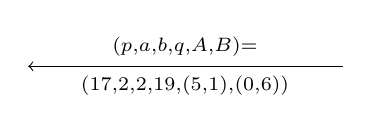
\begin{tikzpicture}
        \draw[->] (4,-0.75)--(0,-0.75);
        \node at (2,-0.5){$_{(p,a,b,q,A,B)=}$};
        \node at (2,-1){$_{(17,2,2,19,(5,1),(0,6))}$};
    \end{tikzpicture}
    \begin{tabular}{l@{\hskip 11cm}l}
        &signature generation:\\
        &compute hash of message $h(x)=26$;\\
        &choose ephemeral key $k_E=10$;\\
        &$R=10\cdot(5,1)=(7,11)$;\\
        &$r=x_R=7$;\\
        &$s=(26+7\cdot7)\cdot2\equiv17\mymod19$;
    \end{tabular}
    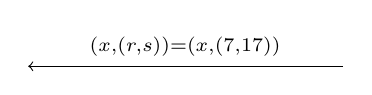
\begin{tikzpicture}
        \draw[->] (4,-0.75)--(0,-0.75);
        \node at (2,-0.5){$_{(x,(r,s))=(x,(7,17))}$};
    \end{tikzpicture}\\
    \begin{tabular}{l@{\hskip 11cm}l}
        signature verification:&\\
        $w=17^{-1}\equiv9\mymod19$&\\
        $u_1=9\cdot26\equiv6\mymod19$&\\
        $u_2=9\cdot7\equiv6\mymod19$&\\
        $P=6\cdot(5,1)+6\cdot(0,6)=(7,11)$&\\
        $x_P\equiv r\mymod19\Longrightarrow\text{valid signature}$&
    \end{tabular}
\end{framed}
\end{center}
Note that we chose the elliptic curve
$$E:y^2\equiv x^3+2x+2\mymod17$$
which we already used in previous examples, because all of its points form a cyclic group of order 19, i.e., a prime, there are no subgroups and hence in this case $q=\#E=19$.

\newpage
\subsection{Past Exams Exercises (Elliptic Curves)}
\subsubsection{2022-06-27/2021-07-02 ex. 1 v.1}
Let $E:y^2\equiv x^3+2x+2\mymod 17$, $P=(5,1)$ and $Q=(6,3)$, such that $P+Q+R=\text{\textbf{\textit{O}}}$. Compute $R$.
\subsubsection*{Solution}
It's straightforward that:
$$R=-P+(-Q)$$
Where $-P$ and $-Q$ are the inverses of $P$ and $Q$:
$$-P=(5, -1)\equiv(5,16)\mymod17$$
$$-Q=(6,-3)\equiv(6,14)\mymod17$$
Let's perform the point addition
$$R=(5,16)+(6,14)=(x_R,y_R)$$
by computing all the necessary parameters:
\begin{alignat*}{4}
    s&=\dfrac{y_2-y_1}{x_2-x_1}&&=\dfrac{16-14}{5-6}=1^{-1}\cdot (-2)&&\equiv 1^{-1}\cdot 15&&\equiv15\mymod17\\
    x_R&=s^2-x_2-x_1&&=15^2-5-6&&=214&&\equiv10\mymod17\\
    y_R&=s(x_1-x_R)-y_1&&=15(6-10)-14&&=-74&&\equiv11\mymod17
\end{alignat*}
So, we obtain:
$$R=(10,11)$$

\subsubsection{2021-07-02 ex. 1 v.2}
Let $E:y^2\equiv x^3+2x+2\mymod 17$, $P=(6,3)$ and $Q=(10,6)$, such that $P+Q+R=\text{\textbf{\textit{O}}}$. Compute $R$.
\subsubsection*{Solution}
As in the previous exercise:
\begin{alignat*}{3}
    -P&=(6,-3)&&\equiv(6,14)&&\mymod17\\
    -Q&=(10,-6)&&\equiv(10,11)&&\mymod17
\end{alignat*}
We perform the point addition
$$R=(6,14)+(10,11)=(x_R,y_R)$$
by computing all the necessary parameters:
\begin{alignat*}{4}
    s&=\dfrac{y_2-y_1}{x_2-x_1}&&=\dfrac{14-11}{6-10}=4^{-1}\cdot (-3)&&\equiv 13\cdot 14=182&&\equiv12\mymod17\\
    x_R&=s^2-x_2-x_1&&=12^2-6-10&&=128&&\equiv9\mymod17\\
    y_R&=s(x_1-x_R)-y_1&&=12(10-9)-11&&=1&&\equiv1\mymod17
\end{alignat*}
So, we obtain:
$$R=(9,1)$$

\newpage
\subsubsection{FacsimileCryptography 2020 ex.2/Random.pdf}
Let $E:y^2\equiv x^3+7$ be the elliptic curve defined on $\mathbb{Z}_{11}$.
\begin{itemize}
    \item[(a)] Check that $P=(2,2)$ and $Q=(7,3)$ are in $E$;
    \item[(b)] Compute the addition $P+Q$ on the elliptic curve $E$;
    \item[(c)] Check that your answer to (b) is a point of $E$;
\end{itemize}

\subsubsection*{Solution}
\begin{itemize}
    \item[(a)] To check if a point $P$ belongs to the curve, we simply check that the curve equation is still satisfied after replacing $x,y$ with $x_P,y_P$.
    \begin{itemize}
        \item P belongs to the curve
        $$4\stackrel{\text{?}}{\equiv}15\ \longrightarrow\ 4\equiv4\mymod11\text{ \checkmark}$$
        \item Q belongs to the curve
        $$9\stackrel{\text{?}}{\equiv}7\cdot7^2+7=7(7^2+1)\equiv7\cdot6=42\ \longrightarrow\ 9\equiv9\mymod11\text{ \checkmark}$$
    \end{itemize}
    \item[(b)] Let's compute the result of the point addition $R=(2,2)+(7,3)=(x_R,y_R)$.
    \begin{alignat*}{4}
        s&=\dfrac{y_2-y_1}{x_2-x_1}&&=\dfrac{2-3}{2-7}&&=5^{-1}&&\equiv9\mymod11\\
        x_R&=s^2-x_2-x_1&&=81-2-7&&=72&&\equiv6\mymod11\\
        y_R&=s(x_1-x_R)-y_1&&=9(7-6)-3&&=6&&\equiv6\mymod11
    \end{alignat*}
    So, we obtain:
    $$R=P+Q=(6,6)$$
    \item[(c)] R belongs to the curve
    $$36\stackrel{\text{?}}{\equiv}6\cdot6^2+7\equiv6\cdot3+7=25\ \longrightarrow\ 3\equiv3\mymod11\text{ \checkmark}$$
\end{itemize}

\newpage
\subsection{Exercises from slides (Elliptic Curves)}
\subsubsection{Exercise 11.3.2}
Let $G=(5,1)$ be a point of $E:\ y^2\equiv x^3+2x+2\mymod17$. Find:
\begin{itemize}
    \item $P\in E$ such that $18P=(0,6)$;
    \item $Q\in E$ such that $3Q=(3,16)$;
\end{itemize}
Here's the table of all multiples of $G$:
\begin{alignat*}{2}
    G&=(5,1)\hspace{4cm}&&10G=(7,11)\\
    2G&=(6,3)&&11G=(13,10)\\
    3G&=(10,6)&&12G=(0,11)\\
    4G&=(3,1)&&13G=(16,4)\\
    5G&=(9,16)&&14G=(9,1)\\
    6G&=(16,13)&&15G=(3,16)\\
    7G&=(0,6)&&16G=(10,11)\\
    8G&=(13,7)&&17G=(6,14)\\
    9G&=(7,6)&&18G=(5,16)
\end{alignat*}
$$19G=\text{\textbf{\textit{O}}}$$

\subsubsection*{Solution}
We've already encountered this curve when we defined the discrete logarithm problem for elliptic curves. So we know that:
\begin{itemize}
    \item all points on the curve form a cyclic group and the order of such group is \#E = 19;
    \item since the order of the curve is a prime number, every element (point) of $E$ is a generator. This follows from \textit{Lagrange's theorem} which states that the order of a subgroup $H$ of group $G$ divides the order of $G$.\\\\
    Therefore the only possible subgroups of a group of order $p$ are the trivial group of order 1 and the group of order $p$, i.e., the group itself.\\\\
    This has a consequence, usually presented as a \textit{lemma of Lagrange's theorem} - no element can generate a subgroup, so it must generate the full group;
\end{itemize}
Let's compute $P$ first:
$$18P=7G\ \longrightarrow\ P=18^{-1}\cdot7G\equiv18\cdot7G\equiv126G\mymod19$$
$$P=126G=6\cdot19G+12G=\text{\textbf{\textit{O}}}+12G=12G=(0,11)$$
Note that all computations are made$\pmod{19}$ because that is the order of the curve. It would be a mistake to make the computations modulo 17, since that is the modulus which is used to define the coordinates of the points belonging to the curve.\\\\
\textcolor{red}{In my opinion}, the text of this exercise is missing some fundamental info: we should be provided either with the order of the curve or with the info that $G$ is a generator of the curve. Otherwise, how could we understand that 19 is the order of the curve? If $G$ is a generic point, it's not always true that $ord(G)=\#E$.\\\\
Q can be found in the same way:
$$3Q=15G\ \longrightarrow\ Q=5G=(9,16)$$
You can verify the results at: \textcolor{blue}{\url{https://andrea.corbellini.name/ecc/interactive/modk-mul.html}}

\newpage
\subsection{Past Exams Exercises (ECDH)}
\subsubsection{2020-07-21 ex.1}
Let $E(\mathbb{Z}_{17})$ be the elliptic curve given by the equation $y^2\equiv x^3+7$. Alice and Bob use $G=(2,7)$ as generator for a ECDH protocol to obtain a session key $k$. Alice's secret key is $\text{SK}_{\text A}=5$. Bob's secret key is $\text{SK}_{\text B}=12$. What of the following is the session key?
\begin{itemize}
    \item[a)] $(10,15)$;
    \item[b)] $(5,9)$;
    \item[c)] $(6,6)$;
    \item[d)] $(5,8)$;
\end{itemize}
The following is the addition table on $E(\mathbb{Z}_{17})$ where $\infty$ is the neutral element:
\begin{figure}[H]
    \centering
    \includegraphics[scale=0.55]{EC/2.png}
\end{figure}

\subsubsection*{Solution}
First of all, let's compute the public keys of Alice and Bob (just for completeness sake):
\begin{itemize}
    \item Alice's public key: $A=\text{SK}_{\text{A}}G=5G$
    \item Bob's public key: $B=\text{SK}_{\text{B}}G=12G$
\end{itemize}
So:
\begin{itemize}
    \item Alice will compute: $k=\text{SK}_{\text{A}}B=5\cdot12G=60G$
    \item Bob will compute: $k=\text{SK}_{\text{B}}A=12\cdot5G=60G$
\end{itemize}
Note that we could have immediately multiplied the private keys of Alice and Bob to obtain the session key.

\newpage
\hfill\break
In order to compute the session key we can use the double-and-add algorithm:
$$k=60G=(111100_2)G=(d_5d_4d_3d_2d_1d_0)_2G$$
\begin{enumerate}
    \item[0)] $d_5=1\rightarrow res_0=2\text{\textbf{\textit{O}}}+G=G=(2,7)$
    \item[1)] $d_4=1\rightarrow res_1=2res_0+G=2G+G=(12,16)+(2,7)=3G=(5,9)$
    \item[2)] $d_3=1\rightarrow res_2=2res_1+G=6G+G=(5,8)+(2,7)=7G=(12,1)$
    \item[3)] $d_2=1\rightarrow res_3=2res_2+G=14G+G=(1,12)+(2,7)=15G=(5,8)$
    \item[4)] $d_1=0\rightarrow res_4=2res_3=30G=(5,9)$
    \item[5)] $d_0=0\rightarrow res_5=2res_4=60G=(5,8)$
\end{enumerate}
Note that all doublings and additions are easily performed just by looking at the addition table!\\\\
In the end, we obtain: $$k=60G=(5,8)$$
So, the correct answer is (d).

\subsubsection*{Speedup trick}
Note that, by looking at the number of rows/columns in the table, we see that the elliptic curve we're using has exactly 18 elements (points). That means the order of the cyclic group our cryptosystem is based on is 18 too, i.e., $\#E=18$. In other words, since $G$ is a generator, we can tell for sure that $dG=\text{\textbf{\textit{O}}}$ where $d$ is a multiple of 18. That means we can speed up our computations as following:
$$k=60G=54G+6G=3\cdot18G+6G=\text{\textbf{\textit{O}}}+6G=6G$$
Computing $6G$ is faster than computing $60G$. We don't even have to use the double-and-add algorithm!
$$k=6G=2G+2G+2G=(12,16)+(12,16)+(12,16)=(1,5)+(12,16)=(5,8)$$

\newpage
\subsubsection{2022-07-19 ex.1}
Let $E(\mathbb{Z}_{17})$ be the elliptic curve given by the equation $y^2\equiv x^3+7$. Alice and Bob use $G=(2,7)$ as generator for a ECDH protocol to obtain a session key $k$. Alice's secret key is $\text{SK}_{\text A}=5$. Bob's secret key is $\text{SK}_{\text B}=11$. What is the session key?
The following is the addition table on $E(\mathbb{Z}_{17})$ where $\infty$ is the neutral element:
\begin{figure}[H]
    \centering
    \includegraphics[scale=0.55]{EC/2.png}
\end{figure}

\subsubsection*{Solution}
We use the same approach that we adopted in the previous exercise. The session key is $k=5\cdot11\cdot G=55G$.\\\\
Let's apply the double-and-add algorithm to $k=(110111_2)G=(d_5d_4d_3d_2d_1d_0)_2G$
\begin{enumerate}
    \item[0)] $d_5=1\rightarrow res_0=2\text{\textbf{\textit{O}}}+G=G=(2,7)$
    \item[1)] $d_4=1\rightarrow res_1=2res_0+G=2G+G=(12,16)+(2,7)=3G=(5,9)$
    \item[2)] $d_3=0\rightarrow res_2=2res_1=6G=(5,8)$
    \item[3)] $d_2=1\rightarrow res_3=2res_2+G=12G+G=(5,9)+(2,7)=13G=(1,5)$
    \item[4)] $d_1=1\rightarrow res_4=2res_3+G=26G+G=(2,10)+(2,7)=27G=\text{\textbf{\textit{O}}}$
    \item[5)] $d_0=1\rightarrow res_5=2res_4+G=54G+G=2\text{\textbf{\textit{O}}}+(2,7)=55G=(2,7)=G$
\end{enumerate}
So, the session key is equal to the generator:
$$k=G=(2,7)$$

\subsubsection*{Speedup trick}
By using the same trick of the previous exercise, we obtain:
$$k=55G=54G+G=3\cdot18G+G=\text{\textbf{\textit{O}}}+G=G=(2,7)$$

\newpage
\subsection{Exercises from slides (ECDH)}
\subsubsection{Exercise 12.1.5}
Alice and Bob are using the ECDH protocol with the elliptic curve
$$E:\ y^2\equiv x^3+x+6\mymod11$$
Alice's secret key is $\text{A}=6$. She receives Bob's public key $\text{pB}=(5,9)$.
\begin{itemize}
    \item[1)] Check that pB is a point of $E$;
    \item[2)] Compute the session key $k$;
\end{itemize}

\subsubsection*{Solution}
To check if pB belongs to $E$, let's perform the replacement $(x,y)\mapsto(5,9)$ in $E$ equation:
$$81\stackrel{\text{?}}{\equiv}125+5+6=136\mymod11\longrightarrow4\equiv4\mymod11\text{ \checkmark}$$
So, since the equation is still verified, pB is a point of $E$.\\\\
In order to compute the session key $k$, Alice must compute:
$$k=\text{A}\cdot\text{pB}=6\text{pB}=2\cdot2\text{pB}+2\text{pB}$$
Let's perform the calculations:
\begin{itemize}
    \item $2\text{pB}=2\cdot(5,9)=(10,9)$
    \begin{align*}
        &s=\dfrac{3x^2+a}{2y}=\dfrac{3\cdot5^2+1}{2\cdot9}=\dfrac{38}{9}=9^{-1}\cdot38\equiv5\cdot5=25\equiv3\mymod11\\
        &x_R=s^2-2x=3^2-2\cdot5=-1\equiv10\mymod11\\
        &y_R=s(x-x_R)-y=3(5-10)-9=-24\equiv9\mymod11
    \end{align*}
    \item $4\text{pB}=2\cdot2\text{pB}=2\cdot(10,9)=(3,6)$
    \begin{align*}
        &s=\dfrac{3x^2+a}{2y}=\dfrac{3\cdot10^2+1}{2\cdot9}=\dfrac{301}{18}=18^{-1}\cdot301=2^{-1}\cdot9^{-1}\cdot301\equiv6\cdot5\cdot4\equiv10\mymod11\\
        &x_R=s^2-2x=10^2-2\cdot10=80\equiv3\mymod11\\
        &y_R=s(x-x_R)-y=10(10-3)-9=61\equiv6\mymod11
    \end{align*}
    \item $6\text{pB}=4\text{pB}+2\text{pB}=(3,6)+(10,9)=(2,7)$
    \begin{align*}
        &s=\dfrac{y_2-y_1}{x_2-x_1}=\dfrac{6-9}{3-10}=\dfrac{3}{7}=7^{-1}\cdot 3\equiv8\cdot3=24\equiv2\mymod11\\
        &x_R=s^2-x_2-x_1=2^2-3-10=-9\equiv2\mymod11\\
        &y_R=s(x_1-x_R)-y_1=2(10-2)-9\equiv7\mymod11
    \end{align*}
\end{itemize}
So, in the end, the session key is:
$$k=6\text{pB}=(2,7)$$

\newpage
\subsection{Exercises from slides (ECDSA)}
\subsubsection{Exercise 12.3.4}
Consider ECDSA on the elliptic curve $E(\mathbb{Z}_{17}):y^2=x^3+2x+2$ with $G=(5,1)$, $n=19$ and $\text{sk}=d=5$.\\\\
Let $M$ be a message with $hash(M)=8$.\\
Sign $M$ and compute the public key $\text{pk}=(p,a,b,n,G,B)$.

\subsubsection*{Solution}
Since it's not so straightforward, let's compute the public key first.\\\\
Let's recall the general equation of an elliptic curve:
$$y^2\equiv x^3+a\cdot x+b\mymod p$$
\begin{itemize}
    \item $p=17$: it's the modulus of $E$ and it's provided by the text, since $E$ is defined on $\mathbb{Z}_{17}$;
    \item $a=2$: it's the $x$ coefficient in the elliptic curve equation;
    \item $b=2$: it's the constant term in the elliptic curve equation;
    \item $n=19$: it's the (prime) order of the cyclic group generated by $G$ and it's provided by the text;
    \item $G=(5,1)$: it's the generator of the cyclic group and it's provided by the text;
    \item $B$: it's computed as
    $$B=dG=5G=2\cdot2G+G$$
    Since the text isn't giving us the addition table for $E(\mathbb{Z}_{17})$ we have to compute everything by ourselves. Let's perform then two point doubling operations and one point addition:
    \begin{itemize}
        \item $2G=(6,3)$
        \begin{align*}
            &s=\dfrac{3x_{_G}^2+a}{2y_{_G}}=\dfrac{3\cdot5^2+2}{2\cdot1}=\dfrac{77}{2}=2^{-1}\cdot 77\equiv 9\cdot9\equiv13\mymod17\\
            &x_{_{2G}}=s^2-2x_{_G}=13^2-2\cdot5=159\equiv6\mymod17\\
            &y_{_{2G}}=s(x_{_G}-x_{_{2G}})-y_{_{G}}=13(5-6)-1=-14\equiv3\mymod17
        \end{align*}
        \item $4G=2\cdot2G=(3,1)$
        \begin{align*}
            &s=\dfrac{3x_{_{2G}}^2+a}{2y_{_{2G}}}=\dfrac{3\cdot6^2+2}{2\cdot3}=\dfrac{110}{2\cdot3}=\dfrac{55}{3}=3^{-1}\cdot55\equiv6\cdot4\equiv7\mymod17\\
            &x_{_{4G}}=s^2-2x_{_{2G}}=7^2-2\cdot6=37\equiv3\mymod17\\
            &y_{_{4G}}=s(x_{_{2G}}-x_{_{4G}})-y_{_{2G}}=7(6-3)-3=18\equiv1\mymod17
        \end{align*}
        \item $B=5G=4G+G=(3,1)+(5,1)=(9,16)$
        \begin{align*}
            &s=\dfrac{y_2-y_1}{x_2-x_1}\equiv0\mymod17\\
            &x_{_B}=s^2-x_1-x_2=-x_1-x_2=-8\equiv9\mymod17\\
            &y_{_B}=s(x_1-x_{_B})-y_1=-y_1=-1\equiv16\mymod17
        \end{align*}
    \end{itemize}
\end{itemize}
So, in the end, the public key is:
$$\text{pk}=(17,2,2,19,(5,1),(9,16))$$

\newpage
\hfill\break
In order to sign $M$ let's follow the steps for the signature generation:
\begin{enumerate}
    \item Choose an integer as random ephemeral key $k_E$ with $0<k_E<n$:
    \begin{itemize}
        \item since $n=19$ we can \doublequotes{pick} $k_E$ from the set $\{1,2,...,18\}$;
        \item for simplicitly, because of step 2., it is convenient for us to choose either 1, 2 or 4, since we already computed the corresponding points during the public key generation. Let's pick $k_E=4$;
    \end{itemize}
    \item Compute $R=k_EG=4G=(3,1)$;
    \item Let $r=x_R=3$;
    \item Compute $s\equiv (hash(M)+d\cdot r)k_E^{-1}\mymod n$:
    $$s=(8+5\cdot3)4^{-1}=23\cdot4^{-1}\equiv4\cdot4^{-1}\equiv1\mymod19$$
\end{enumerate}
So, the signature is:
$$sig_{\text{sk}}(M)=(r,s)=(3,1)$$
For completeness, let's perform the verification of the signature:
\begin{itemize}
    \item Computation of the hash of the message (already provided by the text): $hash(x)=8$;
    \item Auxiliary values computation:
    \begin{alignat*}{3}
        w&\equiv s^{-1}\mymod n&&\longrightarrow w&&=1^{-1}\equiv1\mymod19\\
        u_1&\equiv w\cdot hash(x)\mymod n&&\longrightarrow u_1&&\equiv8\mymod19\\
        u_2&\equiv w\cdot r\mymod n&&\longrightarrow u_2&&\equiv3\mymod19
    \end{alignat*}
    \item Final computation + verification:
    \begin{align*}
        P&=u_1G+u_2B=8G+3B=8G+15G=\\
        &=23G=19G+4G=\text{\textbf{\textit{O}}}+4G=4G=(3,1)
    \end{align*}
    Notice that we've re-used the results obtained during the public key computation to speed things up.
    $$x_P=3\equiv r\mymod 19\text{ \textcolor{Green}{\checkmark}}$$
\end{itemize}

\newpage
\section{Appendix: the infamous exercise with $\oplus$ and $\boxtimes$}
\subsection{Introduction}
This exercise has been proposed at the 2023-07-18 exam. I think I've found a general approach to solve this kind of exercises but keep in mind that there may be better solutions...\\\\
Edit: the exercise can be solved in a faster way with a \textcolor{blue}{\hyperlink{link1}{Meet In The Middle attack}}.

\subsection{Exercise text}
Let $Enc_k^1(P)=k\oplus P$ be the Vernam or XOR cipher of 3-bit blocks.\\\\
Let $Enc_k^2(P)=k\boxtimes P$ be the multiplication cipher modulo $8=2^3$ where $k,P$ are binary expressions of elements of $\mathbb{Z}_8$, i.e., [011] is 3.\\\\
Let $$Enc_k(P)=Enc^2_{k2}\left(Enc_{k1}^1(P)\right)$$
be the 3-bit double encryption.\\\\
Knowing that $Enc_k(3)=3$ and $Enc_k(4)=6$, find the pair $(k2,k1)$

\subsection{The reasons behind my approach}
Another version of this exercise has been proposed in the past and the corresponding solution in the Holy Crypto Bible seemed to be correct. However, by using that same approach in this exercise, we can't get to solve it. The fact that the Bible approach works on the other version of this exercise is just a mere coincidence. Here's what we have to keep in mind:
\begin{itemize}
    \item Valid properties of modular arithmetic for integers in $\mathbb{Z}_n$:
    \begin{center}
        \bgroup
        \def\arraystretch{1.5}
        \begin{tabular}{|l|l|}
            \hline
            \textbf{Property} & \textbf{Expression}\\
            \hline
            \multirow{2}{*}{Commutative Laws} & $(w+x)\mymod n=(x+w)\mymod n$\\
            & $(w\times x)\mymod n = (x\times w)\mymod n$\\
            \hline
            \multirow{2}{*}{Associative Laws} & $[(w+x)+y]\mymod n=[w+(x+y)]\mymod n$\\
            & $[(w\times x)\times y]\mymod n=[w\times (x\times y)]\mymod n$\\
            \hline
            Distributive Law & $[w\times(x+y)]\mymod n=[(w\times x)+(w\times y)]\mymod n$\\
            \hline
            \multirow{2}{*}{Identities} & $(0+w)\mymod n=w \mymod n$\\
            & $(1\times w)\mymod n=w\mymod n$\\
            \hline
            Additive Inverse $(-w)$ & For each $w\in\mathbb{Z}_n$, there exists a $z$ such that $w+z\equiv 0\mymod n$\\
            \hline
        \end{tabular}
        \egroup
    \end{center}
    where $\times$ is the multiplication modulo $n$, so it's equivalent to $\boxtimes$, and $+$ is the addition modulo $n$ \textcolor{red}{which is different from the XOR operation} $\oplus$.
    \item Invalid properties:
    \begin{itemize}
        \item Distributive Law with $\boxtimes$ and $\oplus$: $x\boxtimes(a\oplus b)\not=(x\boxtimes a)\oplus(x\boxtimes b)$\\\\
        e.g. if $\boxtimes$ is performed$\pmod8$:
        $$7\boxtimes(6\oplus3)=7\boxtimes5=3\not=(7\boxtimes6)\oplus(7\boxtimes3)=2\oplus5=7$$
    \end{itemize}
\end{itemize}
\newpage
\subsection{What we have to know}
In order to adopt this approach we have to know how multiplication modulo $n$ is performed at the bit level. First of all, let's start with regular multiplication without the modulo operation...\\\\
Let's compute $10\times19=190$ at the bit level. Here's how to proceed:
\begin{itemize}
    \item multiply each bit of the bit string $x$ for all the bits of the bit string $y$;
    \item every time you go to the next bit of $x$ move the result one column to the left;
    \item sum all the bits in the same column (with an eventual carry);
\end{itemize}
\begin{center}
    \begin{tabular}{ccccccccc}
        &&&&0&1&0&1&0\\
        &&&$\times$&1&0&0&1&1\\
        \hline
        &&&&0&1&0&1&0\\
        &&&0&1&0&1&0&\\
        &&0&0&0&0&0&&\\
        &0&0&0&0&0&&&\\
        0&1&0&1&0&&&&\\
        \hline
        0&1&0&1&1&1&1&1&0
    \end{tabular}
\end{center}
As you can see, we've obtained the binary representation of 190. To make things prettier you can omit the all-0 rows but remember to keep shifting one column to the left when moving from bit to bit:
\begin{center}
    \begin{tabular}{ccccccccc}
        &&&&0&1&0&1&0\\
        &&&$\times$&1&0&0&1&1\\
        \hline
        &&&&0&1&0&1&0\\
        &&&0&1&0&1&0&\\
        0&1&0&1&0&&&&\\
        \hline
        0&1&0&1&1&1&1&1&0
    \end{tabular}
\end{center}
Now let's consider the multiplication modulo $n$ at the bit level:
\begin{itemize}
    \item the only difference with the regular multiplication is that the result is truncated up to the $k$-th bit where $k$ is the position of the MSB of the modulus $n$.
\end{itemize}
Let's compute $10\boxtimes19=30\mymod32$:
\begin{center}
    \begin{tabular}{cccccc}
        &0&1&0&1&0\\
        $\boxtimes$&1&0&0&1&1\\
        \hline
        &0&1&0&1&0\\
        &1&0&1&0&\\
        &0&&&&\\
        \hline
        &1&1&1&1&0
    \end{tabular}
\end{center}
in this case the modulus $32=2^5$ has its most significant bit in the $5^{\text{th}}$ position. So, all bits beyond the $5^{\text{th}}$ position (included) must be discarded, since the result of an operation modulo $n$ can't be greater or equal to $n$.\\\\
Now that we know this, we can see how to solve the exercise...

\newpage
\subsection{Solving the exercise}
First of all, let's write the system of equations which describes our problem:
\begin{equation*}
    \begin{cases}
        k_2\boxtimes(k_1\oplus3)=3\\
        k_2\boxtimes(k_1\oplus4)=6\\
    \end{cases}
\end{equation*}
Let's represent $k_1$ and $k_2$ in the binary form:
\begin{align*}
    &k_1=(b_2b_1b_0)_2\\
    &k_2=(d_2d_1d_0)_2
\end{align*}
where $b_i,d_i\in\{0,1\}$ are the bits of (respectively) $k_1$ and $k_2$.\\\\
Let's compute the following operations regarding the $1^{\text{st}}$ equation of the system:
\begin{itemize}
    \item $k_1\oplus3$:
    \begin{center}
        \begin{tabular}{ccc}
            $b_2$&$b_1$&$b_0$\\
            0&1&1\\
            \hline
            $b_2$&$(b_1\oplus1)$&$(b_0\oplus1)$
        \end{tabular}
    \end{center}
    remember that XOR-ing with $0$ is equivalent to not XOR-ing at all;
    \item $k_2\boxtimes(k_1\oplus3)$:
    \begin{center}
        \begin{tabular}{c|c|c}
            $b_2$&$(b_1\oplus1)$&$(b_0\oplus1)$\\
            $d_2$&$d_1$&$d_0$\\
            \hline
            $d_0b_2$&$d_0(b_1\oplus1)$&$d_0(b_0\oplus1)$\\
            $d_1(b_1\oplus1)$&$d_1(b_0\oplus1)$&\\
            $d_2(b_0\oplus1)$&&\\
            \hline
            $d_0b_2+d_1(b_1\oplus1)+d_2(b_0\oplus1)+c_1$&$d_0(b_1\oplus1)+d_1(b_0\oplus1)$&$d_0(b_0\oplus1)$
        \end{tabular}
    \end{center}
    where $c_1$ (last row $1^{\text{st}}$ column) is a possible carry coming from the sum in the $2^{\text{nd}}$ column.\\\\
    From this result we can build a new system of equations based on the bits $b_i, d_i$.
    \item $k_2\boxtimes(k_1\oplus3)=3$
    \begin{equation*}
        \begin{cases}
            d_0b_2+d_1(b_1\oplus1)+d_2(b_0\oplus1)+c_1=0\\
            d_0(b_1\oplus1)+d_1(b_0\oplus1)=1\\
            d_0(b_0\oplus1)=1\\
            c_1=\text{carry}(d_0(b_1\oplus1)+d_1(b_0\oplus1))
        \end{cases}
    \end{equation*}
    notice that we have a system of 4 equations with 7 unknowns. We can't solve it, for now...
\end{itemize}
\newpage
\hfill\break
Now, let's do the same thing with the $2^{\text{nd}}$ equation of the system:
\begin{itemize}
    \item $k_1\oplus4$:
    \begin{center}
        \begin{tabular}{ccc}
            $b_2$&$b_1$&$b_0$\\
            1&0&0\\
            \hline
            $(b_2\oplus1)$&$b_1$&$b_0$
        \end{tabular}
    \end{center}
    \item $k_2\boxtimes(k_1\oplus4)$:
    \begin{center}
        \begin{tabular}{c|c|c}
            $(b_2\oplus1)$&$b_1$&$b_0$\\
            $d_2$&$d_1$&$d_0$\\
            \hline
            $d_0(b_2\oplus1)$&$d_0b_1$&$d_0b_0$\\
            $d_1b_1$&$d_1b_0$&\\
            $d_2b_0$&&\\
            \hline
            $d_0(b_2\oplus1)+d_1b_1+d_2b_0+c_2$&$d_0b_1+d_1b_0$&$d_0b_0$
        \end{tabular}
    \end{center}
    where $c_2$ (last row $1^{\text{st}}$ column) is a possible carry coming from the sum in the $2^{\text{nd}}$ column.
    \item $k_2\boxtimes(k_1\oplus4)=6$
    \begin{equation*}
        \begin{cases}
            d_0(b_2\oplus1)+d_1b_1+d_2b_0+c_2=1\\
            d_0b_1+d_1b_0=1\\
            d_0b_0=0\\
            c_2=\text{carry}(d_0b_1+d_1b_0)
        \end{cases}
    \end{equation*}
\end{itemize}
Now we can merge the systems of 4 equations obtained in the previous steps into a system of 8 equations:
\begin{equation*}
    \begin{cases}
        
        d_0(b_0\oplus1)=1\\
        d_0b_0=0\\\\
        
        d_0b_1+d_1b_0=1\\
        d_0(b_1\oplus1)+d_1(b_0\oplus1)=1\\\\
        
        d_0(b_2\oplus1)+d_1b_1+d_2b_0+c_2=1\\
        d_0b_2+d_1(b_1\oplus1)+d_2(b_0\oplus1)+c_1=0\\\\

        c_1=\text{carry}(d_0(b_1\oplus1)+d_1(b_0\oplus1))\\
        c_2=\text{carry}(d_0b_1+d_1b_0)
        
    \end{cases}
\end{equation*}
From the $1^{\text{st}}$ equation of the system we understand that $d_0=1$ and $b_0=0$ because the product of $d_0$ with $b_0\oplus1$ must be equal to 1 and so both factors of the product must be equal to 1. Let's re-write the system:
\begin{equation*}
    \begin{cases}
        
        d_0=1\\
        b_0=0\\\\
        
        d_0b_1+d_1b_0=1\\
        d_0(b_1\oplus1)+d_1(b_0\oplus1)=1\\\\
        
        d_0(b_2\oplus1)+d_1b_1+d_2b_0+c_2=1\\
        d_0b_2+d_1(b_1\oplus1)+d_2(b_0\oplus1)+c_1=0\\\\

        c_1=\text{carry}((b_1\oplus1)+d_1)\\
        c_2=\text{carry}(b_1)=0
        
    \end{cases}\longrightarrow
    \begin{cases}
        
        d_0=1\\
        b_0=0\\\\
        
        b_1=1\\
        (b_1\oplus1)+d_1=1\\\\
        
        (b_2\oplus1)+d_1b_1=1\\
        b_2+d_1(b_1\oplus1)+d_2+c_1=0\\\\

        c_1=\text{carry}(d_1)=0\\
        c_2=\text{carry}(b_1)=0
        
    \end{cases}
\end{equation*}
Where $c_2=\text{carry}(b_1)=0$ because, independently from the value of $b_1$, we can't have any carry since we're not performing any addition (because the other addend was equal to 0). Same reasoning goes for $c_1$.\\\\
As we can see, after performing the replacement $d_0=1,\ b_0=0$ in all the equations, we've automatically discovered that $b_1=1$. Let's go on...

\begin{equation*}
    \begin{cases}
        
        d_0=1\\
        b_0=0\\\\
        
        b_1=1\\
        d_1=1\\\\
        
        (b_2\oplus1)+1=1\\
        b_2+d_2=0
        
    \end{cases}\longrightarrow
    \begin{cases}
        
        d_0=1\\
        b_0=0\\\\
        
        b_1=1\\
        d_1=1\\\\
        
        b_2\oplus1=0\\
        b_2+d_2=0
        
    \end{cases}\longrightarrow
    \begin{cases}
        
        d_0=1\\
        b_0=0\\\\
        
        b_1=1\\
        d_1=1\\\\
        
        b_2=1\\
        d_2=1
        
    \end{cases}
\end{equation*}
We have solved the system and we've obtained the following results:
\begin{alignat*}{3}
    k_1&=(b_2b_1b_0)_2&&=(110)_2&&=6\\
    k_2&=(d_2d_1d_0)_2&&=(111)_2&&=7
\end{alignat*}
Let's verify that they actually solve the system:
\begin{equation*}
    \begin{cases}
        7\boxtimes(6\oplus3)=7\boxtimes5=35\equiv3\mymod8\text{ \textcolor{Green}{\checkmark}}\\
        7\boxtimes(6\oplus4)=7\boxtimes2=14\equiv6\mymod8\text{ \textcolor{Green}{\checkmark}}
    \end{cases}
\end{equation*}
\subsection{Conclusions}
This method may seem complex and time consuming but keep in mind that it's just a bunch of bit-wise operations. In my opinion, a brute-force approach would take much longer!

\hypertarget{link1}{\subsection{A faster approach: Meet In The Middle attack}}
Since we're dealing with a double encryption of a plaintext, we can use this attack to guess $k1$ and $k2$.\\\\
So, we have to compute all possible values of $Enc^1_{k1}(P)$ and $Dec^2_{k2}(C)$, with $P=3,C=3$ and $P=4,C=6$, until we find a key pair $(k2,k1)$ such that $Enc^1_{k1}(P)=Dec^2_{k2}(C)$. Because of the Vernam cipher, all computations are done modulo 8. So, it's straightforward that $k1,k2\in\{0,1,...,7\}$. Let's compute all possible results of $Enc^1_{k1}(P)$ and $Dec^2_{k2}(C)$:
\begin{center}
    \begin{tabular}{|c|c|c|}
        \hline
        $k1$&$Enc^1_{k1}(3)$&$Enc^1_{k1}(4)$\\
        \hline
        0&3&4\\
        1&2&5\\
        2&1&6\\
        3&0&7\\
        4&7&0\\
        5&6&1\\
        \textcolor{Green}{6}&\textcolor{red}{5}&\textcolor{red}{2}\\
        7&4&3\\
        \hline
    \end{tabular}\qquad
    \begin{tabular}{|c|c|c|c|}
        \hline
        $k2$&$k2^{-1}$&$Dec^2_{k2}(3)$&$Dec^2_{k2}(6)$\\
        \hline
        0&-&-&-\\
        1&1&3&6\\
        2&-&-&-\\
        3&3&1&2\\
        4&-&-&-\\
        5&5&5&6\\
        6&-&-&-\\
        \textcolor{Green}{7}&7&\textcolor{red}{5}&\textcolor{red}{2}\\
        \hline
    \end{tabular}
\end{center}
Notice that $Dec^2_{k2}(C)=k2^{-1}\boxtimes C$ where $k2^{-1}$ is the inverse of $k2$ modulo 8. So, some values of $k2$ can be immediately discarded since their inverse modulo 8 does not exist, because $\text{gcd}(k2,8)\not=1$.\\\\
Remember that we must compare the values obtained from the pairs $(P,C)$ that actually make sense. So, as the text of the problem states, $(3,3)$ and $(4,6)$. So, it must be true that $Enc^1_{k1}(3)=Dec^2_{k2}(3)$ and $Enc^1_{k1}(4)=Dec^2_{k2}(6)$.

